%!TEX root = ../thesis.tex
%*******************************************************************************
%****************************** Second Chapter *********************************
%*******************************************************************************

\chapter{\ont{} sequencing for \mtb{} transmission clustering}
\label{chap:clustering}

\ifpdf
    \graphicspath{{Chapter2/Figs/Raster/}{Chapter2/Figs/PDF/}{Chapter2/Figs/}}
\else
    \graphicspath{{Chapter2/Figs/Vector/}{Chapter2/Figs/}}
\fi


%%%%%%%%%%%%%%%%%%%%%%%%%%%%%%%%%%%%%%%%%%%%%%%%%%%%%%%%%%%%%%%%%%%%%%%%%%%%%%%%%
%%%%%%%%%%%%%%%%%%%%%%%%%%%%%%%%%%%%%%%%%%%%%%%%%%%%%%%%%%%%%%%%%%%%%%%%%%%%%%%%%
\setcounter{section}{-1}
\section{Publication and collaboration acknowledgements}

A manuscript comprising the work in this chapter and \autoref{chap:dst} is currently being prepared. The only work that was not completed by myself is the DNA sequencing of the samples.
The samples from Madagascar were sequenced by Marie Sylvianne Rabodoarivelo and Simon Grandjean Lapierre.
\towrite[inline]{acknowledge the people who did the south african sequencing}
\towrite[inline]{acknowledge the people who did the birmingham sample sequencing}

While the bioinformatic work in this chapter was done by myself, I must acknowledge the wonderful guidance I have received. My supervisor Zamin Iqbal who always knows the right questions to ask. Simon Grandjean Lapierre, who helped conceive of this study, along with Zam, and who's clinical perspective helped keep me grounded in the real world. I would also like to acknowledge the many insightful conversations with our other collaborators: Marie Sylvianne Rabodoarivelo, Anastasia Koch, Niaina Rakotosamimanana, Anzaan Dippenaar, and Helen Cox. And finally, Tim Peto, who's input helped shape some of the clustering evaluation.

%=========================================================================

\section{Introduction}
% ebola work https://www.ncbi.nlm.nih.gov/pmc/articles/PMC4734547/ and https://www.nature.com/articles/nature16996
% zika work https://genomemedicine.biomedcentral.com/articles/10.1186/s13073-016-0356-2
% SARS-CoV-2 https://www.sciencedirect.com/science/article/pii/S1473309920305624
\mtb{} is a contagious bacterial pathogen that accounts for more deaths than any other pathogen each year. As such, detecting chains of transmission is of the utmost importance. WGS is establishing itself as a key tool for identifying possible transmission clusters and is being used by many leading public health agencies to aid contact-tracing. Illumina is considered the gold-standard for this type of WGS work. However, in many high-burden TB settings, Illumina is not readily available and requires considerable time and resources to start and maintain. \ont{} has shown itself to be adept in these types of settings, having been used to great effect during Zika and Ebola outbreaks. Even in environments where resource availability may not be a problem, \ont{}'s rapid turnaround time has been used for monitoring COVID-19 and informing infection control measures. The time and resources required to set up \ont{} sequencing are far lower than Illumina, but despite this, there has been little work done to assess its suitability for \mtb{} WGS-based transmission clustering. The lack of work in this space likely stems from the long-held belief that due to its higher sequencing error rate, \ont{} is not capable of such fine-grained analyses. However, \ont{} has seen considerable improvements in its accuracy in recent years and studies using variant calls from the technology are becoming increasingly common. In particular, PHE has investigated the use of \ont{} for the analysis of Shiga toxin-producing \ecoli{} and found it to be well-suited to the application. \\
In this chapter, we evaluate whether \ont{} sequencing can provide \mtb{} transmission clusters consistent with Illumina. To facilitate this investigation, we collect a new dataset of 150 samples - from Madagascar, South Africa, and England - sequenced on both Illumina and \ont{} platforms. We first assess \ont{} variant calls and outline a filtering strategy to provide Illumina-level precision. We use these variant calls to cluster samples based on SNP distance thresholds and find \ont{} does not miss any samples from their expected cluster. Finally, we show that reliable clustering can be performed on samples from a mixture of Illumina and \ont{} modalities. \\
\mtb{} has a "closed" pan-genome; there is little (but some) gene content not shared between all species members. In \autoref{chap:denovo} we sought to improve variant calling of bacterial pan-genomes with genome graphs. The work in that chapter was performed on \ecoli{}, which has an "open" pan-genome. In the interest of understanding how such genome graph methods can aid in closed pan-genomes, we additionally assess transmission clusters produced from \pandora{} variant calls. We construct two \mtb{} reference graphs from different densities of population variation towards this end. While the clustering from \pandora{} does not quite perform to the standards of the single-reference caller bcftools, we gain many insights for the improvement of \pandora{} and the construction of genome graphs.

%=========================================================================

\section{Dataset}


The data used for the work in this chapter and chapter 3\todo{link to chapter 3} are patient-derived \mtb{} WGS from culture. We gathered samples from Madagascar (118), South Africa (83), and England's National Mycobacteria Reference Service in Birmingham (46); giving us a total of 247 samples.  
Each sample was sequenced on both \ont{} and Illumina platforms. Our aim was to perform all sequencing for a sample from a single DNA extraction. This would ensure that any variation identified between technologies for the same sample would be due to differences in the sequencing platform and not *in vitro* evolution.  
As these samples are not reference isolates, and we want to be able to compare both Illumina and Nanopore to a "truth", we also sequenced 35 of the Malagasy isolates with PacBio.

\subsubsection{Illumina sequencing}

\towrite[inline]{need to get this information from all three collaborators}

\subsubsection{\ont{} sequencing and pre-processing}

\towrite[inline]{need to get this information from all three collaborators}

All \ont{} data for this project was basecalled and de-multiplexed using the \ont{} proprietary software tool \guppy{} (v3.4.5). We used default parameters for basecalling and the only non-default parameter used for de-multiplexing was the option to trim barcodes from the resulting sequences.  

\subsubsection{PacBio sequencing}
\unsure[inline]{is this too much detail}
35 of the Malagasy samples were sequenced and processed at the Next Generation Genomics Core within Cold Spring Harbor Laboratory. Samples were quantified with a Qubit dsDNA HS Assay Kit and QC’d through a Pulsed Field Gel Electrophoresis system. Then, samples were sheared at 10kb using a Megaruptor device and size-selected to 8-10 kb with a Blue pippin instrument - followed by 0.45X ampure bead purification. The PacBio library protocol SMRTbell Express Template Prep Kit 2.0 was used for each sample. Briefly, the first step was the removal of single-stranded overhangs followed by DNA Damage Repair, End-Repair/A-tailing, Ligation of overhang barcoded adaptors and sample pooling. A total of 3 pools were produced: LID50532 (16 samples), LID50533 (10 samples), and LID50534 (9 samples). After pooling, 0.5X ampure bead clean up was performed. A Sequel I instrument was used to sequence the 3 library pools. Libraries were annealed for an hour and bounded for an hour using sequel binding kit 3.0. Bound SMRTbell complexes were then purified with ampure beads. The run was set up as 10kb length for 10 hours movie time. The Sequel 1M V2 SMRT cells were used for each library.  
The circular consensus was called via the SMRTlink graphical user interface version 6.0.0.47841.

%=========================================================================

\section{High-quality genome assemblies for validating variant calls}
\label{sec:asm_results}

Samples with greater than 30x coverage across all three sequencing technologies were chosen to produce high-quality assemblies. In total, this left us with 9 Malagasy samples. We compare five assemblers and select the best for each sample. The reason for this comparison is that different assembly algorithms can produce quite varied results depending on sequencing technology used, species, or computational resource availability(CITE).  
The assembly tools used are Canu, Flye, Unicycler, HASLR, and Spades(CITE \& VERSION). HASLR and Unicycler are hybrid assemblers that take Illumina reads along with one long-read file, although Unicycler does not require both. Spades is also a hybrid assembler but takes an arbitrary number of different sequencing technologies. Canu and Flye are both long-read-only assemblers.

The entire assembly pipeline was orchestrated using the workflow management system Snakemake(CITE). An overview of the entire pipeline is shown in (FIGURE). The first step is trimming of adapter sequences in the Illumina reads using Trimmomatic(CITE). Two assemblies were then produced for each sample - one for each long-read technology. The exception to this was Spades, for which there is just one assembly for each sample, as it accepts all reads simultaneously. Canu, in some cases, produces assembly bubbles, which are regions where it believes there is a heterozygous locus due to differences in haplotypes. While it is not impossible some samples could be multi-clonal, we chose to remove bubbles from the Canu assemblies, effectively choosing the dominant haplotype for downstream analysis.  
All contigs in the resulting assemblies were species-classified using Centrifuge(CITE). We remove any contigs whose classification places them outside of the Mycobacterium Tuberculosis Complex.  
Polishing of the decontaminated assemblies is done in two steps. First using long reads and Racon(CITE) with default settings, followed by short reads with Pilon(CITE). Default Pilon settings were used for \ont{} assemblies, but for \pb{} we don't correct for SNPs . \pb{} CCS reads are already a consensus from multiple reads, so allowing Illumina reads to fix at a per-base level leads to decreased per-base accuracy (results not shown CITE?).  
For both polished and unpolished assemblies, we annotate using Prokka(CITE). We assess relative correctness of all assembly variations for a given sample using Assembly Likelihood Estimator (ALE)(CITE). Assembly statistics were generated for each sample using Quast(CITE) with H37Rv as a reference. We do not expect our assemblies to be the same as H37Rv, but it can provide insights into the structural completeness and genome size. Lastly, we assess per-base accuracy using a custom script. As input for the script, we provide a BAM file of the Illumina reads mapped to the assembly and the pileup generated by the Samtools subroutine \vrb{mpileup}(CITE). We provide a quorum of 90, which is the percentage of reads that must agree with the assembly at each position, and a minimum depth of 10x. Any position within the assembly that does not meet both of these conditions is considered a disagreement. The output from the script is a collection of statistics and a BED(CITE) file containing all disagreement positions.

A central component of the work in this chapter is having a way of validating the quality of variant calls, without being biased by assuming short reads are the "truth". In addition to the matched sequencing on both the \ont{} and Illumina platforms, XXX of the Malagasy samples were also sent for PacBio Circular Consensus Sequencing (CCS)\improvement{clarify this from the methods Sara sent - i.e. is HiFi more correct?}. CCS produces so called HiFi reads, which have a base-level accuracy greater than 99.9\%(CITE). The reason these reads have such a high accuracy is that each one is the consensus from multiple passes of the DNA enzyme around a circular copy of the original double-stranded read. As the HiFi reads are both long and accurate, they are now being regularly used to produce high quality \denovo{} assemblies and complete existing reference genomes(CITE).  

Due to the lack of extensive benchmarking of assembly methods for CCS, and \mtb{} more generally, we undertook to determine what combination of technologies and methods would give us the best "truth" genomes. There has been comprehensive analysis of \ont{} and hybrid assemblies for \ecoli{}(CITE), but its genomic characteristics are very different to those of \mtb{}. For this analysis we chose to assess five assemblers: \vrb{flye}, \vrb{canu}, \vrb{spades}, \vrb{unicycler}, and \vrb{HASLR}(CITE). Both \vrb{unicycler} and \vrb{HASLR} are hybrid assemblers, which means they utilise both long and short reads. We use them to produce Illumina/CCS and Illumina/\ont{} assemblies. The only tool capable of operating with all three technologies (at the time of writing) is \vrb{spades}. One assembly for each long read technology was produced with \vrb{canu} and \vrb{flye}.  
Each assembly was additionally polished with their relevant long reads and Illumina data using \vrb{racon} and \vrb{pilon} respectively. These combinations resulted in 18 assemblies (9 polished and 9 unpolished) for assessment.  

Assessing the quality of \denovo{} assemblies is non-trivial and requires aggregation of various metrics(CITE). Whilst a reference genome exists for \mtb{}, there are enough differences between the lineages that using this reference would not be appropriate for our purposes. We will look at each assessment metric individually, and then decide on the best assembly method from this information

\subsubsection{Assembly Likelihood Evaluation score}

The assembly likelihood evaluation (ALE) score is a reference-free metric that describes the likelihood of an assembly given it's \kmer{} distribution, and the likelihood of the reads being generated from that assembly. It combines information such as read quality, agreement in the alignment of reads to assembly, mate-pair orientation, paired-end read length, and depth of sequencing. Importantly, the ALE score can be used to compare assemblies of the same genome, which is exactly the use case we have. Whilst ALE scores and not insightful on their own, the difference \textit{between} assembly scores gives the relative probability of correctness. So for each sample, we are interesting in the assembly that has the \textit{highest} ALE score.  

Across the 9 samples, \vrb{flye} has the highest ALE score in five cases, whilst \vrb{spades} was the most probable assembly in two, with \vrb{unicycler} and \vrb{canu} having the maximum score in one sample each (\autoref{fig:ale_score}). Note, this is considering both polished and unpolished assemblies together for each tool. When considering which long read sequencing technology produces the greatest ALE score, CCS had the top score in 7/9 samples. In 6/9 samples, the highest ALE score was from a polished assembly.\unsure{is this figure necessary or are the numbers in the text sufficient?}



\begin{figure}
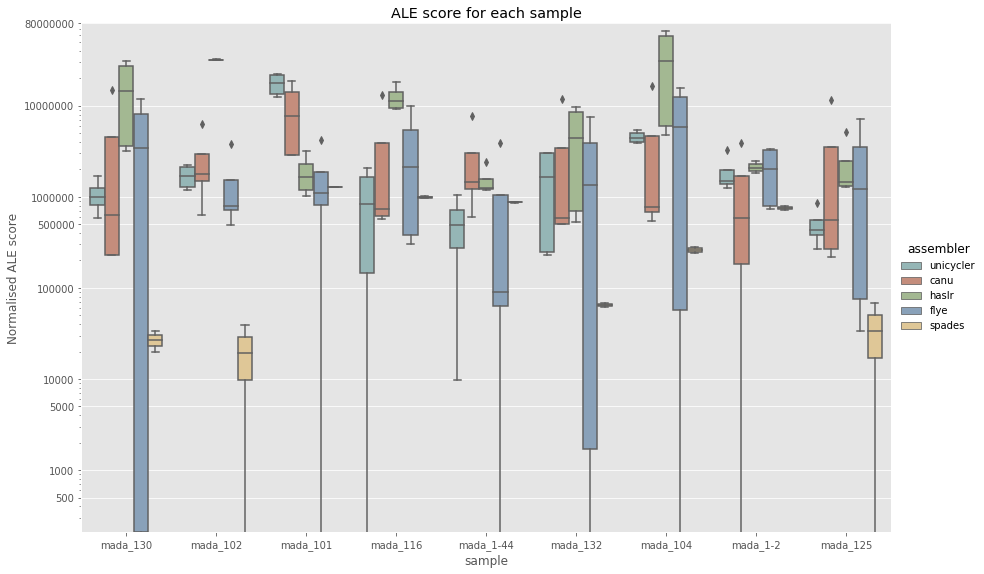
\includegraphics[width=1.0\textwidth]{Chapter2/Figs/ale_score.png}
\centering
\caption{The normalised ALE score (Y-axis) for each sample (X-axis), coloured by assembly tools. ALE score is a metric describing the likelihood of an assembly. The normalisation is done by subtracting the assembly's score from the maximum (best) score for that sample, giving a relative probability of correctness. Each box represents different technologies and polishing status for each assembler.}
\label{fig:ale_score}
\end{figure}



\subsubsection{Disagreement rate}

The disagreement rate is an approximation of the per-base accuracy of the assembly (see Methods\todo{link to relevant methods section}). In short, we map Illumina reads to the assembly and calculate what proportion of positions do XXX\% of the reads agree with the assembly nucleotide.  

In 7/9 samples, a \vrb{HASLR} assembly had the lowest disagreement rate, followed by \vrb{unicycler} having the minimum in 2/9. Polished genomes produced the lowest disagreement rate in 8/9 samples and \ont{}-based assemblies had the best accuracy in 6/9 samples. While it isn't so surprising that assemblies polished with Illumina reads have a lower disagreement rate, it is unexpected that \ont{} would produce more accurate assemblies (\autoref{fig:disagree_rate}). One caveat to keep in mind here - and this is the reason for looking at many different metrics - is that there is an element of overfitting to this metric: we assess using Illumina, and so naturally, assemblies polished with Illumina produce better results. That is not to say this statistic is void, but that it should be used with caution.



\begin{figure}
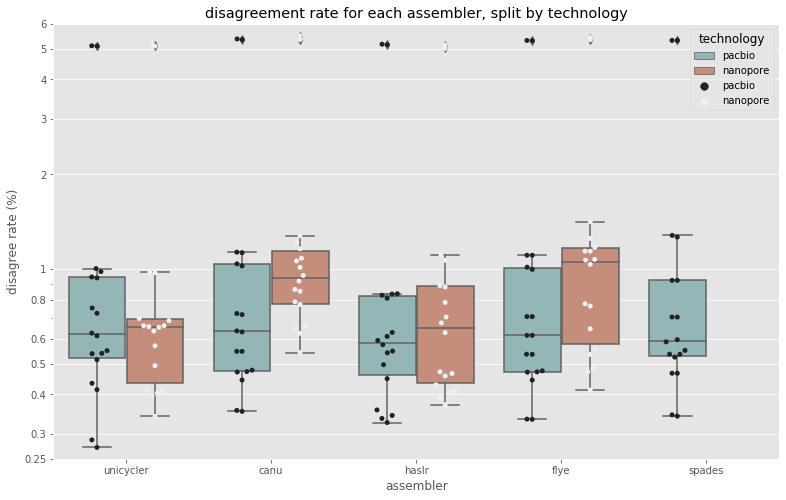
\includegraphics[width=1.0\textwidth]{Chapter2/Figs/disagree_rate.png}
\centering
\caption{The disagreement rate (Y-axis) for each assembler (X-axis), coloured by the sequencing technology. Disagreement rate is the percentage of sites in the assembly where Illumina reads do not have XX\% quorum. Each box/point represents different samples and polished status for the relevant assembler-technology combination.}
\label{fig:disagree_rate}
\end{figure}



\subsubsection{Number of contigs}

As \mtb{} has only a single, circular chromosome, for an assembly to be structurally complete, there should only be a single contig in the final assembly. However, it is not always appropriate for an assembly method to produce a single contig as data quality, depth of sequencing, read length, and/or repetitive content of the genome can hamper this goal(CITE). Conversely, receiving a single contig as output is no guarantee of it's quality for similar reasons to the previous, multi-contig scenario. For the purposes of this benchmark, considering on conjunction with the other metrics, the number of contigs can be a useful datum for selecting our favoured assembly. If an assembly has a single contig, and scores well on other metrics, we would be more inclined to choose it over another assembly with similar metrics, but many more contigs.

Across all combinations of assembly conditions, \vrb{spades} (8/18), \vrb{flye} (18/32) and \vrb{canu} (16/32) produced far more single-contig assemblies than the hybrid methods (\autoref{fig:num_contigs}). \vrb{unicycler} produced no single-contig genomes, whilst \vrb{HASLR} yielded only 2/32. When considering sequencing technology, CCS (26/72) had many more single-contig assemblies than \ont{} (10/72). Note: \vrb{spades} assemblies use all three technologies and are not considered in the technology single-contig totals.



\begin{figure}
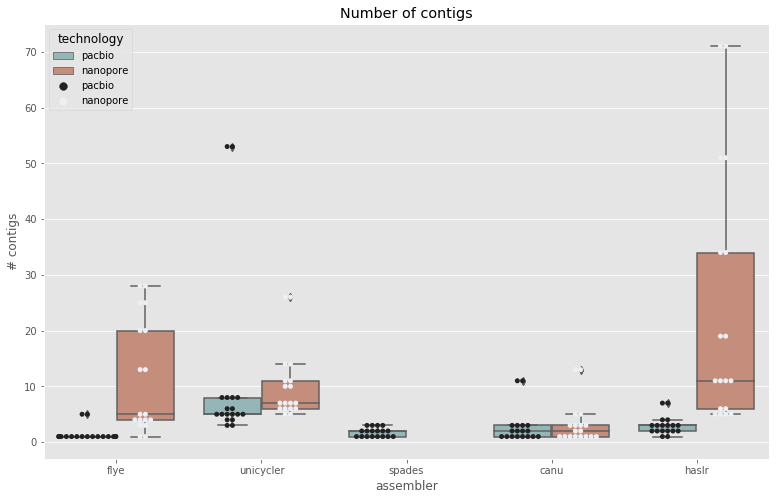
\includegraphics[width=1.0\textwidth]{Chapter2/Figs/num_contigs.png}
\centering
\caption{The number of contigs (Y-axis) produced from each assembly (X-axis), coloured by sequencing technology. Each box/point represents different samples and polished status for the relevant assembler-technology combination.}
\label{fig:num_contigs}
\end{figure}



\subsubsection{Length of assembly}

As mentioned earlier, comparing the assemblies to the \mtb{} reference genome (H37Rv; accession: `NC\_000962.3`) is not appropriate, however, it's length/size can be used as an aid for selection. The size of the any lineage's genome is not expected to differ from the reference by more than about X kilobases(CITE). Considering the genome size in addition to disagreement rate is particularly informative. It would be quite easy for an assembly method to produce very accurate per-base contigs but refusing to produce sequence for "harder" parts of the genome. While such an assembly would score well on disagreement rate, it would not do so well when considering how close to the expected genome size it is. The length of the assembly is also clearly shows when a method is outputting \textit{too much} sequence.

When comparing the size of each assembly to that of H37Rv, we found a fairly even spread across assemblers for the closest size to H37Rv. For 3/9 samples, \vrb{canu} has the smallest size difference, followed by \vrb{spades} (2/9), \vrb{unicycler} (2/9), \vrb{HASLR} (1/9) and \vrb{flye} (1/9). An honourable mention should be made of \vrb{flye} and \vrb{spades} as they had much lower variation in size compared to the other approaches. In terms of sequencing technology, in 6/9 samples CCS produced the genome size closest to H37Rv. Polished assemblies had the closer size in 5/9 samples.



\unsure[inline]{should I use the non-zoomed version of \autoref{fig:asm_len}?}
\begin{figure}
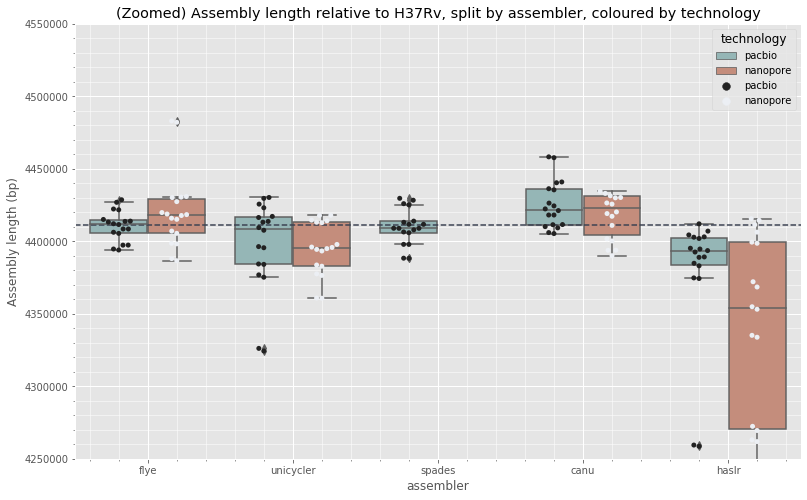
\includegraphics[width=1.0\textwidth]{Chapter2/Figs/asm_len.png}
\centering
\caption{Size/length (Y-axis) of each assembly (X-axis), coloured by each sequencing technology. The horizontal dashed line represents the size of the \mtb{} reference genome (4,411,532bp). Each box/point represents different samples and polished status for the relevant assembler-technology combination. Note: the Y-axis has been limited to allow for greater resolution of similarity to the H37Rv size}
\label{fig:asm_len}
\end{figure}



\subsubsection{Contamination detection}

The decontamination step in the assembly pipeline (\todo{reference relevant section in methods}) revealed that one sample, `mada\_1-2`, contained contigs from three different species: *Mycobacterium intracellulare*, *Dermacoccus nishinomiyaensis*, and *M. tuberculosis*. These contigs were all at sufficient coverage to not be considered background noise. For the assembly assessment analysis only the contigs from \mtb{} were used, but figures for the assessment metrics in the previous subsections show this sample is an outlier in almost all metrics. Given this profuse contamination, `mada\_1-2` will not be used in any analysis where these assemblies are used for truth validation purposes.


\unsure{should this paragraph stay here or move to the conclusion?}In conclusion, considering all assessment metrics, \vrb{flye} and \vrb{spades} assemblies were consistently the better performing methods across all of the criteria outlined in this section. As most of the validation analyses that these assemblies will be used for involve comparing Illumina and \ont{} data to a "neutral truth", the unpolished CCS assemblies from \vrb{flye} were selected for use in the remainder of this chapter. The differences between the polished and unpolished CCS assemblies was almost negligible and do not outweigh the benefit of having a single-technology PacBio assembly that can be used as an unbiased reference point for comparing the other two technologies.

%=========================================================================

\section{Quality control of samples}
\label{sec:ch2-qc}

Prior to any variant calling, all samples were subjected to a quality control (QC) pipeline to ensure all data used was of the highest quality. The QC pipeline was written in \vrb{snakemake}(CITE) and an overview of the steps can be seen in (FIGURE). \\
The first step in QC is decontamination of both Illumina and \ont{} sequencing reads. We use the decontamination database from \vrb{clockwork}(CITE), which contains a wide range of organisms, including viral, human, \mtb{}, NTM, and nasopharyngeal-associated bacterial genomes. Each genome has associated metadata indicating if it is contamination or not. Reads are mapped to the database using `bwa mem`(CITE) (Illumina) and \vrb{minimap2}(CITE). The resulting alignment is used to quantify the proportion of reads considered contamination, unmapped, and wanted. A read is considered wanted if it has any mapping to a non-contamination genome in the database and is output to a final decontaminated fastq file. All other mapped reads are considered contamination. Interactive \vrb{krona}(CITE) charts (see FIGURE\change{move the reference to the krona chart to the results section}) are used to visualise a sample's composition based on the decontamination database alignment.  

All decontaminated fastq files were subsampled to a depth of 60x (Illumina) and 150x (\ont{}) using \vrb{rasusa}(CITE). The reason for subsampling is to limit unnecessarily large read sets that can drastically slow down later steps in the analysis process and do not provide any benefit\unsure{see if there is a reference that backs this up}. Any sample with depth less than the maximum threshold remains unchanged.  

The last step in the QC pipeline is to assign lineages for each sample. A panel of lineage-defining SNPs from (CITE) is used in conjunction with a sample's VCF from the Illumina variant calls(LINK) for the lineage assignment. At each lineage-defining position in the sample's VCF we determine if the called allele is the same as the panel allele. If it is, we add the full lineage that allele defines (e.g. 4.1.1) to a list of called lineages. For this analysis, if more than one heterozygous call was made at lineage-defining positions, we abandon lineage assignment for that sample. After classifying all of a sample's lineage-defining positions we then produce a lineage assignment based on the list of called lineages. The most recent common ancestor of all the called lineages is used as the lineage assignment. For example, if the called lineages were [4, 4.2.3, 4.2.5] the lineage assignment would be 4.2. If there is more than one called lineage from a different major lineage group, a mixed lineage assignment is given. For example [4, 4.2.3, 4.2.5, 3.2] would still be called lineage 4.2, however, [4, 4.2.3, 4.2.5, 3.2, 3.1] would be called mixed.

The purpose of QC is to ensure all samples used in later analysis are of the highest quality. By highest quality we mean all samples have perfectly matched Illumina and \ont{} data, sufficient coverage on both sequencing technologies, no contamination, and no evidence of a mixed \mtb{} population. Prior to the QC stage, N samples were excluded as their Illumina and \ont{} reads were not from the exact same DNA extraction.  

After filtering out unmapped/contaminant reads and subsampling all samples to 60x (Illumina) and 150x (\ont{}), N samples were excluded from further analysis due to low coverage (FIGURE) - defined as Nx for Illumina and Nx for \ont{}. An example chart of the composition of genomes from the decontamination database for a sample can be seen in (FIGURE).  

Lastly, N samples were excluded as their lineage assignment was either called mixed or unknown. Unknown lineage assignments can happen if the sample has too many heterozygous calls as lineage-defining positions, or there was no called lineages at any lineage-defining position.  

In the end, we have N samples that have passed QC and will be used for the remainder of this chapter.

\towrite[inline]{Make sure to mention the samples excluded as their Illumina and ONT data do not match based on the discrepancy in variant calls}


%=========================================================================

\section{Construction of \mtb{} reference graphs}
\label{sec:tbprg}

% https://github.com/mbhall88/head_to_head_pipeline/issues/10 and https://github.com/mbhall88/head_to_head_pipeline/issues/9 have some good plots/stats to include here
\pandora{} requires a \prg{} in order to operate. For the work in this chapter, we chose to construct a reference \prg{} based on the \mtb{} reference genome, H37Rv. We add variants sampled from 15000 global \mtb{} isolates gathered by the \cryptic{} consortium\improvement{confirm this number and see if there is a reference for the samples}. We sampled at two different rates to evaluate how varying complexity of \prg{}s affect variant-calling precision and recall.

To ensure the reference \prg{} is not biased towards a particular lineage we first split the global \cryptic{} VCF into separate lineage VCFs. Lineages were determined for each of the global samples using the same approach as in \autoref{sec:ch2-qc}. Lineages 1-4 were separated into separate VCF files and all other lineages were grouped into a single VCF due to much smaller representation. Variants calls from 14 high-quality \mtb{} assemblies, representing lineages 1-7, were also included in this "other" lineage VCF. The two \prg{} complexities we chose to construct were termed "sparse" and "dense". From each lineage VCF, we took a random subsample of 50 and 200 samples and combined them into single sparse and dense VCFs respectively. It should be noted that we use the same fixed random seed for the subsampling to ensure the sparse \prg{} is a subset - with respect to the sample variants - of the dense \prg{}. We filtered the resulting VCFs to remove any positions with no alternate allele calls, or that failed the filtering applied by the \cryptic{} pipeline (except for masked positions).  

The \prg{} that \pandora{} uses as it's reference is actually a collection of local \prg{}s (loci). These loci are effectively partitions of the original genome; one can partition based on any criteria they like. For the work in the chapter, we chose to split the H37Rv genome based on the genomic features outlined in the accompanying General Feature Format (GFF). We also retain the segments *between* the features - so called intergenic regions (IGRs). We combine genomic features that have overlapping coordinates (i.e. they are transcribed on opposite strands or different reading frames) into a single locus and also join any locus (feature or IGR) shorter than 500bp with its 3' neighbour. By building the reference \prg{} in this manner we ensure that every position in the H37Rv genome is represented in one of the local \prg{}s. We then remove any locus with 30\% or more of its positions overlapping a genome mask of repetitive regions in H37Rv \cite{tbmask2014}. Refer to \autoref{app:mask} for a detailed description of why this masking strategy was chosen.

We form the sparse and dense \prg{}s by applying the variants from their VCF to the template sequence of each locus for the corresponding genomic position. For each position in the VCF, we infer the locus it corresponds to. We then take all (called) alternate alleles and create a sequence for each; that is, the template sequence, with the reference allele starting at the position replaced with the alternate allele. Note, we disregard any indels longer than 20bp or that span a locus boundary. All of these sequences are pooled into a single fasta file for each locus. 

The multi-sequence fasta files are then subjected to multiple sequence alignment (MSA) using MAFFT(CITE). We use the accurate global alignment setting, G-INS-i(CITE\info{citation in Papers library under msa tag}), with default parameters, using the \vrb{ginsi} script provided with MAFFT. The resulting MSA is then converted to a \pandora{}-compatible \prg{} using the `make\_prg` script(CITE) with a maximum nesting level of 5 and maximum match length of 7. All of the local \prg{}s are then combined into a single \prg{} file and indexed with \pandora{} using a \kmer{} size of 15 and window size of 14. In the end, we have two single \prg{} files - sparse and dense.

\subsection{Computational performance}

An important consideration for usability of any genomic method is the computational costs such as time and resources. The construction process just outlined need only be run once and then it can be used as a reference for subsequent \pandora{} usage. However, it is important to understand the time and resources required in order to identify bottlenecks. Additionally, if the resource usage is high enough, it may also limit who is able to build their own reference graph. We outline the time and memory requirements for each step of the graph construction in \autoref{tab:build-prg}. All times are on a single compute node with 32 CPU cores. We only report the MSA, \makeprg{}, and \pandora{} index steps as these are constants that must be done this way and the steps prior to this are not very time or resource intensive and could be done in a number of different ways.

\begin{table}
\centering
\begin{tabularx}{\textwidth}{|l|l|l|l|l|l|l|}
\hline
         & \multicolumn{3}{l|}{Sparse}                          & \multicolumn{3}{l|}{Dense}                           \\ \hline
Step     & CPU time (sec) & Real time (H:m) & Max. RAM (GB) & CPU time (sec) & Real time (H:m) & Max. RAM (GB) \\ \hline%\cline{1-2} \cline{4-5} \cline{7-7} 
MSA      & 138576         & 1:16             & 209              & 445284         & 3:56             & 301              \\ \hline%\cline{1-2} \cline{4-5} \cline{7-7} 
Make PRG & 3746           & 0:04             & 0.9              & 4269           & 0:05             & 0.9              \\ \hline%\cline{1-2} \cline{4-5} \cline{7-7} 
Index    & 142            & 0:01             & 1.5              & 361            & 0:01             & 1.7              \\ \hline%\cline{1-2} \cline{4-5} \cline{7-7} 
\end{tabularx}
\caption{Computational time and memory usage for the main steps of building a \mtb{} reference graph. Sparse and Dense refer to two different densities with respect to the number of variants used. All steps were run on a single compute node with 32 CPU cores. MSA=multiple sequence alignment;PRG=population reference graph.}
\label{tab:build-prg}
\end{table}

%=========================================================================

\section{Variant-calling and calibration of \ont{} variant filters}
\label{sec:var-calls}

Filtering of variant calls is integral to creating trusted transmission
inference. There are many such filters used for Illumina genomic data
and they can produce inconsistent results\cite{walter2020}. Before
attempting to define SNP thresholds for Nanopore data, we explore the
performance of a range of filtering parameters for both bcftools and \pandora{}.  
The aim of this filter calibration is ultimately to determine if SNP-calling precision for \ont{} is comparable with Illumina, and if not, how close can we get it.
We evaluate the resulting, filtered SNP calls
against the COMPASS\todo{http://dx.doi.org/10.2807/1560-7917.es.2019.24.50.1900130} Illumina SNP calls for the seven
samples with high-quality PacBio assemblies (see \autoref{sec:asm_results}) to ensure no bias for
Illumina or Nanopore.
For others interested in investigating variant filters for \ont{} data, we also hope this calibration acts as a good starting point for deeper analysis.

\subsection{Validating variant calls}

We evaluate the precision and recall of the SNP calls using the method outlined in \todo{link to varifier stuff in chapter 1} - \vrb{varifier} - with a flank length of 100bp. The samples we evaluated are those seven with PacBio assemblies (see Section \autoref{sec:asm_results}). As a truth genome for each, we use the unpolished \vrb{flye} PacBio assembly, along with a mask for low-quality regions. These low-quality regions were identified by aligning the sample's Illumina reads to the assembly with \vrb{bwa mem} and flagging any position with less than 10 reads mapping to it or less than 90\% agreement. From the varifier output, we use the edit distance measure for both precision and recall. All results were visualised in Python using the matplotlib (version 3.1.3) (Hunter 2007) and seaborn (version 0.11.1) (Waskom 2020) libraries.

\subsection{Illumina variant calling}

Illumina variant calls were made using the COMPASS pipeline (Jajou 2019) used by Public Health England (PHE). Briefly, reads are mapped to the \mtb{} reference genome, and \vrb{samtools mpileup} is used to identify SNPs (Li 2009). SNPs are filtered based on the following criteria: i) must have at least five high-quality supporting reads, ii) must have at least one read in each direction, iii) 75\% of reads must be high-quality, iv) the diploid genotype must be homozygous, v) fraction of reads supporting the major allele must be at least 90\%. In addition, any SNPs falling within masked sites - as defined by aligning the \mtb{} reference to itself and identifying repetitive regions - are excluded.

\subsection{\ont{} variant calling: \vrb{bcftools}}
\label{sec:bcftools-filters}

As there is no standard variant caller used for \mtb{} \ont{} data, we chose to try bcftools, as it has a long history of use in bioinformatics, is one of the main variant callers used for Illumina data  and is readily available to all users, and is much more user-friendly than other available tools. Another main reason for its use is that it is the updated form of the samtools pipeline used by COMPASS. The parameters used are
relevant to the variant calls produced by the multiallelic
model\todo{http://dx.doi.org/10.1099/mgen.0.000418}.

Nanopore reads were aligned to the \mtb{} reference genome using minimap2 (version 2.17), with options to produce SAM output containing no secondary alignments. The subsequent SAM file is provided as input to the bcftools (version 1.11) subcommand \vrb{mpileup} with the 'skip indels' option. The resulting pileup is then used to call SNPs with \vrb{bcftools call} using the multiallelic caller with a haploid model and an option to skip indel variants.
There are a number of fields in the resulting VCF relating to the information about the reads that support each position. We filter VCF positions based on whether certain fields meet a given criteria.
After a thorough examination of the how filtering based on each field impacts precision and recall, we settled on five filters for bcftools. First, we filter out positions with a quality (QUAL field) score of less than 60. The quality is a log-scaled probability for the assertion made by the alternate allele. Second, read position bias (RPB) of at least 0.05 is required. RPB indicates whether there is a bias for support from the ends of reads, as they are usually low quality. Third, we filter out positions with a segregation-based metric (SGB) less than -0.5. SGB is a measure of how read depths across alleles match expected depths. Fourth, variant distance bias (VDB) less than 0.002 is filtered out. VDB is a measure of whether a variant's position within the reads that support it is randomly distributed or biased (e.g. near the start). Fifth, the fraction of reads supporting the called allele (FRS) must be 90\% or more.

\autoref{fig:bcftools-filters} shows the precision (proportion
of calls that are correct) and recall (proportion of variants found) for
a selection of these bcftools VCF fields. The trade-off between
precision and recall is dependent on the question one is trying to
answer. For the purposes of transmission clustering, we place higher importance on
precision as we seek to ensure the calls used are of the highest
quality. The consequence of this is we miss some variants - compared to
COMPASS.

The filtering we use for the remainder of the transmission inference
work is to remove any VCF record (variant) with a quality score (QUAL)
of less than 60,~ a read position bias (RPB) of less than 0.05, variant
distance bias (VDB) less than 0.002, a fraction of read-support (FRS)
less than 0.9, and a segregation-based metric (SGB)~ greater than -0.5.
These filters, represented by the yellow box in
Figure~{\ref{fig:bcftools-filters}}, lead to median precision and
recall of 99.94\% and 84.26\%, respectively for the seven validation
samples. When compared to the COMPASS median precision and recall values
of 100\% and 92.58\%, respectively,~ we produce Nanopore variant calls
with equivalent precision to Illumina, but with less recall.

\begin{figure}
\begin{center}
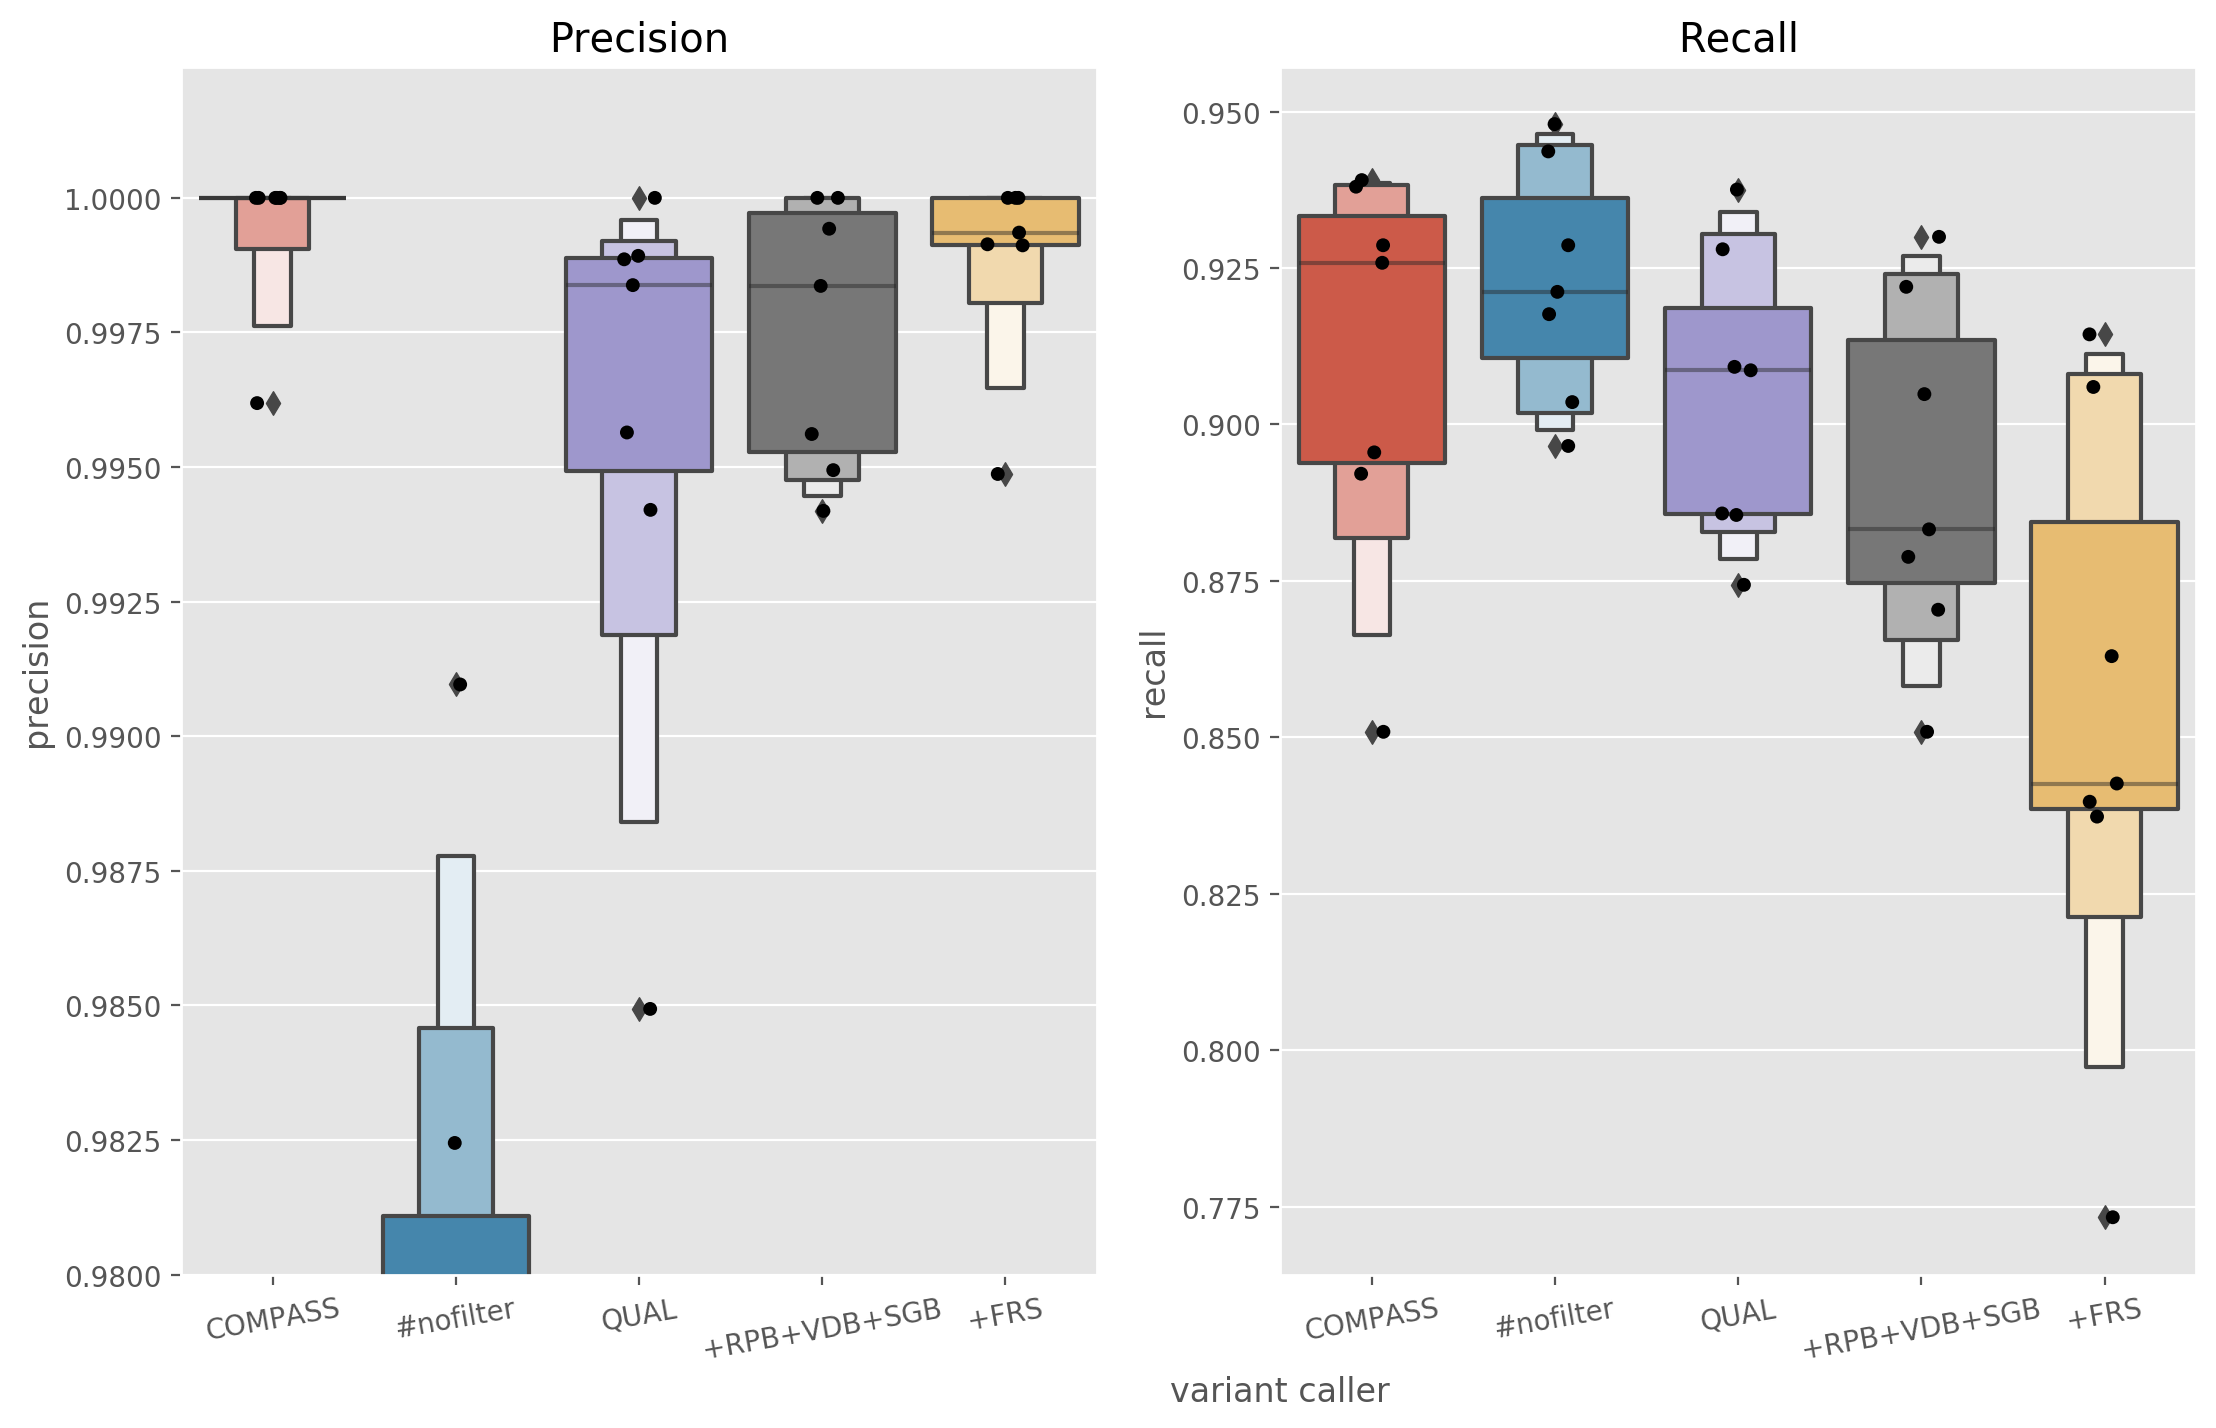
\includegraphics[width=0.90\columnwidth]{Chapter2/Figs/bcftools-precision-recall-filters.png}
\caption{{Precision (left) and recall (right) of SNPs for COMPASS (red) and a
selection of bcftools filters. `\#nofilter' (blue) is bcftools with no
filtering of variants. `QUAL' (purple) is bcftools SNPs with a quality score of
60 or more. `+RPB+VDB+SGB' (grey) indicates bcftools variants with the INFO
field values~\(\ge\)0.05,~\(\ge\)0.002,
and~\(\le\)-0.5, respectively, plus QUAL. `+FRS' (yellow) shows
bcftools SNPs with all previous filters, plus only SNPs where the
fraction of reads supporting the variant is at least 90\%. Note: the
precision plot y-axis was cut causing some `\#nofilter' points to be
hidden.
{\label{fig:bcftools-filters}}%
}}
\end{center}
\end{figure}

\subsection{\ont{} variant calling: \pandora{}}
\label{sec:pandora-filters}

When assessing the best filters for increasing the precision of variant calls from \pandora{}, we are also interested in determining whether \prg{} density has a noticeable impact on performance. We use the sparse and dense \prg{}s from \autoref{sec:tbprg} and look at precision and recall these produce for the same filters.

\subsubsection{Single-sample}
\label{sec:map-var-calls}

For each sample, we discover \denovo{} variants using the method outlined in \autoref{chap:denovo} using the \vrb{discover} command of \pandora{} (version 0.8.0), using default parameters except for limiting the number of novel variants for a candidate region to 10. Novel variants are added to the relevant \prg{} using the same method as \todo{reference chapter 1 section that outlines how we feed de novo variants back into the PRG} and the resulting, update \prg{}s are indexed with \pandora{}. The \vrb{map} routine of \pandora{} is then used to genotype the sample's reads and produce a VCF. To be able to compare the \pandora{} VCF to the truth assemblies we tell \pandora{} to output coordinates with respect to the H37Rv reference sequence for each locus. Then, we convert these locus positions to the absolute position within H37Rv. Running \pandora{} in this way leads to some alleles being quite long and having a lot of redundant information, so we use bcftools norm to trim unused alleles and reduce variants down to their most succinct representation.
The \pandora{} VCF fields we use for filtering are: the depth of coverage on the called allele, which we require at least 3 reads; we keep positions with a strand bias of at least 1\%, which is the lowest depth on the forward or reverse strand divided by the total depth; a genotype confidence score no less than 5; an FRS of at least 90\%  - calculated the same way as in \autoref{sec:bcftools-filters}.
The results of incrementally applying these filters, along with no filters and COMPASS, are shown in \autoref{fig:pandora-filters-snps}. \pandora{}'s best median precision (100\%) and
is with a sparse \prg{} and all filters applied. With all filters, the sparse \prg{} leads to a median recall of 71.99\%. When compared to the COMPASS median precision and recall values
of 100\% and 92.58\%, respectively, \pandora{} produces Nanopore variant calls
with equivalent precision to Illumina, but with 20.59\% less recall. Part of the recall disparity between \pandora{} and COMPASS is explained by the masking of loci in the reference graph (see \autoref{sec:tbprg} and \autoref{app:mask}). Despite this large difference in recall, we chose to use all of the filters outlined above because, as mentioned earlier, precision is far more important than recall for the transmission cluster work.
In nearly every filtering combination, the sparse \prg{} lead to higher recall \emph{and} precision, albeit quite marginal. As a result, the remaining work featuring \pandora{} in this chapter will use the sparse \prg{}. Given the increased computational cost of using the dense \prg{}, without any benefit for precision and recall.

\begin{figure}
\begin{center}
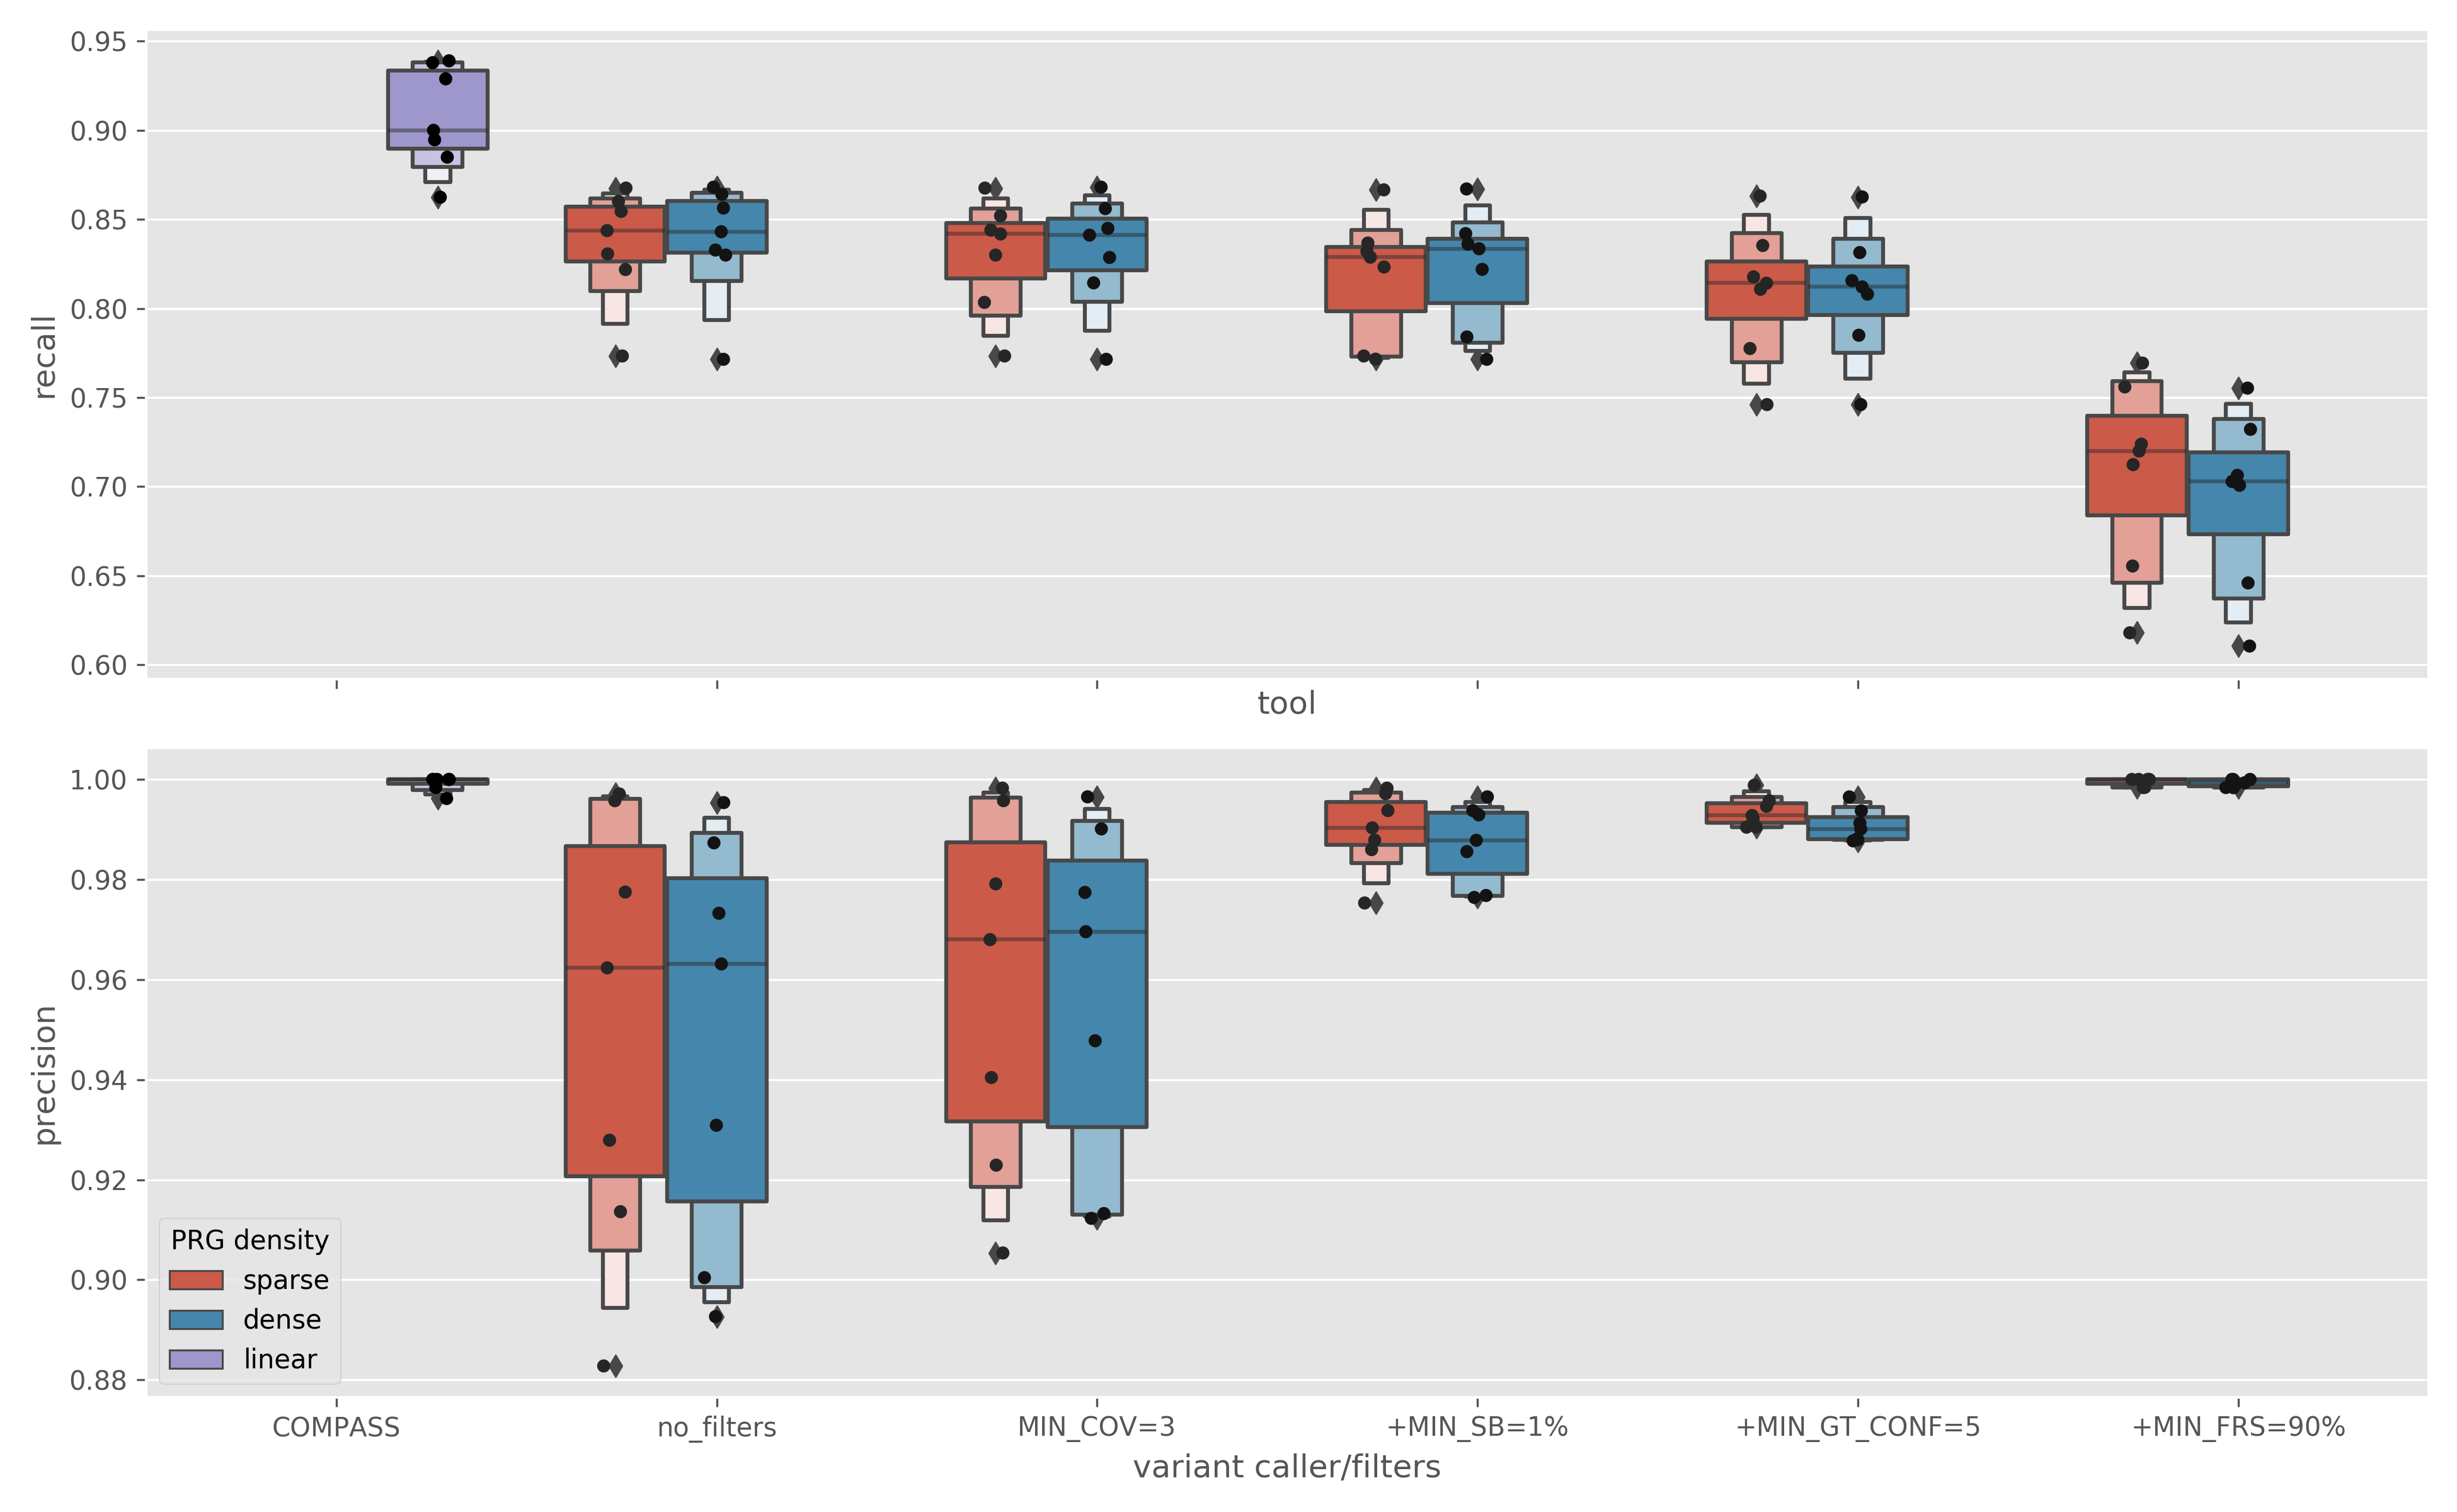
\includegraphics[width=0.90\columnwidth]{Chapter2/Figs/pandora-precision-recall-filters-snps.png}
\caption{{Precision (bottom) and recall (top) of SNPs for COMPASS (purple) and \pandora{} with sparse (red) and dense (blue) \prg{}s. The \pandora{} boxes start with no filters on the left, with each box moving to the right adding a filter to the previous box. The COMPASS box is a reference to the precision and recall of Illumina variant calls. Linear PRG density refers to the fact that COMPASS uses a single, linear reference genome as opposed to \pandora{}, which uses a genome graph. The black points refer to single data points for the seven samples used. MIN\_COV=minimum depth of coverage;MIN\_SB=minimum strand bias;MIN\_GT\_CONF=minimum genotype confidence score;MIN\_FRS=minimum fraction of read support.
{\label{fig:pandora-filters-snps}}%
}}
\end{center}
\end{figure}

Although we only use SNPs for identifying transmission clusters, we also assessed \pandora{} variant calls for all variants, including indels up to a length of 20bp in \autoref{fig:pandora-filters-all}.  We did this for the sake of future work that might be interested in using \pandora{} indel calls, such as predicting drug resistance. Again, the sparse \prg{} gave better precision and recall than the dense one. Using all variants, there was a recall improvement to 75.48\% (all filters) - up 3.49\% from SNPs only. Precision on the other hand sees a drop to 95.90\% when assessing all variants - compared to 100\% for SNPs only. Given the large drop in precision it is clear that \pandora{} indel-calling needs further improvement, however, indel calling (deletions especially) are a known limitation of \ont{} \cite{jain2018,wick2019}.

\begin{figure}
\begin{center}
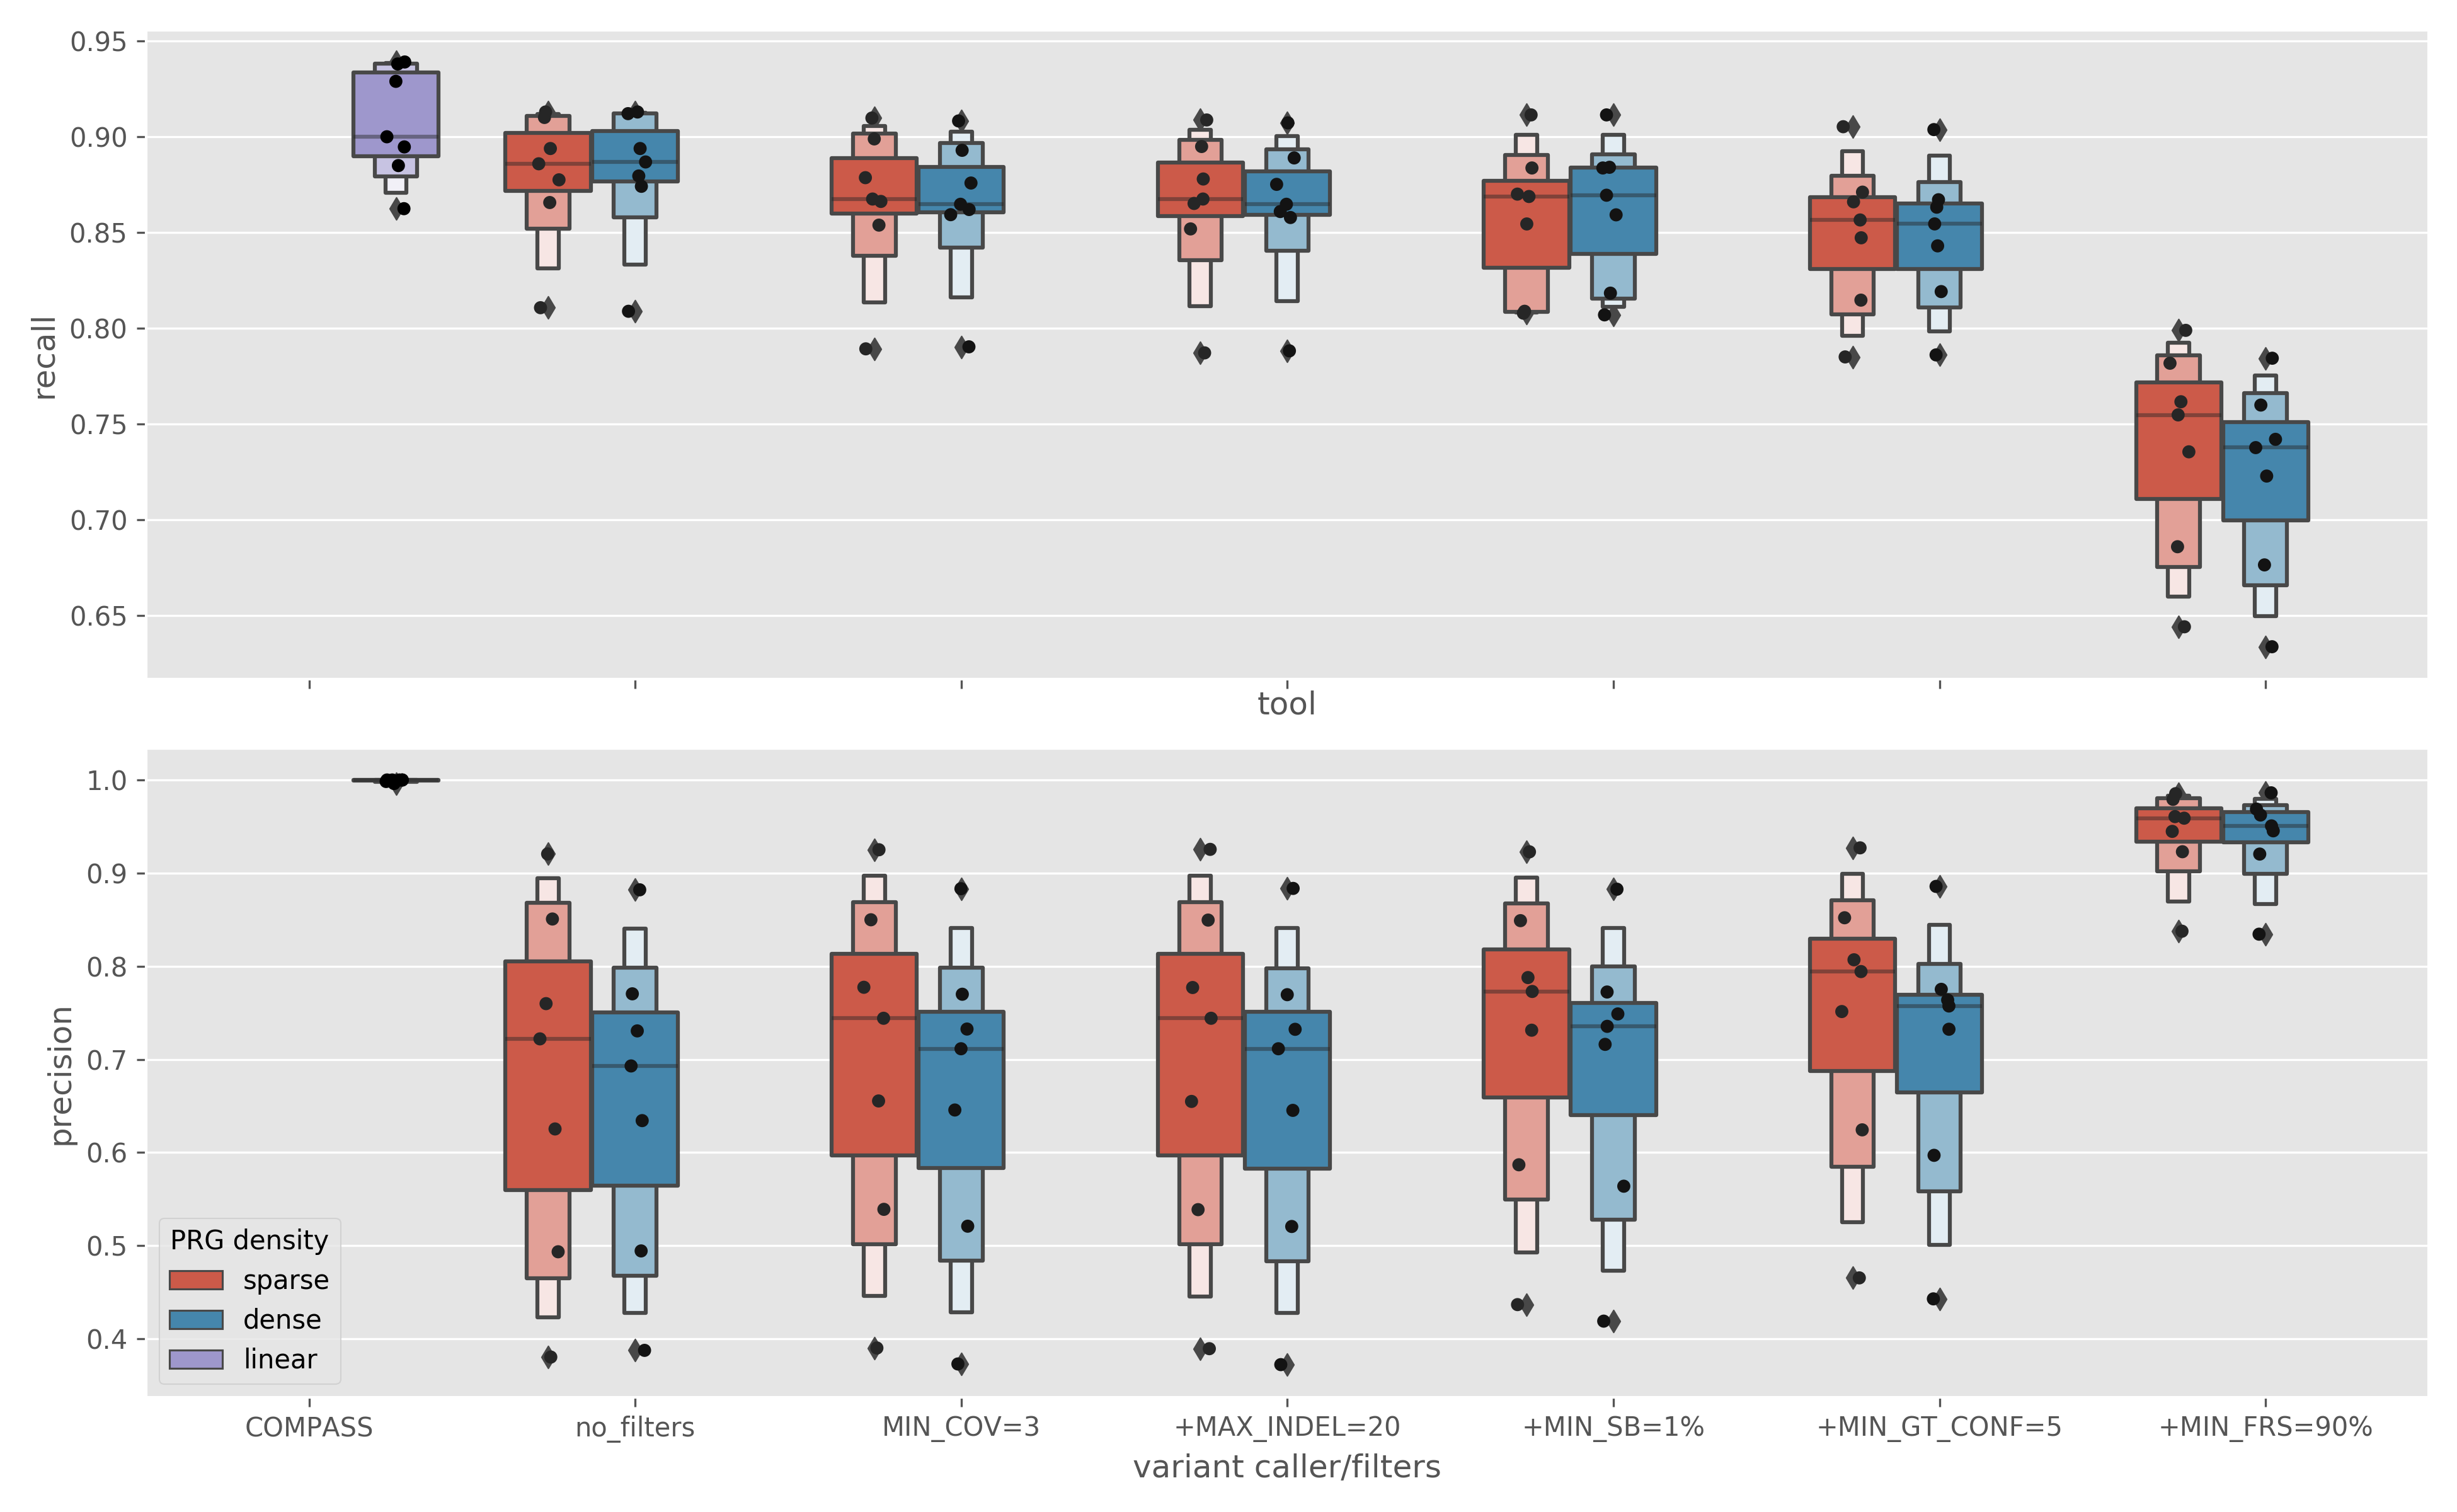
\includegraphics[width=0.90\columnwidth]{Chapter2/Figs/pandora-precision-recall-filters-all-variants.png}
\caption{{Precision (bottom) and recall (top) of SNPs for COMPASS (purple) and all variants (maximum indel length of 20bp) for \pandora{} with sparse (red) and dense (blue) \prg{}s. The \pandora{} boxes start with no filters on the left, with each box moving to the right adding a filter to the previous box. The COMPASS box is a reference to the precision and recall of Illumina variant calls. Linear PRG density refers to the fact that COMPASS uses a single, linear reference genome as opposed to \pandora{}, which uses a genome graph. The black points refer to single data points for the seven samples used. MIN\_COV=minimum depth of coverage;MIN\_SB=minimum strand bias;MIN\_GT\_CONF=minimum genotype confidence score;MIN\_FRS=minimum fraction of read support.
{\label{fig:pandora-filters-all}}%
}}
\end{center}
\end{figure}

\subsubsection{Multi-sample}

\pandora{}'s \vrb{map} routine infers a consensus sequence for a single sample and outputs variant calls with respect to that. However, \pandora{} also has a multi-sample counterpart - \vrb{compare}. The \vrb{compare} routine infers a consensus sequence for \emph{all} samples and outputs a locus presense-absence matrix, along with a VCF with genotypes for all samples with respect to the consensus sequence \todo{link to ch1 or 2 section describing compare}. As it was designed for analysing collection of (potentially divergent) samples, we use the \vrb{compare} protocol to assess its ability to describe transmission clusters. 

The process for calling variants using compare is to first take the novel variants discovered for each sample in \autoref{sec:map-var-calls}. Instead of creating an updated \prg{} for each sample, we take all novel variants for all samples and add them to the relevant locus' original MSA. We then update the MSA, rebuild the \prg{}s for each locus, combine all \prg{}s into a single PanRG and then index with \pandora{}. In the end, we have a \prg{} that has novel variants from all samples contained within it, rather than the \prg{}s used by `map` which only have the novel variants for a single sample.
Next, we run `pandora compare` using the updated sparse and dense \prg{}s and filter the resulting VCF as-per \autoref{sec:pandora-filters}.

As a result of its design, it is not possible to provide `compare` with a reference to base VCF coordinates off (as in \autoref{sec:map-var-calls}). Therefore, we cannot assess the precision and recall for the seven samples as above. We maintain the same filtering strategy as the single-sample approach though, as all of those fields are available in the VCF from `compare`.

\subsection{Computational performance}
\label{sec:var-call-comp-perf}

In addition to the quality of the variant calls, the computational cost of running them is also important. The CPU time and maximum memory usage for performing the \ont{} variant calling is shown in \autoref{fig:var-comp-perf}. \pandora{}'s performance is broken down into the individual stages, while bcftools is represented by a single job. The median maxmimum memory for bcftools was 8.2GB, although, the maximum was as high as 58.5GB. This is compared to the highest \pandora{} step - updating the MSAs with novel variants - with a median maximum memory usage of 9.7GB and 13.3GB for the sparse and dense \prg{}s respectively. The highest memory usage for \pandora{} was 18.6GB during the updating of MSAs, nearly 40GB lower than the peak of bcftools. The median CPU time for bcftools was 35129 seconds, or 9.75 hours, with the longest run coming in at 138364 seconds (38.4 hours). To be able to compare this with \pandora{} as a whole, we can sum the median CPU time over each step, which gives 21704 and 53194 seconds, or 6.0 and 14.7 hours, for the sparse and dense \prg{}s respectively. As with the memory usage, the longest runtime component of the \pandora{} pipeline was updating the MSAs with \denovo{} variants.

The computational performance of \pandora{} `compare` is not directly comparable to bcftools and \pandora{} `map` as it runs on all samples at the same time. Additionally, the novel variant discovery phase of pandora map for all samples technically contributes to the overall runtime of compare. As the performance of this discovery step has already been reported, we outline the remainder of the steps involved in compare. In total, the remainder of the sparse and dense \prg{} steps took 58.4 and 83.1 CPU hours respectively. The actual wall clock time for these steps was 5.5 and 7.3 hours. The maximum memory was again obtained during the updating of the MSAs and peaked at 38 and 37GB for the sparse and dense \prg{}s respectively.

\begin{figure}
     \centering
     \begin{subfigure}[b]{0.475\textwidth}
         \centering
         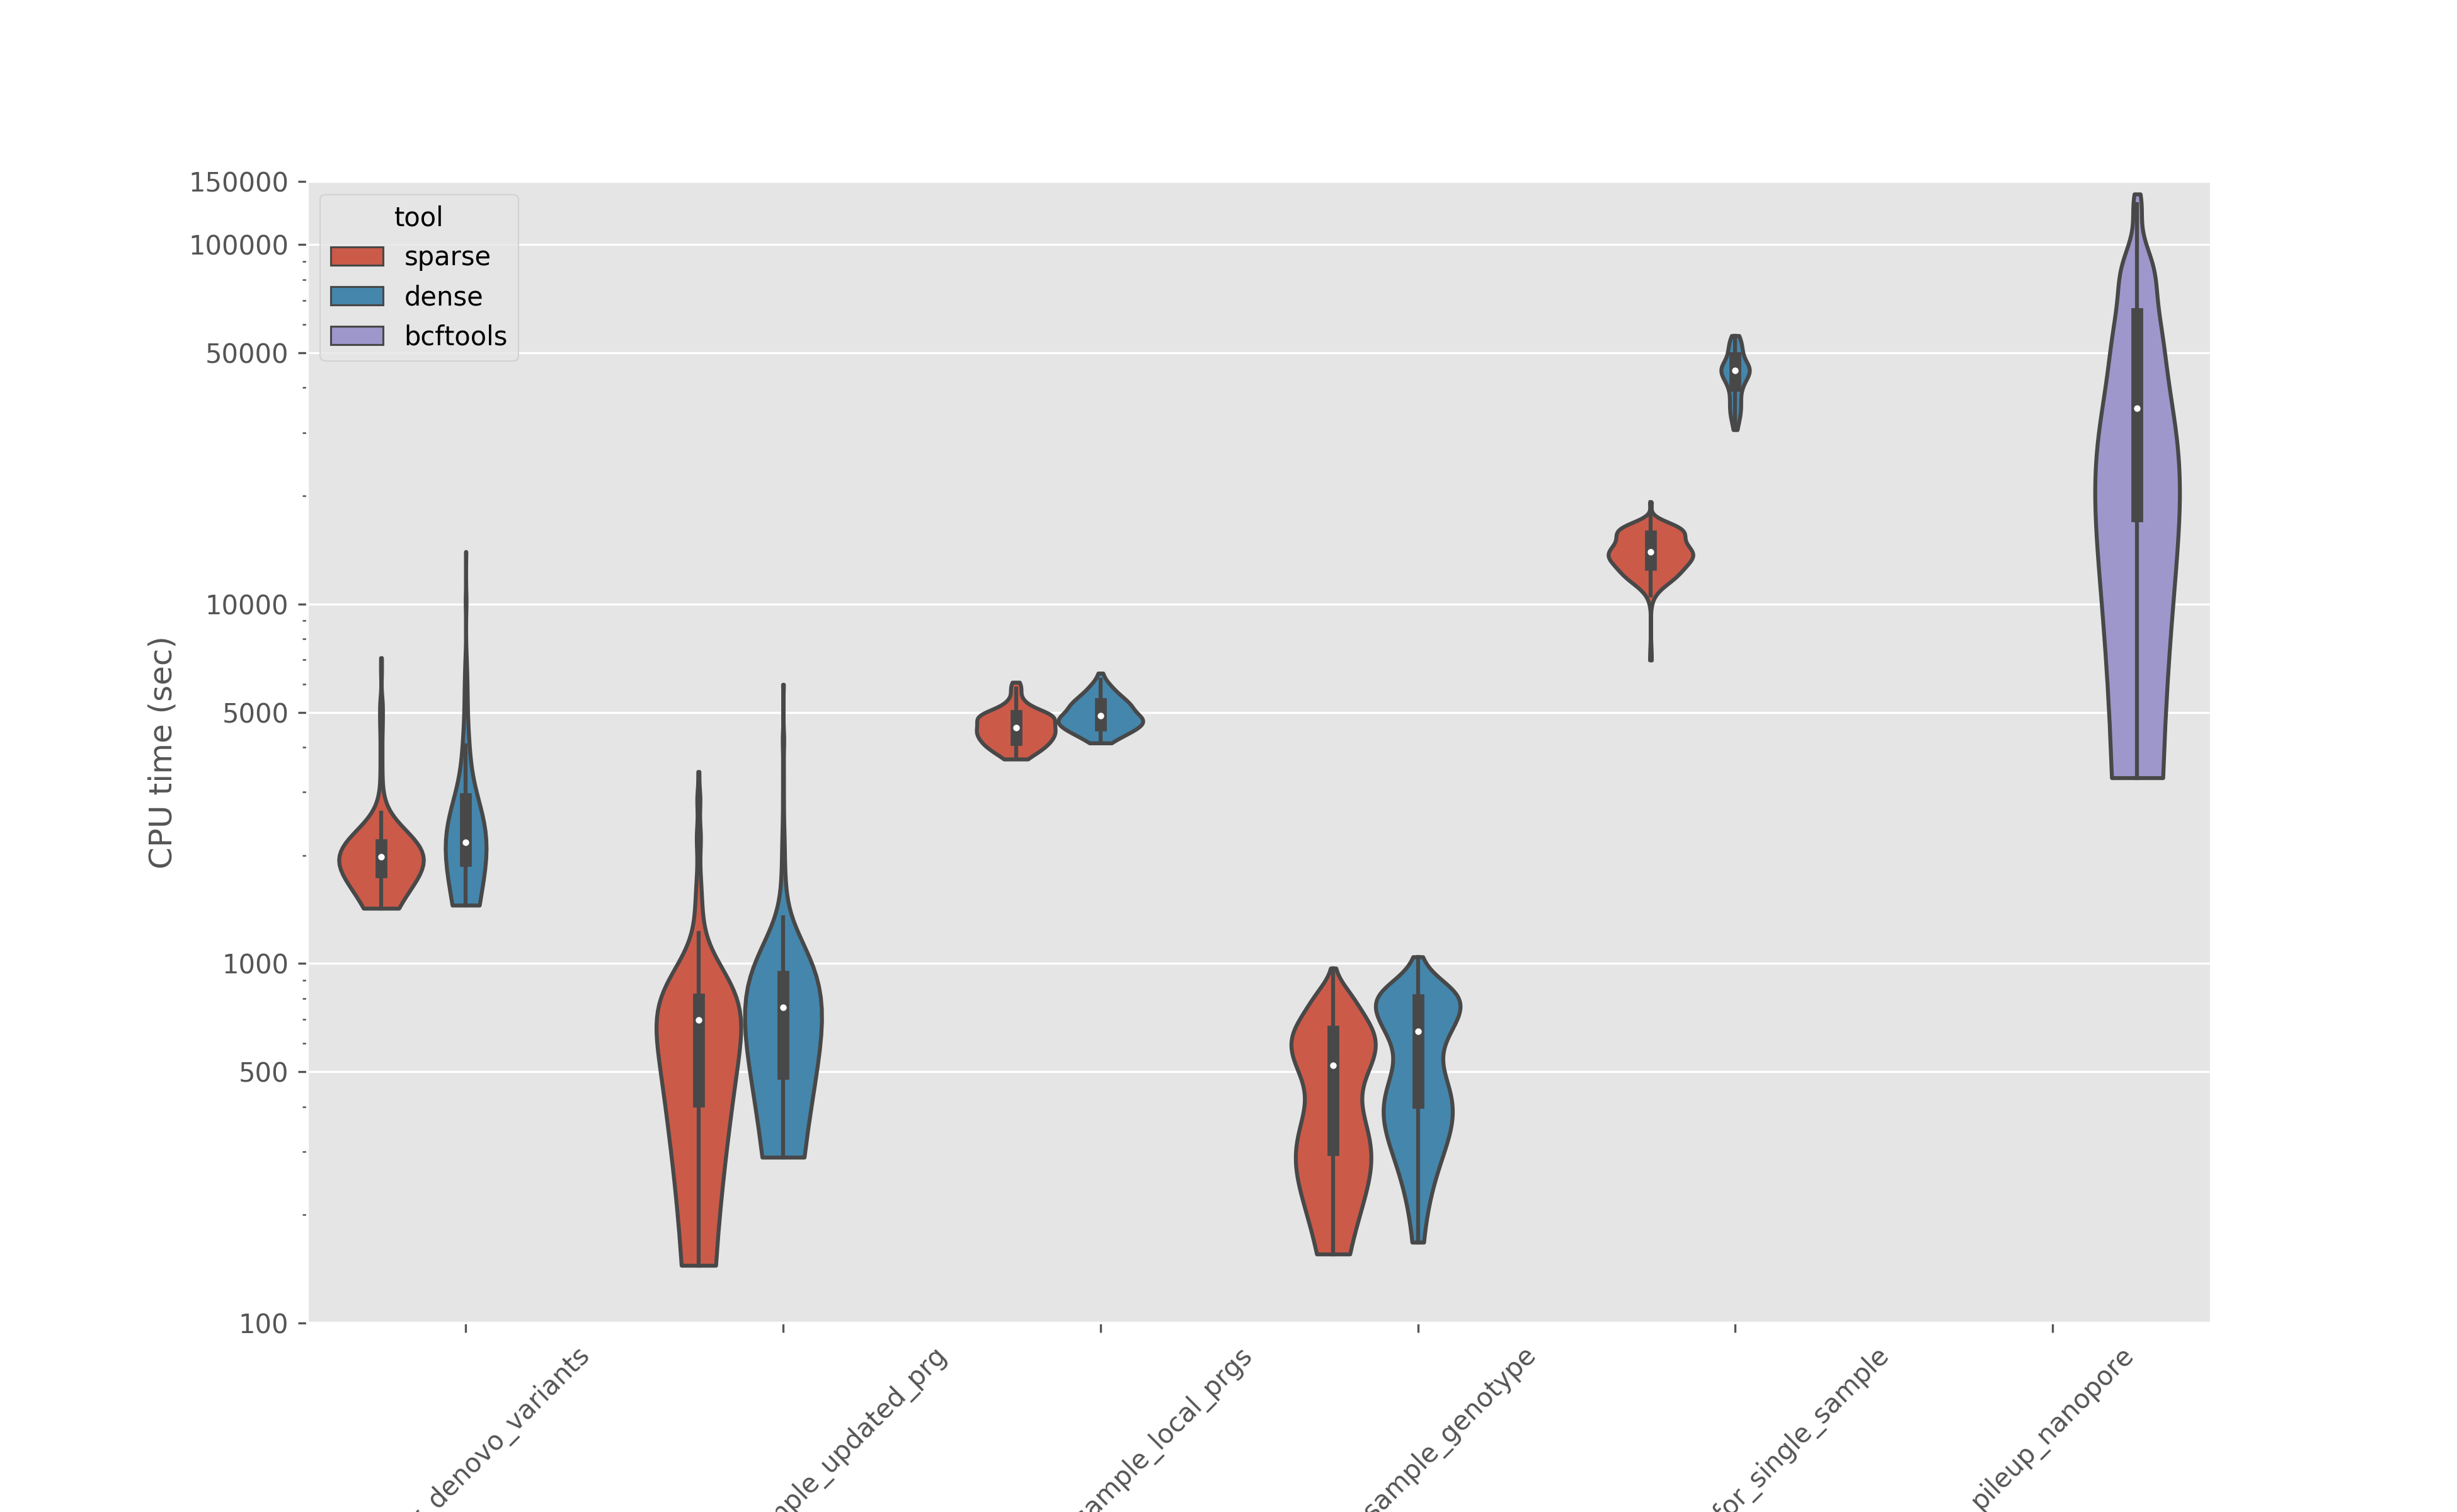
\includegraphics[width=\textwidth]{Chapter2/Figs/cpu_time.png}
         \caption{}
         \label{fig:cpu-time}
     \end{subfigure}
    %  \hfill
     \begin{subfigure}[b]{0.475\textwidth}
         \centering
         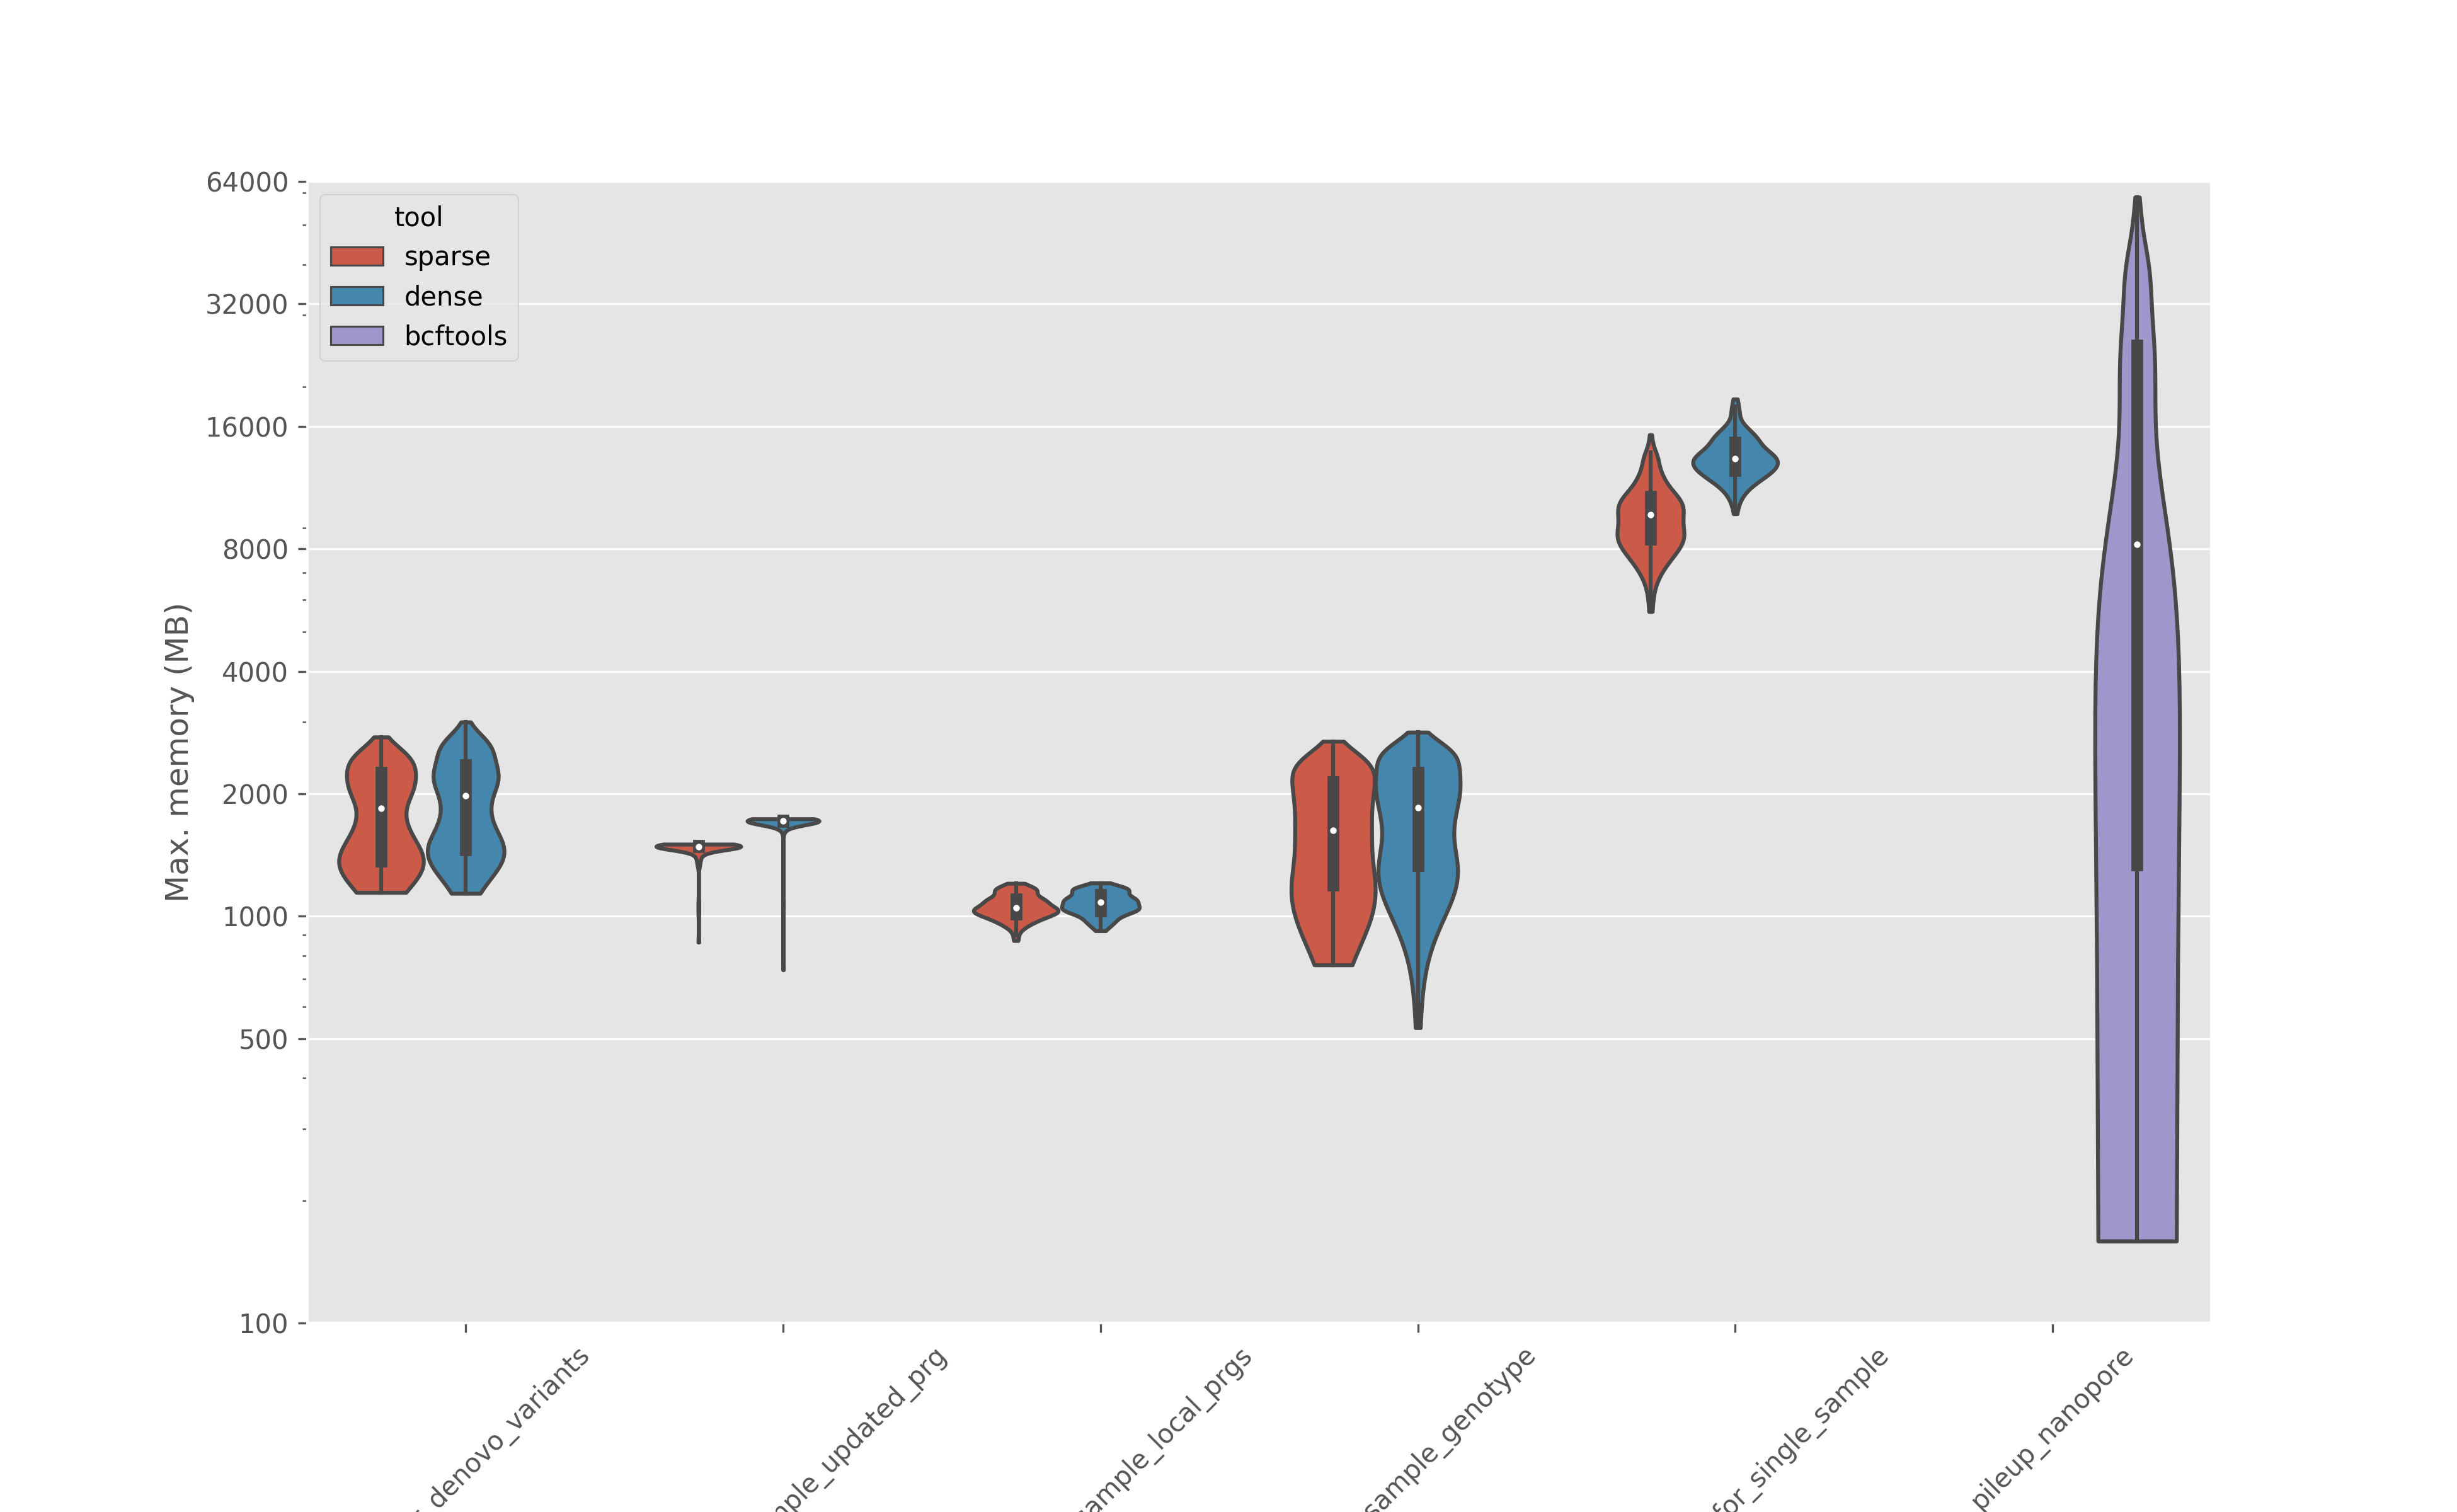
\includegraphics[width=\textwidth]{Chapter2/Figs/max_mem.png}
         \caption{}
         \label{fig:max-mem}
     \end{subfigure}
        \caption{The CPU time (in seconds; y-axis; \textbf{a}) and maximum memory usage (in megabytes; y-axis; \textbf{b}) for each \ont{} variant-calling job. Sparse (red) and dense (blue) refer to \pandora{} steps with the respective density \prg{}. \vrb{bcftools} (purple) only has one step (\vrb{pileup\_nanopore}). The violins represent the distribution of CPU time over all samples. }
        \label{fig:var-comp-perf}
\end{figure}

\subsection{Summary}
\label{sec:var-summary}

In summary, \autoref{fig:prec-recall-filters} shows that our selection of filters for \ont{} variant callers provide precision on-par with Illumina. However, this precision comes at the cost of a loss in recall. The remainder of this chapter explores how the SNP calls from \ont{} can be used for calculate distances between samples, and define putative transmission clusters from these distances. We are especially interested in how similar the pairwise distances are between samples and sequencing modality and whether the same distance thresholds used for Illumina can also be used for \ont{}.

\begin{figure}
\begin{center}
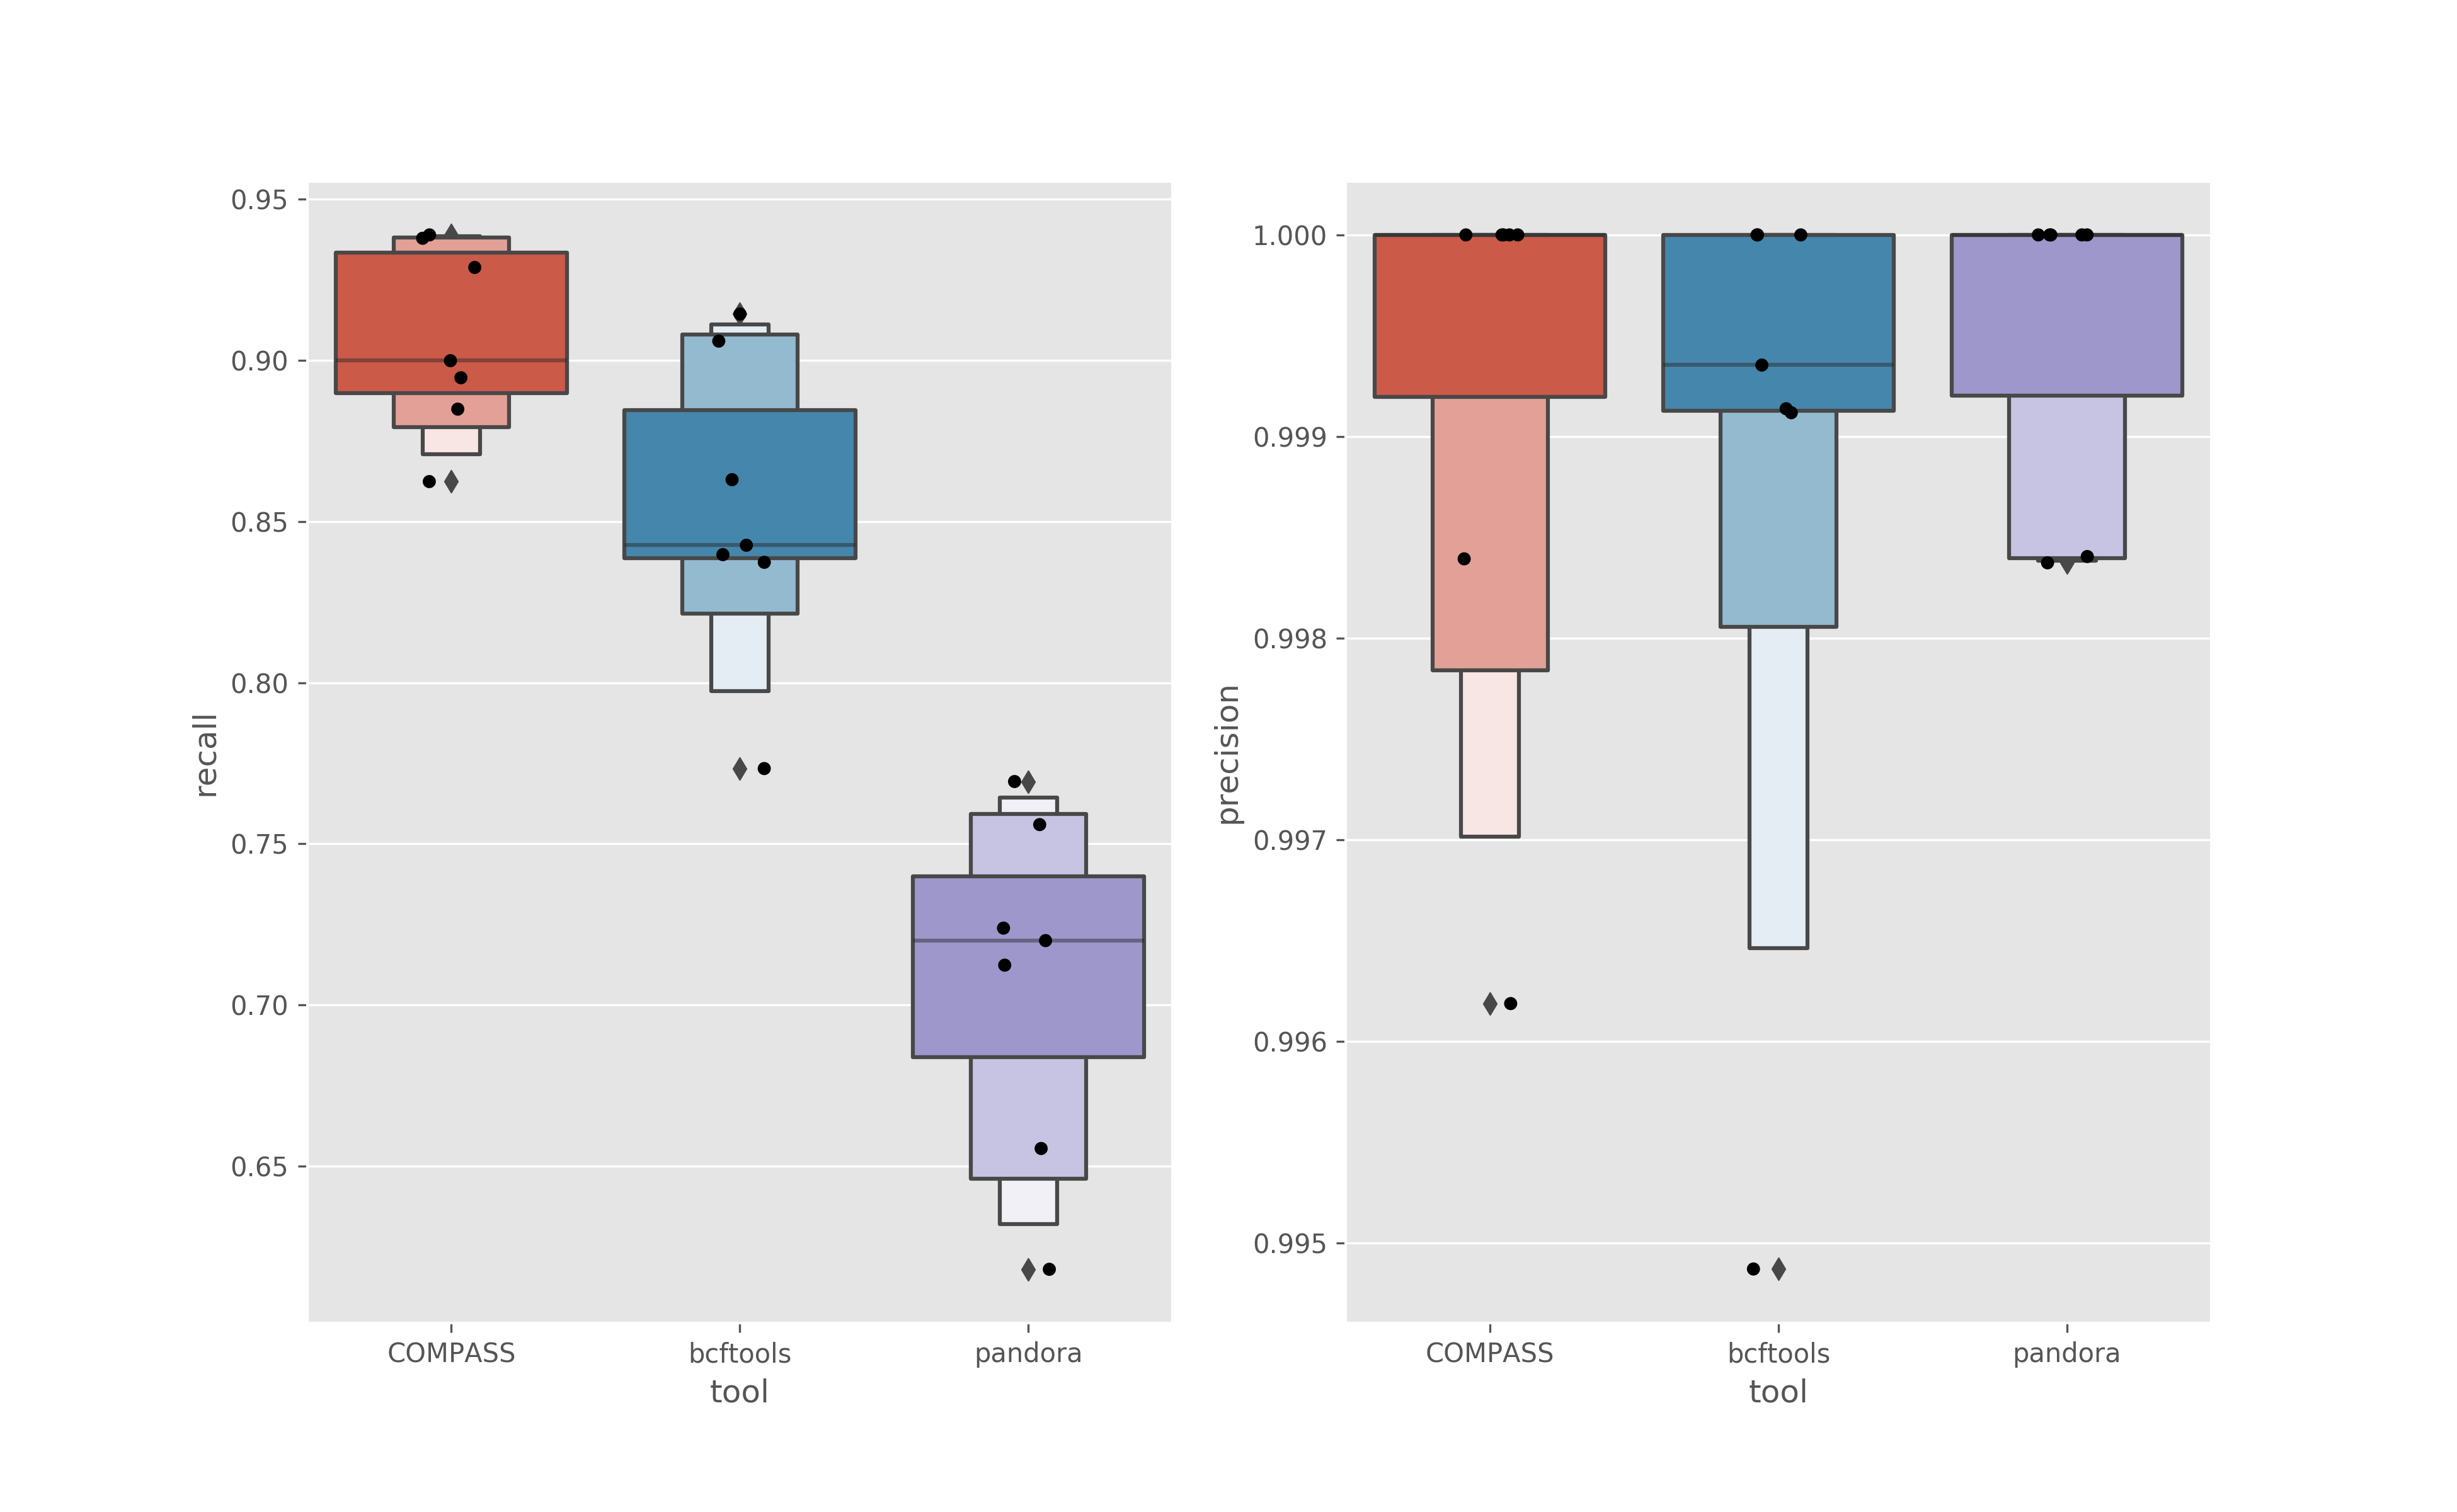
\includegraphics[width=0.9\columnwidth]{Chapter2/Figs/combined-precision-recall-filters-snps.png}
\caption{{Precision (left) and recall (right) of filtered SNPs for COMPASS (red), bcftools (blue), and \pandora{} (purple). Each black point represents one of seven evaluation samples. 
{\label{fig:prec-recall-filters}}%
}}
\end{center}
\end{figure}

%=========================================================================

\section{Pairwise SNP distance comparison for Illumina and \ont{} sequencing data}
\label{sec:snp-dist}

When attempting to infer transmission clusters, the accepted approach is
to define a SNP distance threshold and say that any genomes within this
distance of each other are clustered (possible transmissions). It follows that the SNPs used must
be trusted. Having shown that SNP precision on-par with Illumina can be
achieved with \ont{} data, we investigate the pairwise SNP distance
between samples produced by both sequencing technologies. The intention
here is to determine whether the thresholds typically used for Illumina
data can also be used for Nanopore, or whether adjustments need to be
made.

To determine the distance between samples, we first generate sample consensus sequences. We do this for each variant-caller: COMPASS (Illumina), bcftools (\ont{}), and \pandora{}'s single-sample mode (\ont{}) (not \pandora{}'s multi-sample mode). A consensus sequence is obtained by applying the calls from a given VCF (from \autoref{sec:var-calls}) to the \mtb{} reference genome. We nullify (mark as \vrb{N}) any positions where i) the position failed filtering, ii) the reference genome position does not appear in the VCF file (except for \pandora{} single-sample), iii) the called genotype is null, or iv) the position is within the reference genome mask. All sample consensus sequences for a variant-caller are joined into a single FASTA file and a pairwise distance matrix is calculated using \vrb{snp-dists} (version 0.7.0) \cite{snp-dists}. In the case of \pandora{} \vrb{compare} (multi-sample mode), we cannot follow this approach for generating a consensus sequence and distance matrix, due to the inability to translate the coordinates from a graph to a linear reference. Instead of a consensus sequence, we generate a genotype array by extracting the called genotype for each sample at each site (VCF record). Where a site has failed a filter, we use a genotype value of -2. To calculate the distance between two samples, we compare their genotype arrays; if either sample's genotype is $<0$ (i.e. null or filtered) or the genotypes are the same, we record a distance of 0, otherwise 1. The sum of these comparisons for each genotype is the distance between the two samples.

The pairwise SNP distance relationship can be seen in
\autoref{fig:dotplot}. For a given pair of samples, we
plot their SNP distance, based on the COMPASS (Illumina) variant calls,
against the SNP distance for the same pair, based on the \ont{} variant calls.

All pairwise comparisons between a sample and itself were removed from the visualisation, and only a single value was used for each pair (i.e. we keep sample1 vs. sample2 and discard sample2 vs. sample1 as they are the same). RANSAC Robust Linear Regression \cite{fischler1981}, as implemented in the Python library \vrb{scikit-learn} \cite{scikitlearn}, was used for determining a linear equation and line-of-best fit for the relationship between pairwise Illumina and \ont{} SNP distance.

 If the same thresholds used for Illumina can
also be used for Nanopore, we would expect the distances to be the same
and the bulk of the points in the plot to fall on the dashed, diagonal
identity line. What we see instead is a linear relationship that falls
\emph{under} this identity line - for all \ont{} variant callers. Given the filtered Nanopore
SNP calls made by bcftools and \pandora{} have lower recall than Illumina (see \autoref{sec:var-summary}), this
is expected, as we miss some SNPs found by Illumina.

One important observation though is highlighted by the zoomed inset in
\autoref{fig:dotplot}. As SNP thresholds used for \mtb{}
are generally well below 100 \cite{stimson2019}, it makes more sense to base SNP distance
relationships on those samples that are ``close''. And indeed, when we
zoom in on pairs of samples within 100 (Illumina) SNPs of each other, we
see an association that falls closer to the identity line. Fitting a
linear model to this close subset of pairwise distances, yields a
relationship defined by the equation $y=0.806x+0.593$ for bcftools, $y=0.575x+13.544$ for \pandora{} single-sample, and $y=0.342x+0.765$ for \pandora{} multi-sample.
Replacing $x$ with an Illumina SNP threshold gives the
(predicted) equivalent Nanopore SNP threshold based on these
relationships. For example, at an Illumina SNP threshold of 12, the
linear equation would predict a corresponding bcftools Nanopore SNP distance of
10.

\begin{figure}
\begin{center}
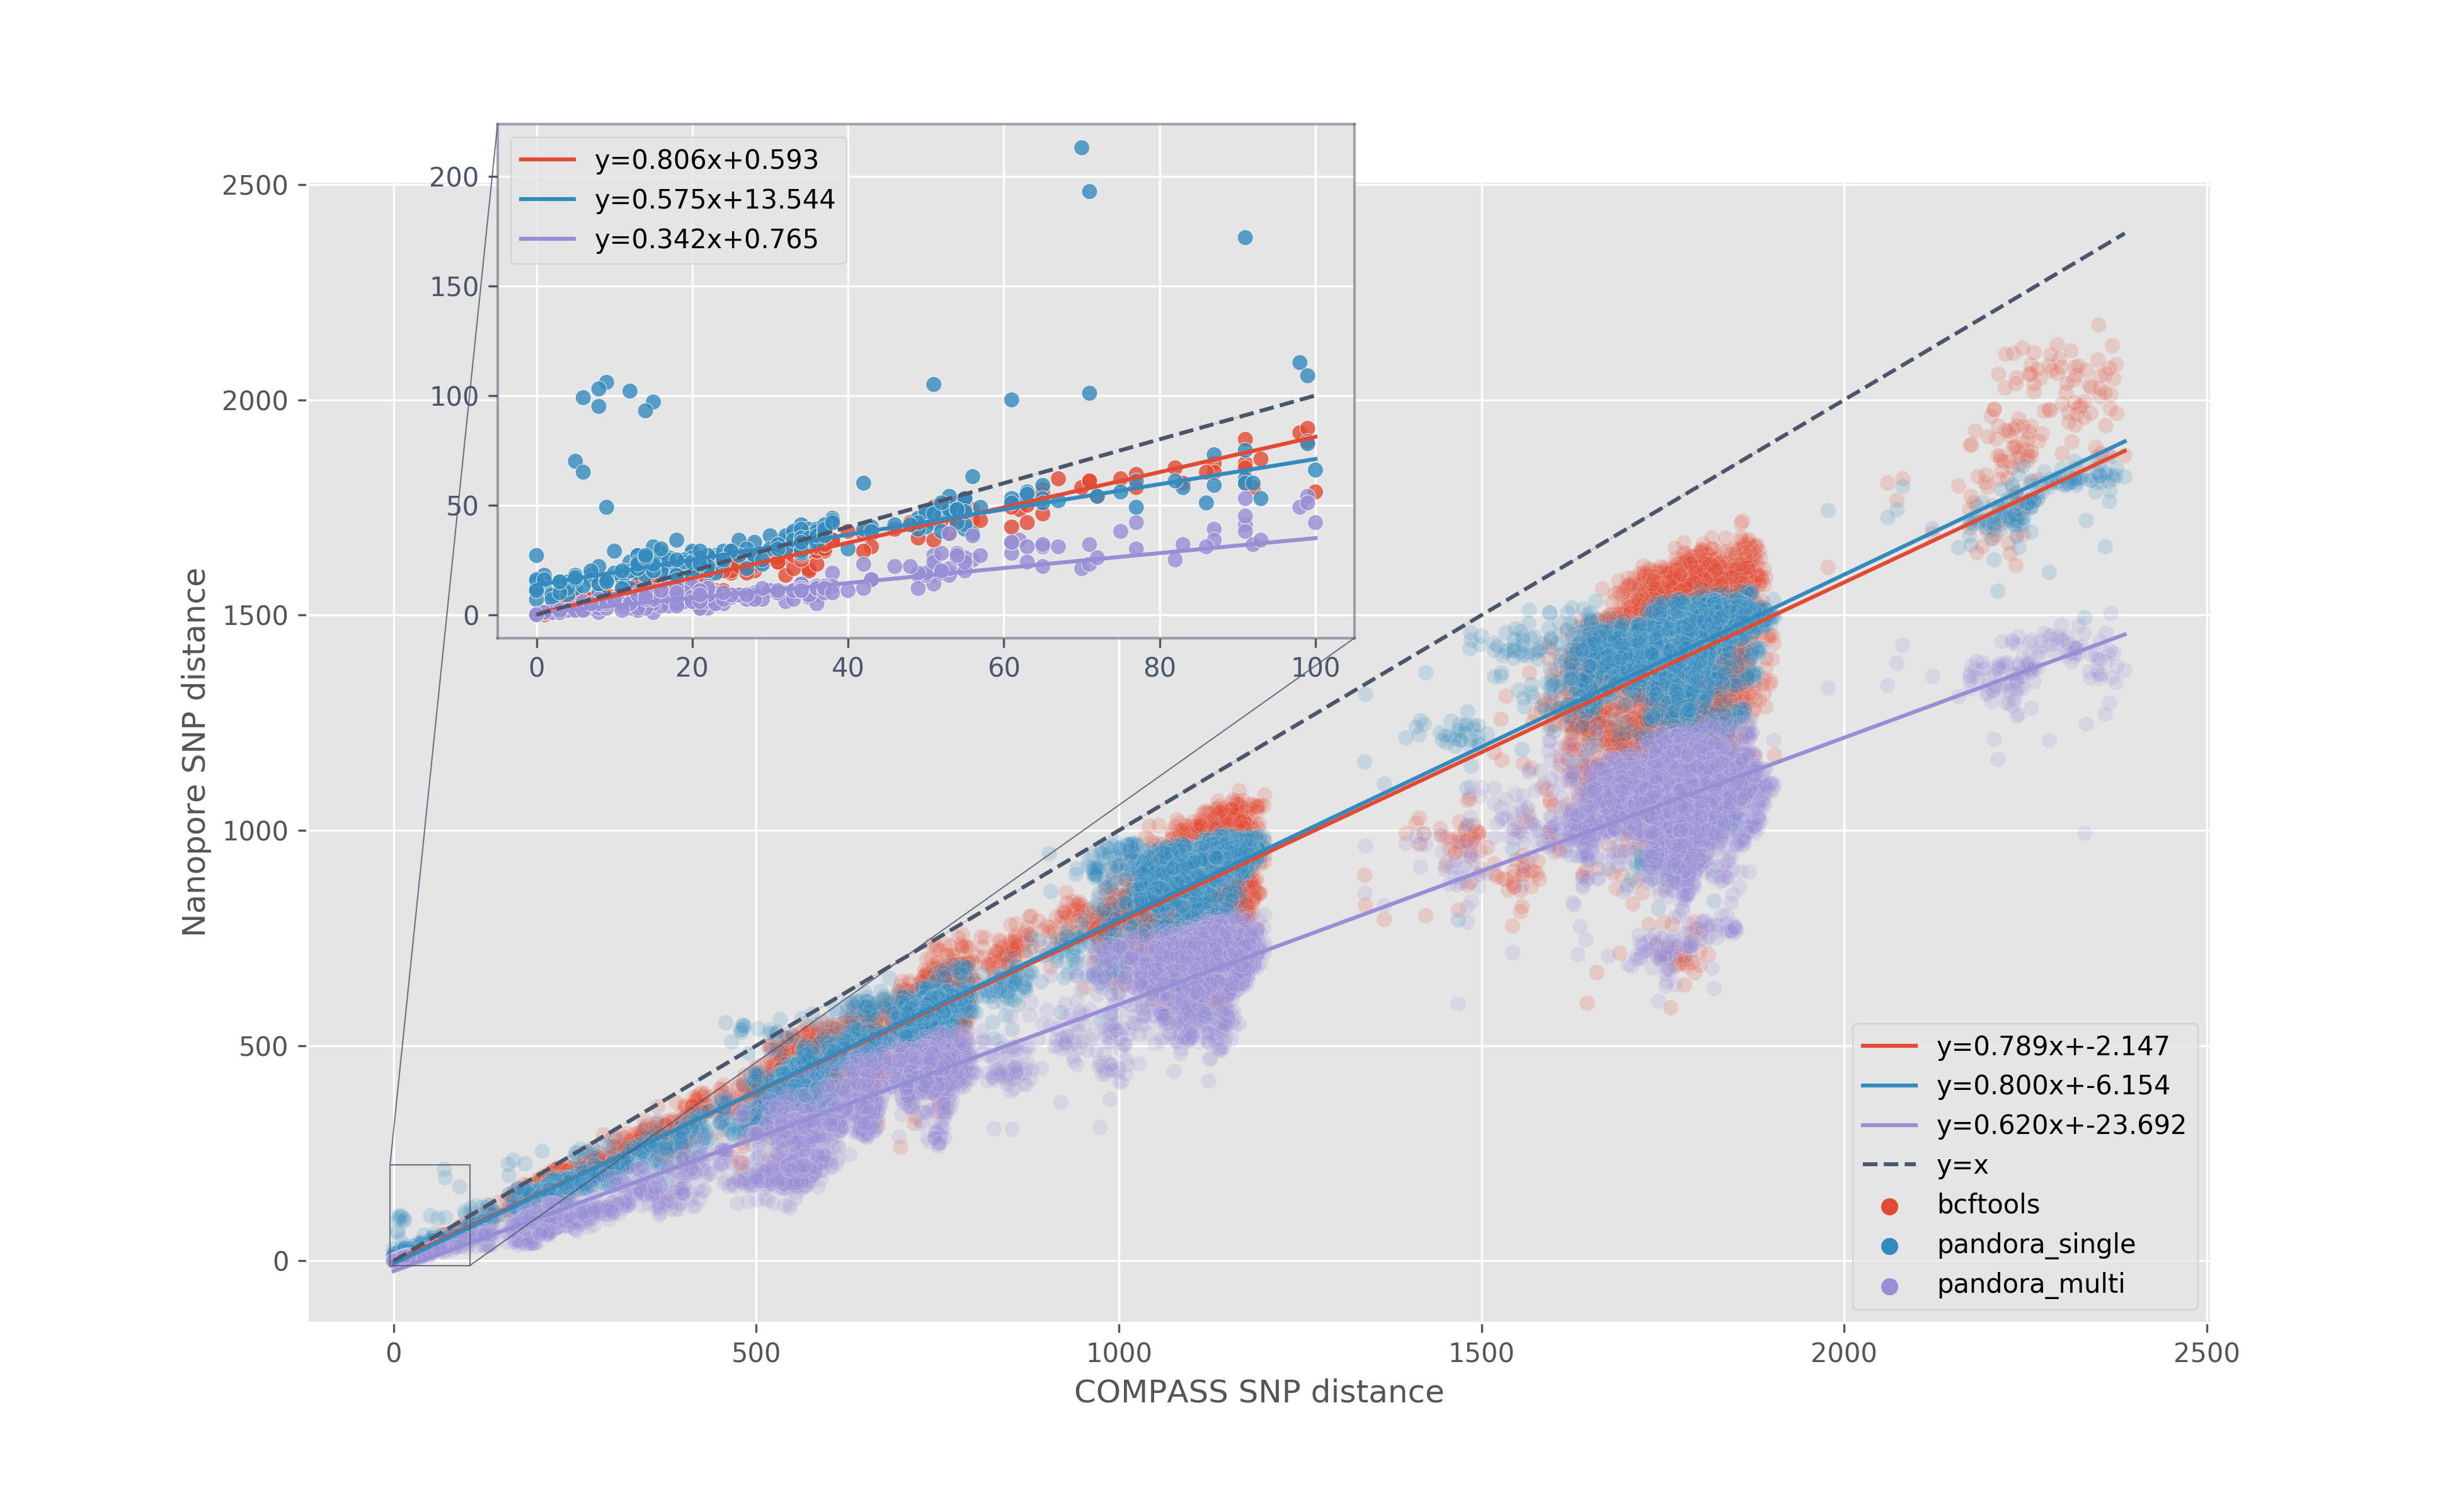
\includegraphics[width=0.90\columnwidth]{Chapter2/Figs/combined-dotplots.png}
\caption{{Pairwise SNP distance relationship between Illumina (COMPASS; x-axis)
and \ont{} (bcftools (red), and \pandora{} single-sample (blue) and multi-sample (purple) mode; y-axis) data. Each point represents the SNP
distance between two samples for the two sequencing modalities. The black, dashed line shows the identity
line (i.e. y=x) and the coloured lines shows the line of best fit based on
the robust linear model fit to the data. The zoomed inset shows all
pairs where the COMPASS distance is~\(\le100\).
{\label{fig:dotplot}}%
}}
\end{center}
\end{figure}

%  see https://github.com/mbhall88/head_to_head_pipeline/issues/61 for a full investigation of the outliers discussed below
In the middle-left of the inset in \autoref{fig:dotplot} a small cluster of \pandora{} single-sample (blue) points can be seen. These have an approximate pairwise \ont{} distance of 100, but \texttildelow 10 for Illumina. Upon further investigation, the cause of the large discprepancy in distance was due to \pandora{} single-sample failing to identify a number of heterozygous calls. Two samples in particular occur as one member in all of the major outlying pairs. 94\% of the false positive differences leading to the large \ont{} distances occur at positions that are filtered due to evidence of heterozygosity in COMPASS. That is, in the Illumina consensus sequence these positions are ignored and do not count as a difference. However, \pandora{} did not have sufficient read depth on both alleles to trigger the FRS filter (see \autoref{sec:pandora-filters}) - leading to a passing variant call that differs from the sample it is being compared with.


The relationship between Illumina and \ont{} distances is indeed linear for all three variant-calling methodologies. While the relationship is not identical (i.e. a distance of 12 for Illumina does not necessarily mean a distance of 12 for \ont{}), we will attempt to use linear models fit to the relationship to infer what \ont{} SNP distance threshold is likely to align with a given Illumina threshold for defining putative transmission clusters.

%=========================================================================

\section{SNP threshold-based \ont{} transmission clustering}
\label{sec:clustering}

It is one thing to look at the relationship between Illumina and
Nanopore pairwise SNP distance, but ultimately the most important
question is: do Nanopore SNPs lead to transmission clusters consistent
with those obtained with Illumina SNPs? To answer this question, we
compare Illumina- and Nanopore-based clusters for{ four
clinically-interesting (Illumina) SNP thresholds -} 0, 2, 5, and 12. 

Selecting a SNP threshold to infer transmission clusters from has seen a
variety of values recommended \cite{stimson2019}. As we seek to show
concordance of \ont{} data with PHE's Illumina-based strategy, we opt
to investigate Illumina threshold values 0, 2, 5, and 12. PHE define two cases as clustered
if they have a SNP distance $\le$ 12 as "\emph{although 12
SNPs represents the maximum SNP difference between 2 isolates for which
epidemiological links have previously been identified
\cite{walker2013} and is a conservative measure for reporting
isolate relatedness}"\cite{phe-tb-england}. Five was likewise selected as
it was found by \cite{walker2013} to indicate membership in a recent
transmission chain. Threshold values 0 and 2 were chosen to provide
insight into the level of granularity possible and is of clinical
interest in certain settings (personal correspondence). For each of these four thresholds, we investigate what corresponding \ont{} SNP distance threshold yields the most similar clustering.

\subsection{Transmission cluster similarity}
\label{sec:cluster-similarity}

We use the distance matrices from \autoref{sec:snp-dist} to infer transmission clusters. In order to cluster samples, for a given SNP threshold $t$, we use only pairs of samples in the distance matrix with a distance $\le t$ to define a graph, $G=(V,E)$, where samples (nodes, $V$) are connected by weighted edges ($E$), with the weight of an edge indicating the distance between the two samples it connects. Clusters are defined as the set of connected components $\{C_1, C_2...C_N\}\in G$, where $N$ is the number of clusters. That is, a cluster (connected component), $C_i$, is a subgraph of $G$ where a path exists between any two samples in $C_i$, but no path exists to any samples in the rest of $G$. With this definition, all clusters have a minimum of two members. \\
To assess how closely \ont{} SNP-based clustering approximates Illumina SNP-based clustering we use a similarity measure on sets, the Tversky Index \cite{tversky1977}. We define the Illumina clustering as $G$ and the \ont{} clustering as $H$ and formulate the Tversky Index as 

\begin{equation}
   TI=\frac{\sum_{n}^{V_G}\frac{\left|C_{n,G}\cap C_{n,H}\right|}{\left|C_{n,G}\cap C_{n,H}\right|+\alpha |C_{n,G}-C_{n,H}|+\beta |C_{n,H}-C_{n,G}|}}{|V_G|}
\end{equation}

where $V_G$ is the set of samples (nodes) in $G$ and $C_{n,G}$ is the cluster in $G$ that sample $n$ is a member of. When $\alpha = 1$ and $\beta=0$ we get the Sample-Averaged Cluster Recall (SACR) and when $\alpha = 0$ and $\beta = 1$ we get the Sample-Averaged Cluster Precision (SACP). SACR states, on average, what proportion of the samples clustered together in $G$ (Illumina) are also clustered together in $H$ (\ont{}) - it is a measure of how many true positives \ont{} retains. Inversely, SACP states, on average, what proportion of the samples clustered together in $H$ are also clustered together in $G$ - it is a measure of how many extra samples \ont{} adds to clusters. \\
SACR and SACP do not inherently account for when $H$ has clusters containing no samples in $G$. In order to quantify any extra clustering by $H$, we characterise the Excess Clustering Rate (XCR) as the proportion of singletons (unconnected nodes) in $G$ are (incorrectly) non-singletons in $H$. We define this as

\begin{equation}
\label{eq:xcr}
    XCR = \frac{|S_G-S_H|}{|S_G|}
\end{equation}

where $S_G$ is the set of singletons in $G$ and $S_H$ is the set of singletons in $H$.

We implement SACR, SACP and XCR calculation in the Python programming language with
the~\texttt{networkx} library \cite{networkx}. For a given threshold,
we create the Illumina clustering (graph), $G$, and the
\ont{} clustering, $H$. For each sample (node)
in $G$, we count the number of samples in its cluster
(neighbours) in both $G$ and $H$. To
determine SACR we divide the number of neighbours by the number of
samples in its cluster in $G$. Likewise, we determine
SACP by dividing the number of neighbours by the number of samples in
the sample's cluster in $H$. Both SACR and SACP are the
mean for all samples in $G$. 

To summarise, for each sample in an Illumina-defined cluster, SACR is the
proportion of samples in its Illumina cluster also in its \ont{}
cluster - averaged over all samples. SACP is the proportion of samples
in its \ont{} cluster also in its Illumina cluster - averaged
over all samples. SACR indicates whether samples have been missed from
Nanopore clustering (false negatives) and SACP reveals if additional
samples are being added to Nanopore clusters (false positives). One
shortcoming of SACR and SACP is they do not account for when the
Nanopore clustering contains clusters where no member of the cluster is
part of an Illumina cluster. To that end, XCR is the proportion of Illumina non-clustered
(singleton) samples that are added to a cluster by Nanopore. An XCR value of 0.1 would
indicate that 10\% of non-clustered samples were actually part of a
cluster in the Nanopore clustering. An illustrated, worked example of these metrics can be found in \autoref{app:cluster-example}.

Of the metrics outlined above, our major focus is SACR as missing samples from clusters is of particular concern for public health authorities.

\subsection{Evaluating \ont{} transmission clusters}

\subsubsection{bcftools}
\label{sec:bcftools-clustering}

For the four Illumina SNP distance thresholds of interest - 0, 2, 5, and 12 - the corresponding bcftools thresholds we use are 0, 2, 5, and 11. We chose to forego the model-based predicted thresholds and instead use the hand-picked ones based on the analysis in \autoref{app:dist-sweep}.

\autoref{fig:bcftools-clusters} is a visualisation of these
clustering results for bcftools. The graphs depict the true (Illumina/COMPASS) clusters for each SNP threshold. The inner and outer colours of each node
represent the SACR and SACP values, respectively, for the cluster it is a member of.

The bcftools clustering results are summarised in \autoref{tab:bcftools-cluster-summary} for all four SNP thresholds analysed. Of note, bcftools
achieves a SACR of 1.0 at all thresholds - meaning \ont{} does not miss any samples from
clustering. At the SNP threshold of 2, bcftools clustering only differed from Illumina by the addition of one sample to a cluster of three. 
SNP threshold 5 had the highest XCR (0.057), due to two new clusters of size 2 and 3, and the addition of 2 singleton samples to a cluster of 5. 
The lowest SACP was at threshold 12. This is explained by two cases of a cluster of 2 being added to a larger cluster and 3 singletons being added to existing clusters. 

\begin{figure}
\begin{center}
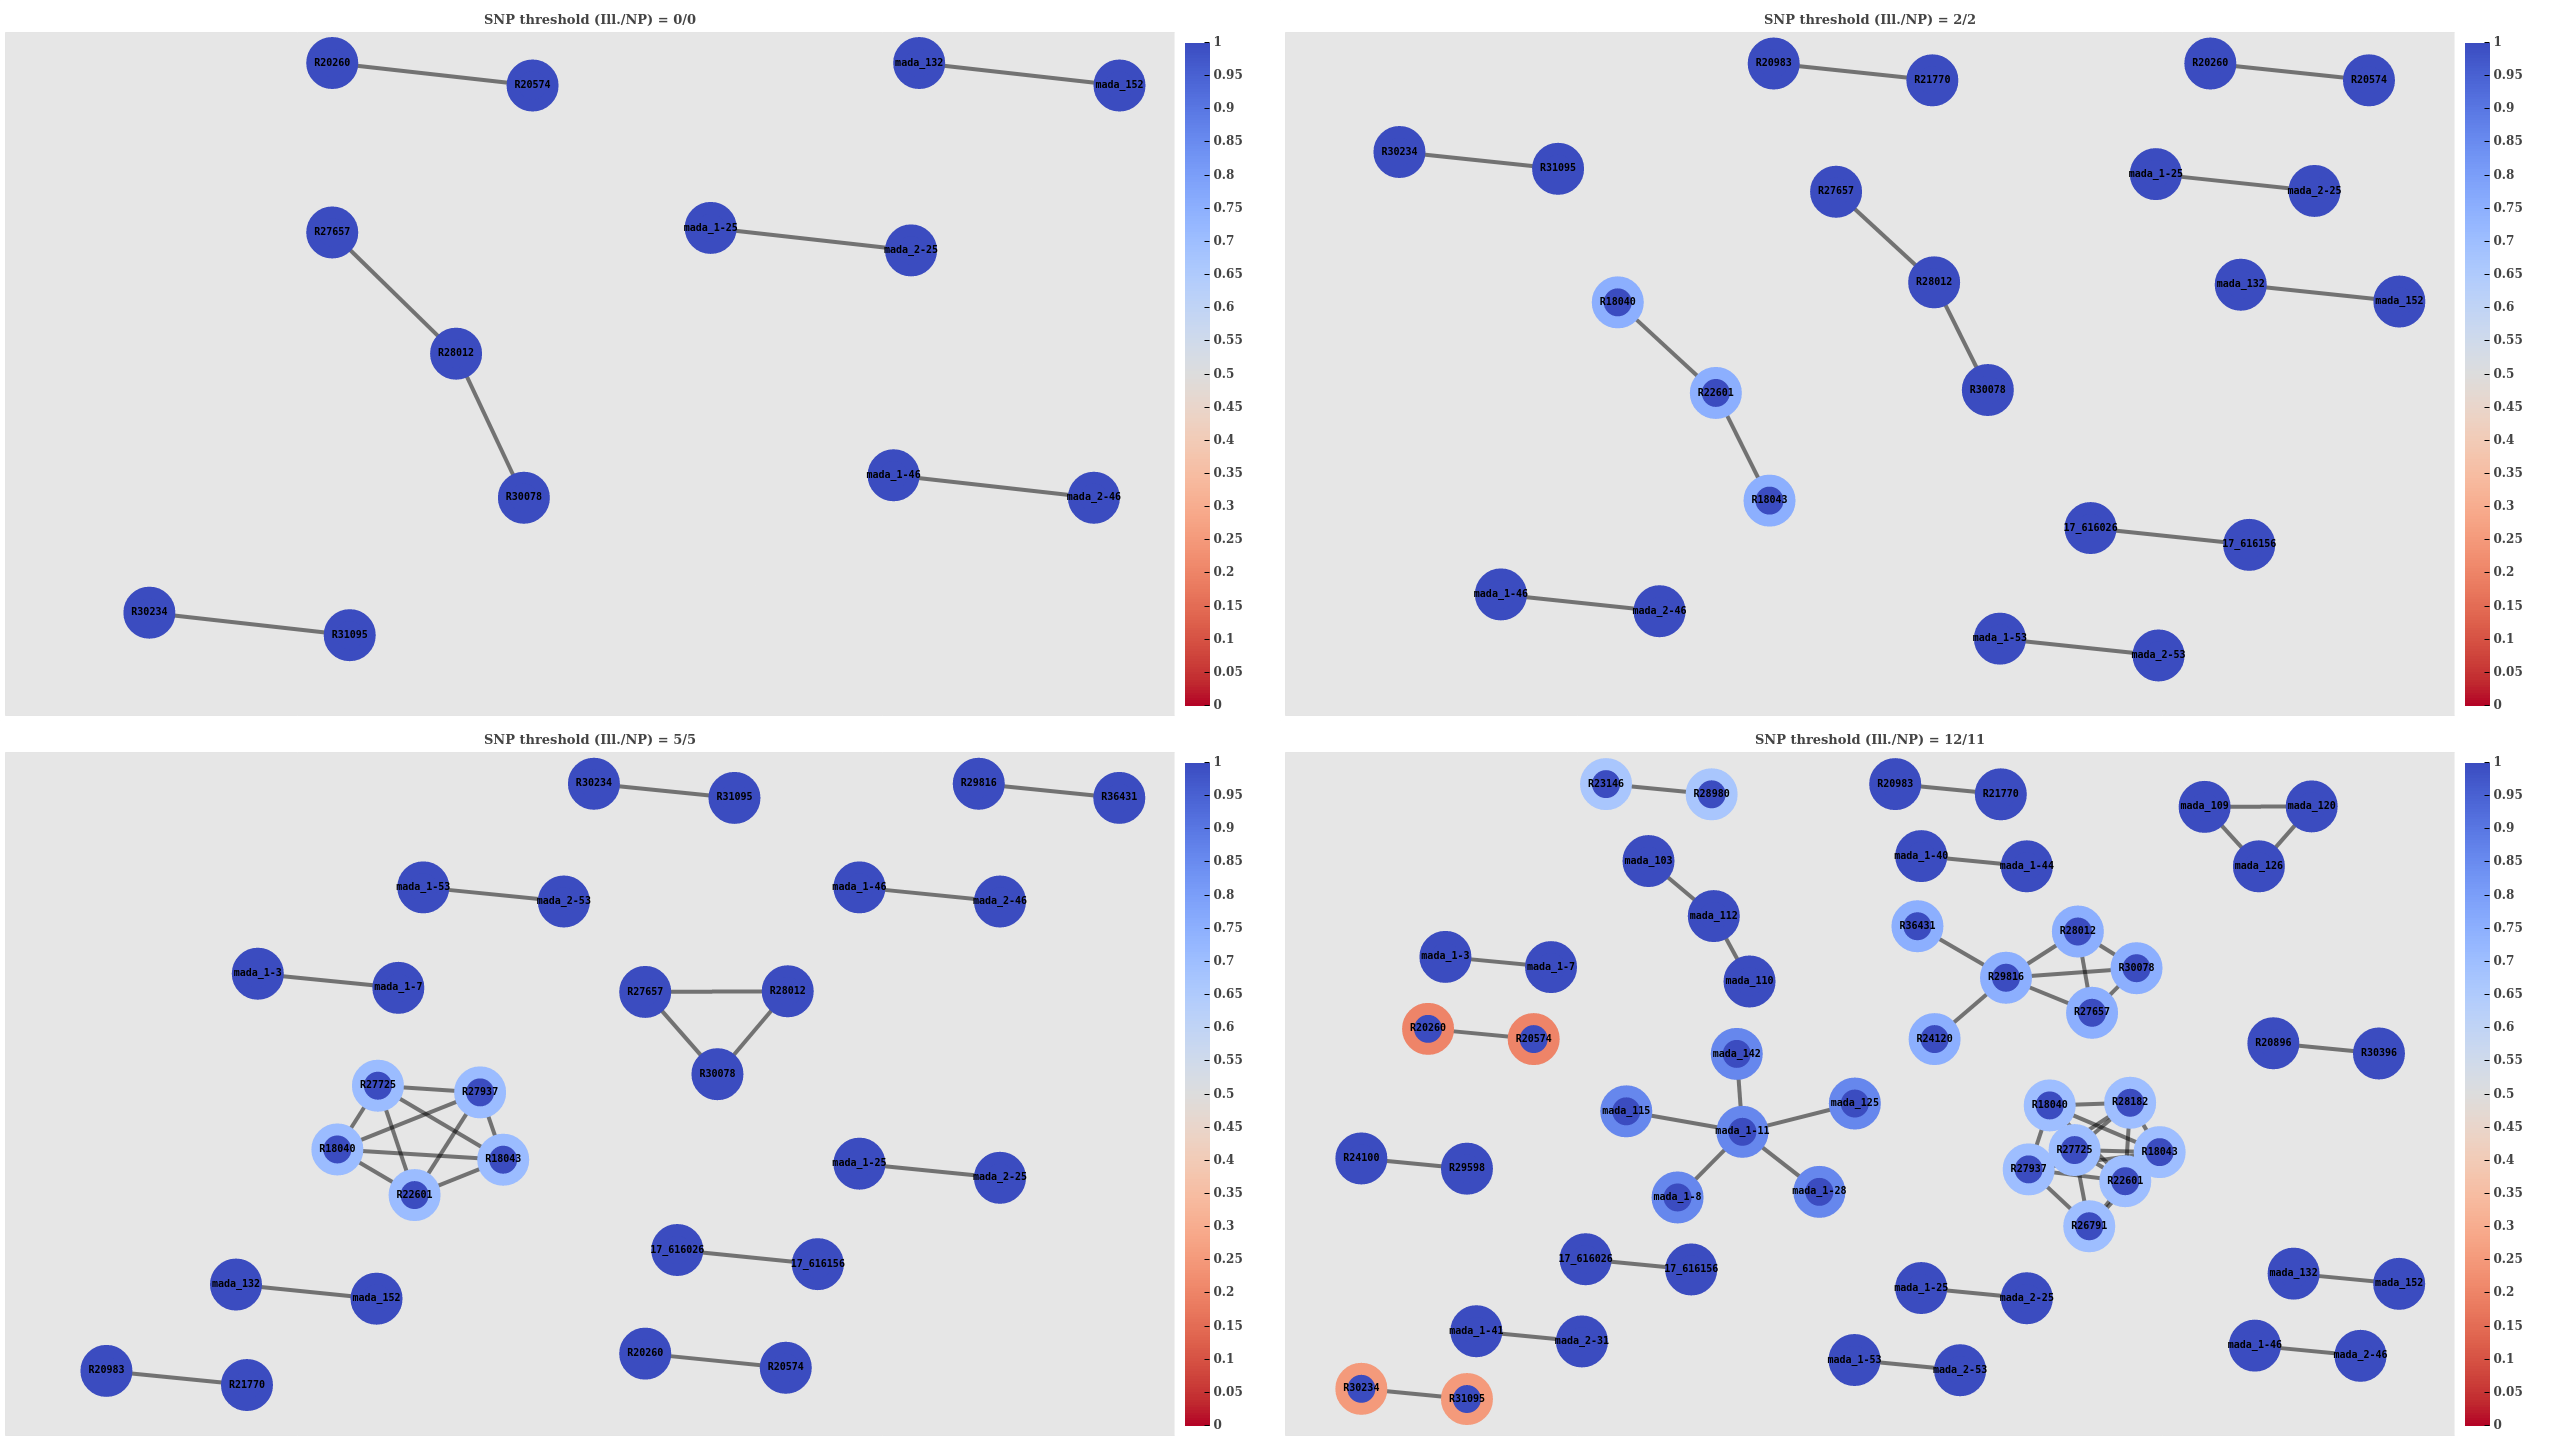
\includegraphics[width=0.90\columnwidth]{Chapter2/Figs/bcftools_clusters.png}
\caption{{Agreement of Illumina and bcftools (\ont{}) transmission clustering at SNP
thresholds 0 (top-left), 2 (top-right), 5 (bottom-left) and 12 (bottom-right). The title of
each subplot indicates the Illumina (Ill.) and Nanopore (NP) threshold
used when clustering. Samples (nodes) are connected when the SNP
distance between them is less than or equal to the relevant threshold.
The inner and outer colours for each node indicates the SACR and SACP
values, respectively, for the cluster it is a part of. The
Illumina-based clustering is shown.
{\label{fig:bcftools-clusters}}%
}}
\end{center}
\end{figure}

\begin{table}
\centering
\begin{tabular}{llll}
Threshold & SACR & SACP  & XCR           \\
\hline
0         & 1.0  & 1.0   & 0.015 (2/137) \\
\hline
2         & 1.0  & 0.966 & 0.008 (1/128) \\
\hline
5         & 1.0  & 0.949 & 0.057 (7/122) \\
\hline
12 (11)       & 1.0  & 0.845 & 0.031 (3/97) 
\end{tabular}
\caption{Summary of bcftools clustering metrics for four (Illumina) SNP distance thresholds. The threshold(s) in parentheses are the \ont{} equivalent threshold used. The fractions in parentheses for XCR indicate the underlying numbers. SACR=sample-averaged cluster recall; SACP=sample-averaged cluster precision; XCR=excess clustering rate.}
\label{tab:bcftools-cluster-summary}
\end{table}

\subsubsection{\pandora{} single-sample}

For \pandora{} single-sample we also chose to use the hand-picked SNP distance thresholds from analysis in \autoref{app:dist-sweep}. These are 16, 18, 18, and 27 for the Illumina thresholds of interest 0, 2, 5, and 12 respecitvely. The clustering results for each of these thresholds are summarised in \autoref{tab:map-cluster-summary} and visualised in \autoref{fig:map-clusters}. At no threshold was \pandora{} single-sample clustering able to achieve perfect SACR, SACP or XCR. In particular, all thresholds had a SACP value less than 0.69 and an XCR greater than 0.11. Taken together, these outline the fact that there were quite a lot of singletons that were erroneously clustered and many clusters joined. In large part, this is expected due to the much wider spread of distances along the y-axis for \pandora{} single-sample in the inset of \autoref{fig:dotplot} when compared to bcftools of \pandora{} multi-sample. Although the SACR values are not as low as the SACP, we place a higher value on them. The nodes with red(ish) outer circles in \autoref{fig:map-clusters} highlight clusters where samples have been missed.

\begin{figure}
\begin{center}
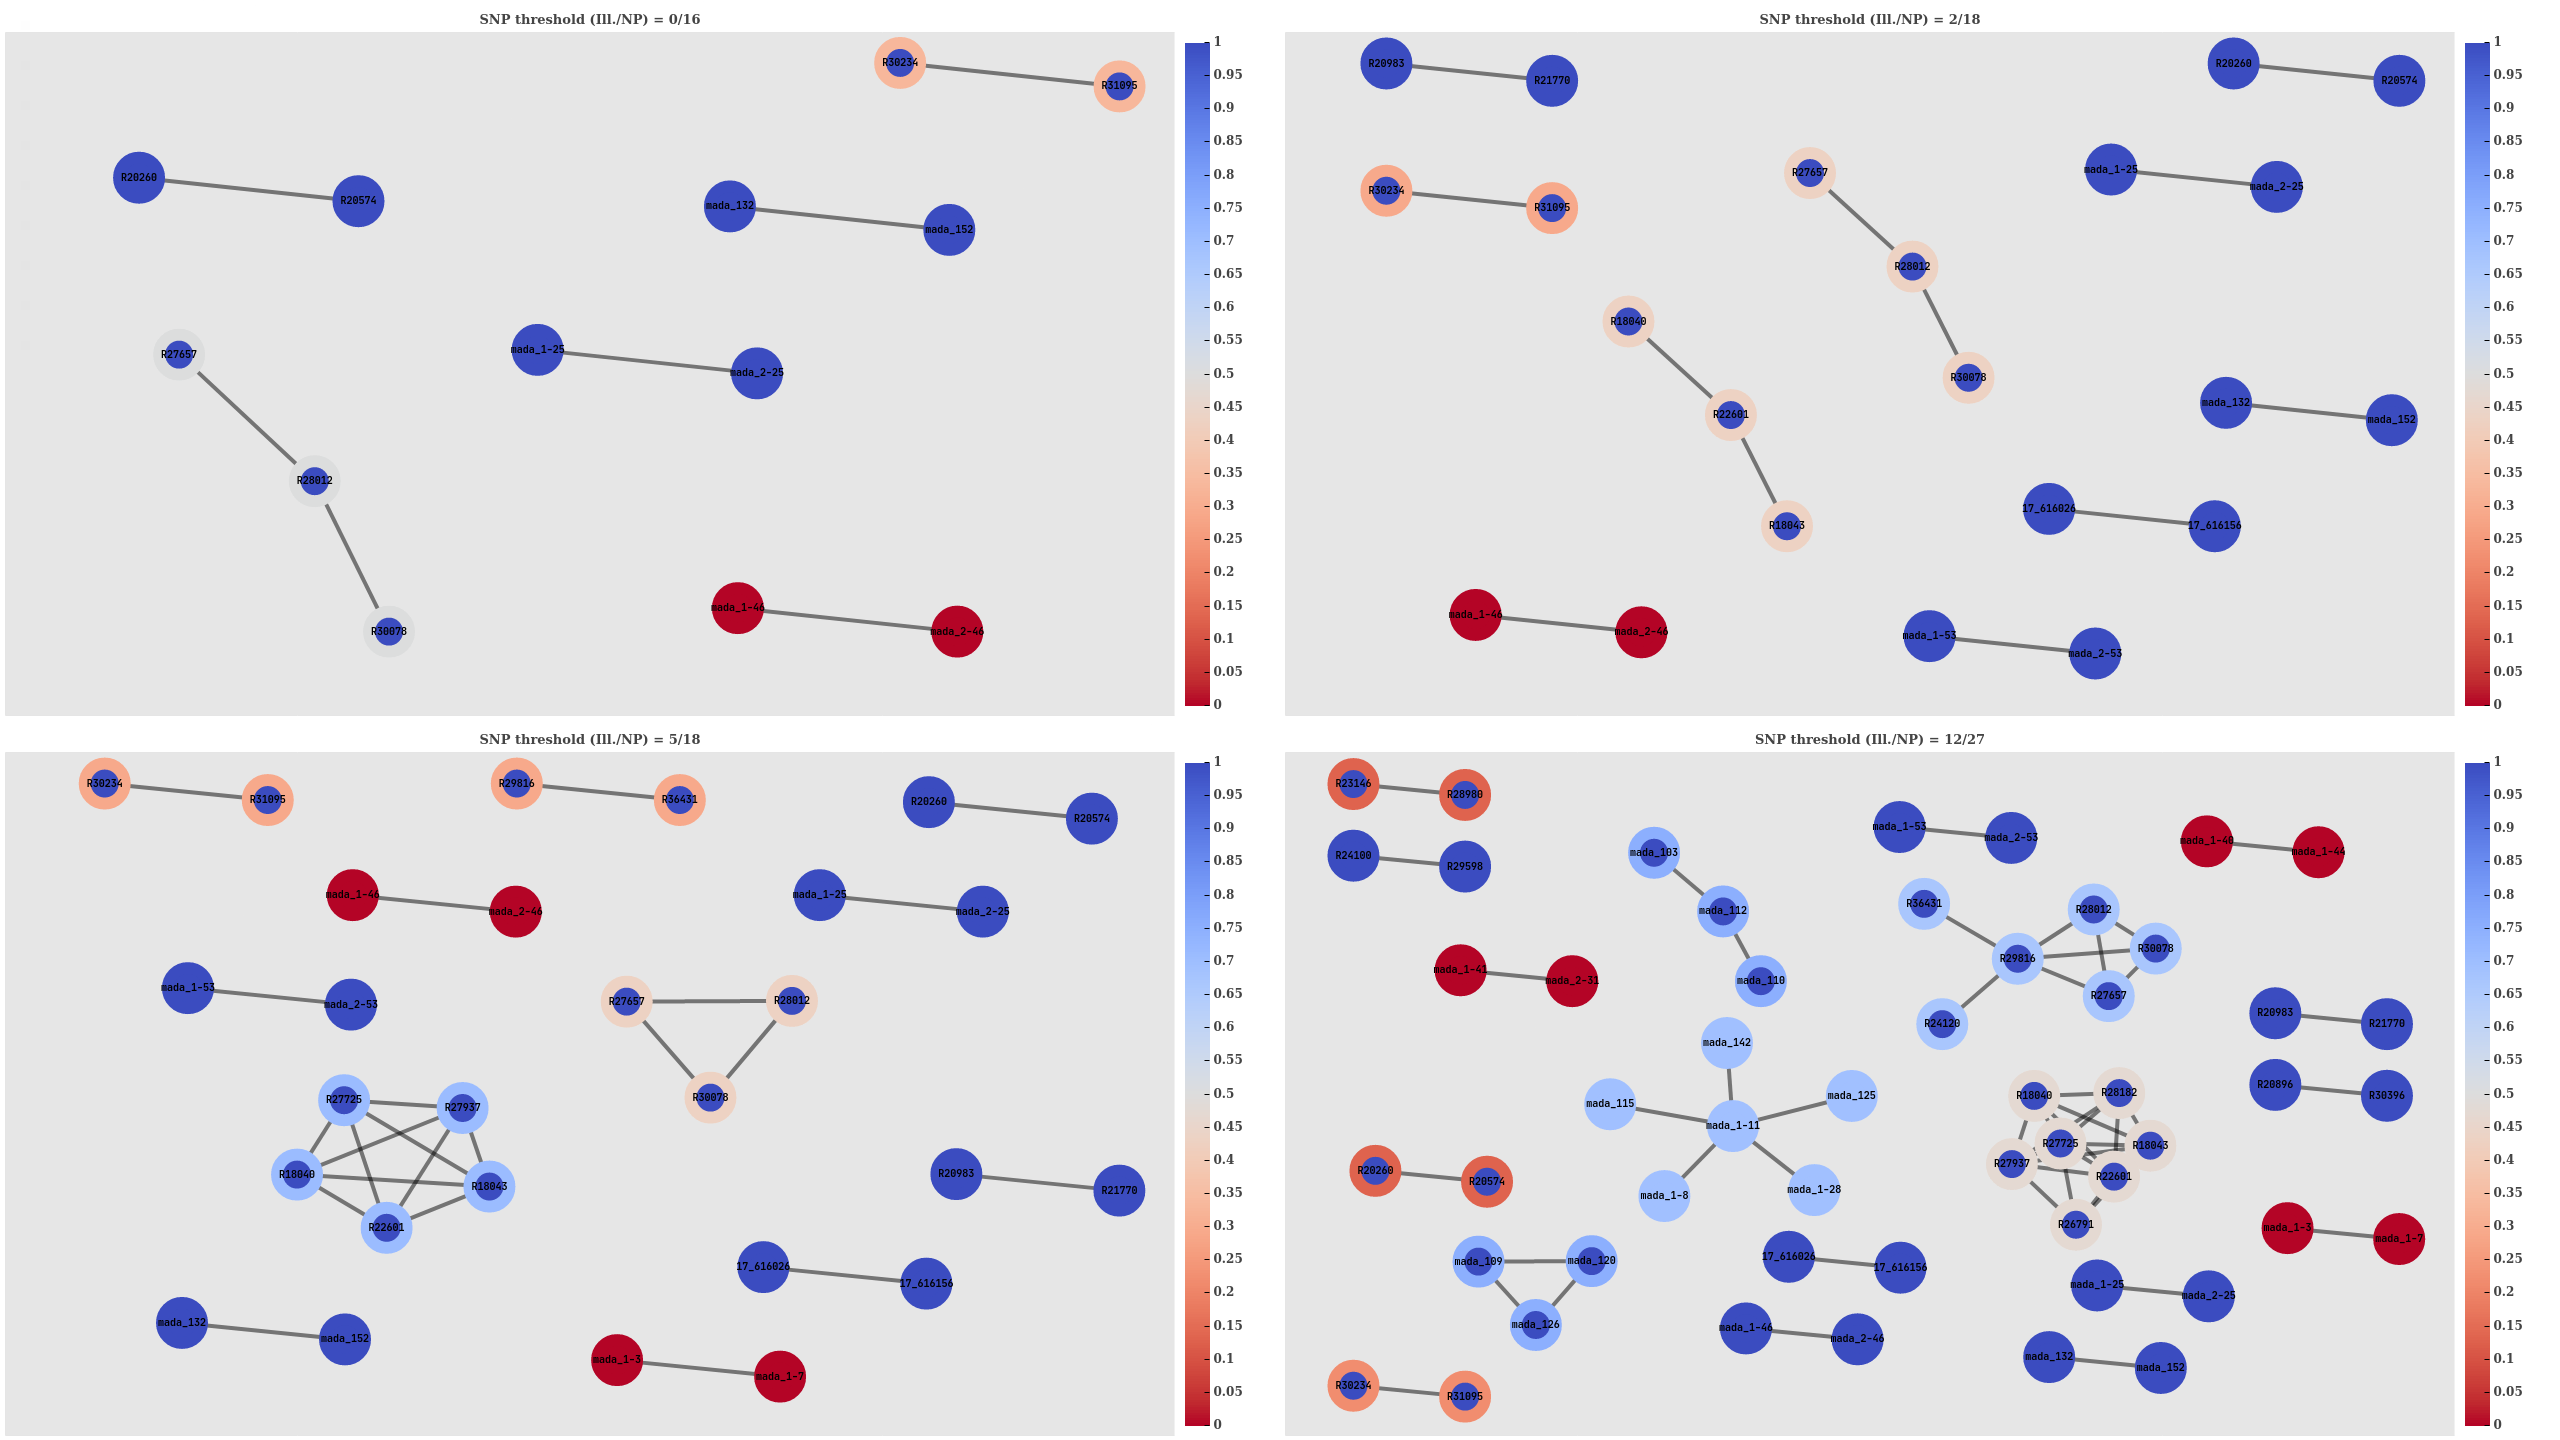
\includegraphics[width=0.90\columnwidth]{Chapter2/Figs/pandora_map_clusters.png}
\caption{{Agreement of Illumina and \pandora{} single-sample (\ont{}) transmission clustering at SNP
thresholds 0 (top-left), 2 (top-right), 5 (bottom-left) and 12 (bottom-right). The title of
each subplot indicates the Illumina (Ill.) and Nanopore (NP) threshold
used when clustering. Samples (nodes) are connected when the SNP
distance between them is less than or equal to the relevant threshold.
The inner and outer colours for each node indicates the SACR and SACP
values, respectively, for the cluster it is a part of. The
Illumina-based clustering is shown.
{\label{fig:map-clusters}}%
}}
\end{center}
\end{figure}

\begin{table}
\centering
\begin{tabular}{llll}
Threshold & SACR  & SACP  & XCR            \\
\hline
0 (16)    & 0.846 & 0.628 & 0.146 (20/137) \\
\hline
2 (18)    & 0.909 & 0.688 & 0.141 (18/128) \\
\hline
5 (18)    & 0.857 & 0.643 & 0.115 (11/122) \\
\hline
12 (27)   & 0.852 & 0.621 & 0.124 (12/97)  
\end{tabular}
\caption{Summary of \pandora{} single-sample clustering metrics for four (Illumina) SNP distance thresholds. The threshold(s) in parentheses are the \ont{} equivalent threshold used. The fractions in parentheses for XCR indicate the underlying numbers. SACR=sample-averaged cluster recall; SACP=sample-averaged cluster precision; XCR=excess clustering rate.}
\label{tab:map-cluster-summary}
\end{table}

\subsubsection{\pandora{} multi-sample}

The SNP thresholds we use for \pandora{} multi-sample clustering are 0, 1, 3, and 7. The results of this clustering are summarised in \autoref{tab:compare-cluster-summary} and visualised in \autoref{fig:compare-clusters}. One important result is that unlike the single-sample approach of \pandora{}, the multi-sample mode leads to perfect SACR across all thresholds. Additionally, the clustering at the threshold of 0 perfectly mirrors Illumina. At a threshold of 2, there was one singleton added to an otherwise perfect cluster and 2 additional clusters of size 2. At thresholds 5 and 12 there were a number of clusters joined into larger ones and some additions of singletons to existing clusters, along with new clusters.

\begin{figure}
\begin{center}
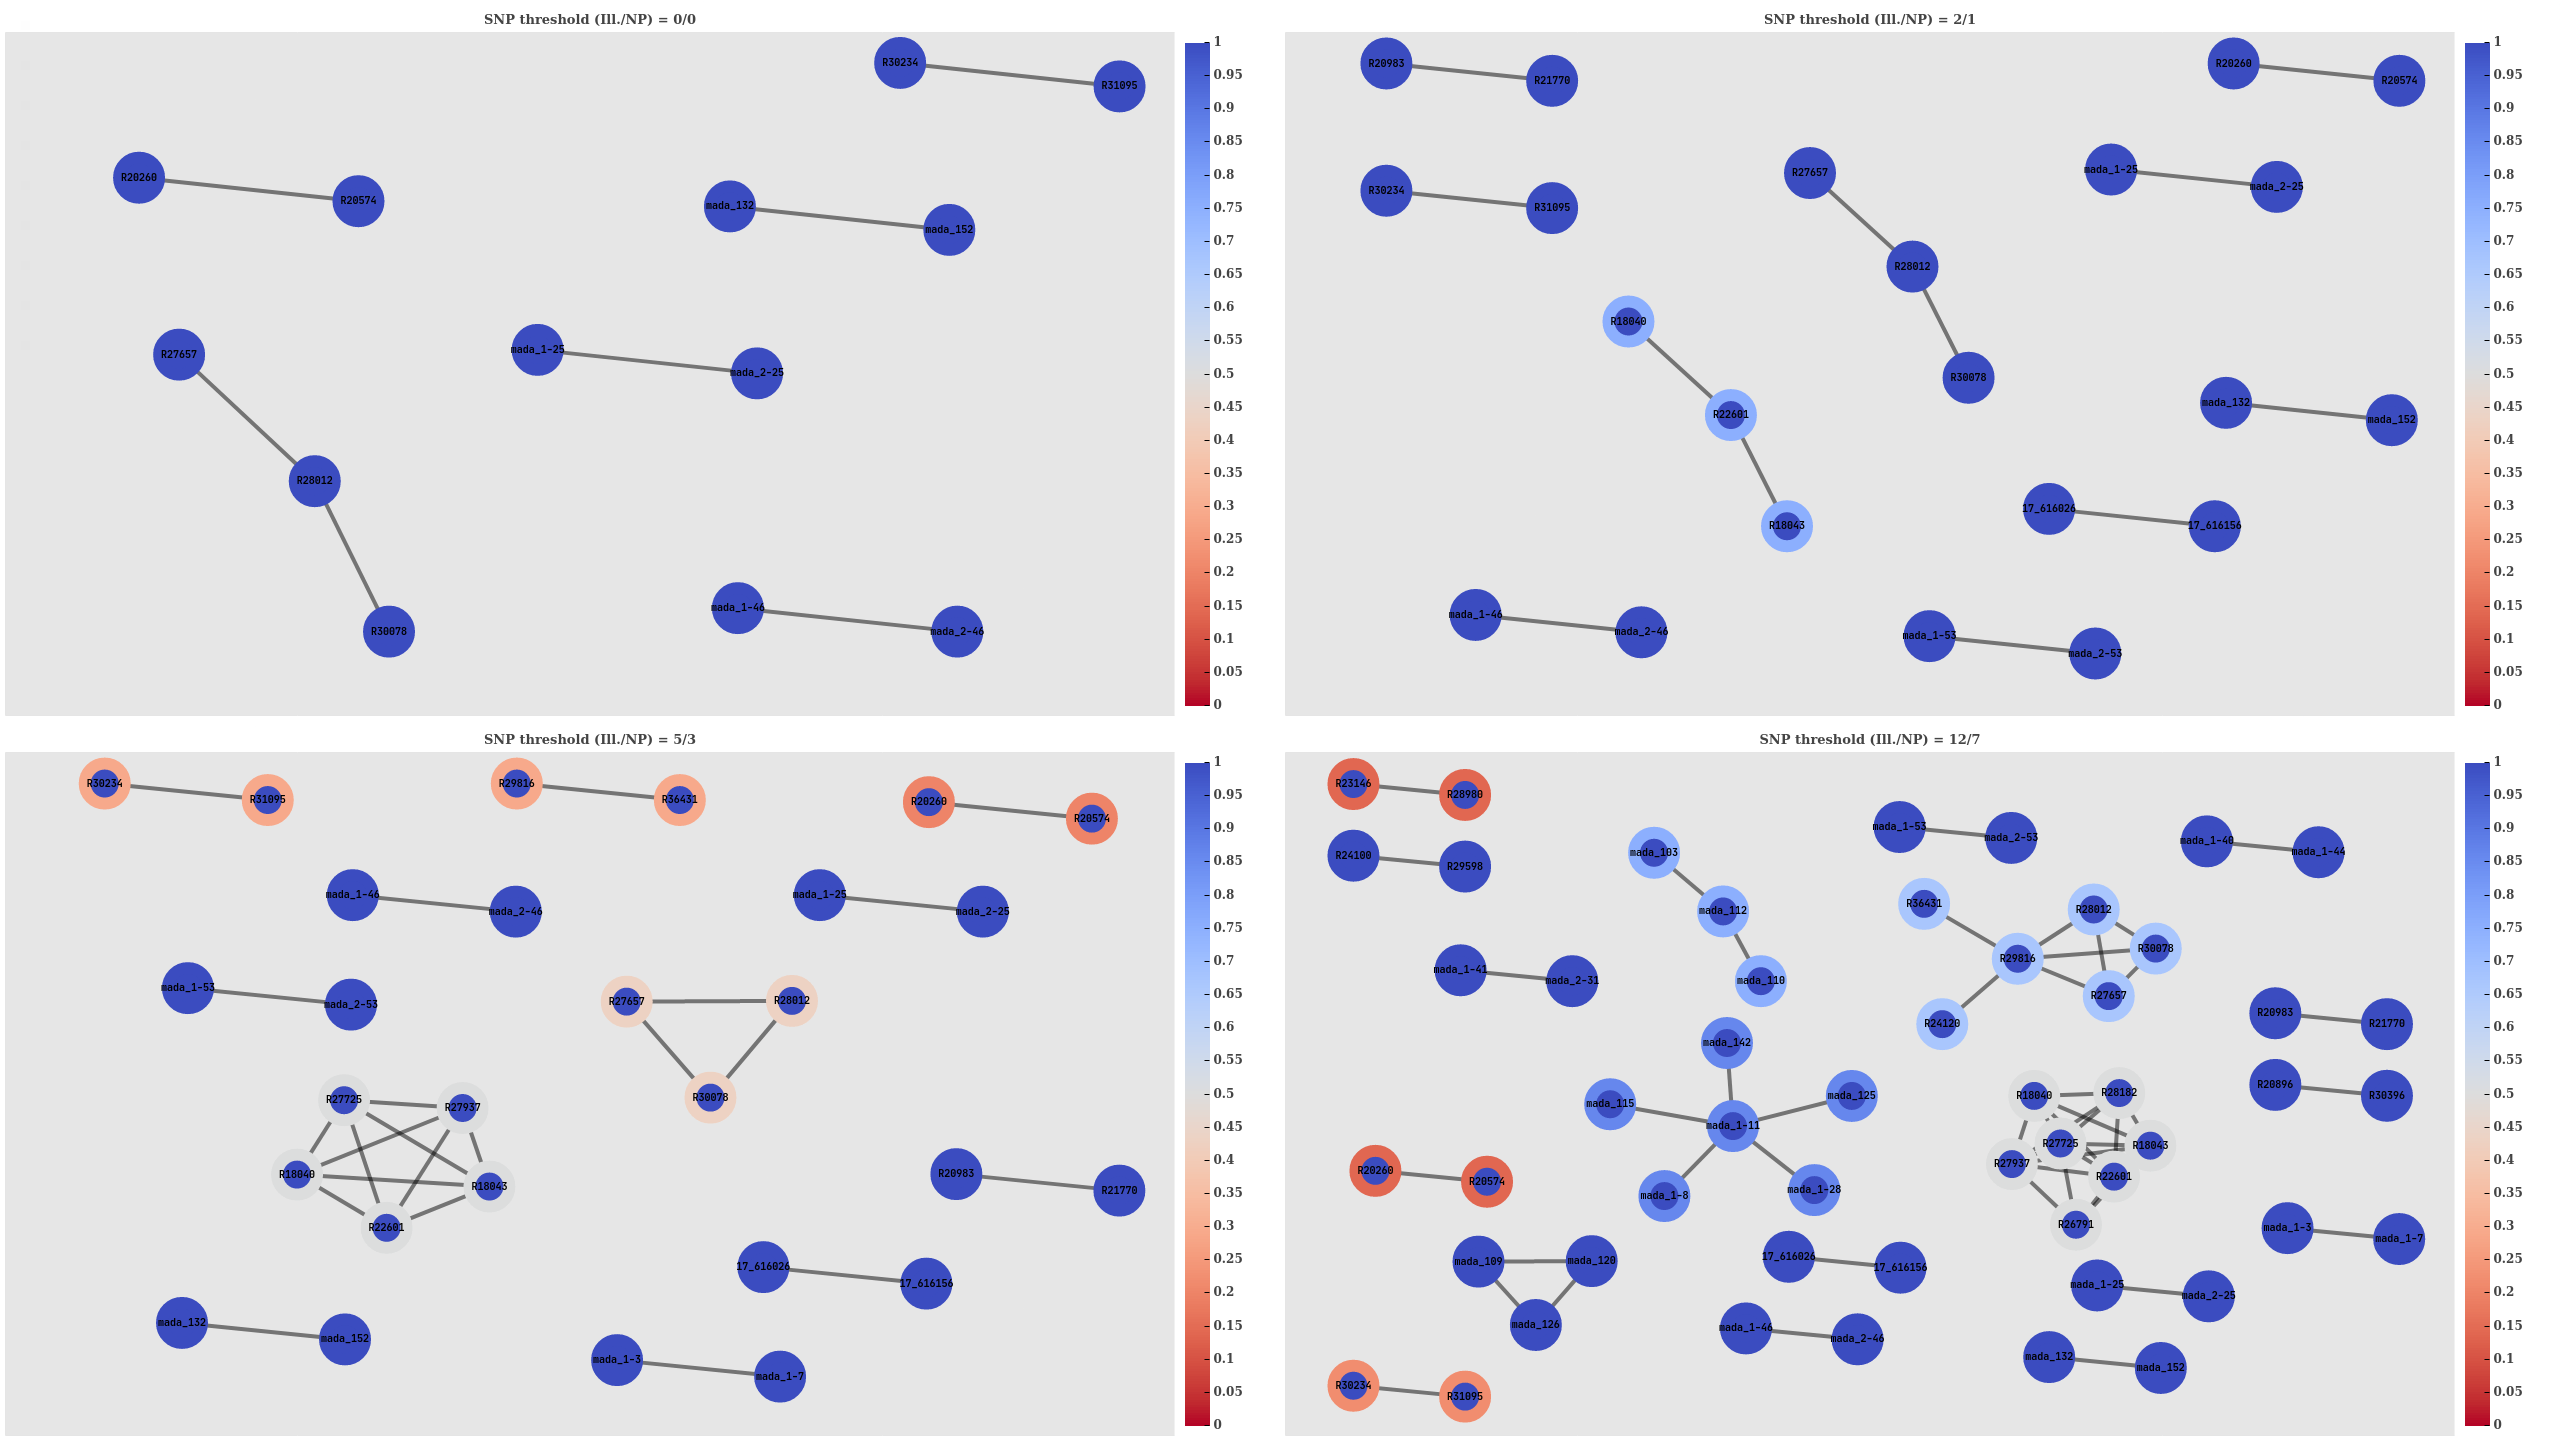
\includegraphics[width=0.90\columnwidth]{Chapter2/Figs/pandora_compare_clusters.png}
\caption{{Agreement of Illumina and \pandora{} multi-sample (\ont{}) transmission clustering at SNP
thresholds 0 (top-left), 2 (top-right), 5 (bottom-left) and 12 (bottom-right). The title of
each subplot indicates the Illumina (Ill.) and Nanopore (NP) threshold
used when clustering. Samples (nodes) are connected when the SNP
distance between them is less than or equal to the relevant threshold.
The inner and outer colours for each node indicates the SACR and SACP
values, respectively, for the cluster it is a part of. The
Illumina-based clustering is shown.
{\label{fig:compare-clusters}}%
}}
\end{center}
\end{figure}

\begin{table}
\centering
\begin{tabular}{llll}
Threshold & SACR  & SACP  & XCR            \\
\hline
0        & 1.0 & 1.0 & 0.0 (0/137) \\
\hline
2 (1)    & 1.0 & 0.966 & 0.039 (5/128) \\
\hline
5 (3)    & 1.0 & 0.690 & 0.090 (11/122) \\
\hline
12 (7)   & 1.0 & 0.772 & 0.103 (10/97)  
\end{tabular}
\caption{Summary of \pandora{} multi-sample clustering metrics for four (Illumina) SNP distance thresholds. The threshold(s) in parentheses are the \ont{} equivalent threshold used. The fractions in parentheses for XCR indicate the underlying numbers. SACR=sample-averaged cluster recall; SACP=sample-averaged cluster precision; XCR=excess clustering rate.}
\label{tab:compare-cluster-summary}
\end{table}

\subsection{Summary}
\label{sec:cluster-summary}

The results presented in this section show that when using bcftools for variant calling \ont{} is capable of producing transmission clusters with a high degree of similarity to Illumina. Most importantly, no samples deemed part of a cluster by Illumina were missed by bcftools. We have also shown that the Illumina SNP thresholds of 0, 2, and 5 are also valid for \ont{} variant calls from bcftools and the threshold of 12 needs only to be reduced to 11. 
We also invesigated whether the genome graph method of \pandora{} could be used to produce accurate transmission clusters. While the single-sample approach did not yield particularly good results, the multi-sample mode showed promise. For all SNP thresholds assessed, \pandora{}'s multi-sample method did not miss any samples from clustering. The SACP values for thresholds 0 and 2 were as good as those from bcftools, but at thresholds 5 and 12 \pandora{} did not perform as well. 

%=========================================================================

\section{Transmission clusters with mixed Illumina and \ont{} data}

Having established that Illumina-defined transmission clusters can be
confidently recreated with \ont{} data, we turn to the question of whether the same holds true when mixing Illumina and
\ont{} data. Being able to deduce transmission clusters from a mixture of sequencing
modalities would allow greater integration across datasets from various
sources and prevent laboratories from being locked into any one
sequencing technology. As the uptake of Nanopore sequencing increases it seems
inevitable there will be cases where comparisons between these
sequencing modalities is necessary. To address this question we simulate
varying degrees of \ont{}/Illumina mixtures and look at how this impacts
clustering. To this end, we investigate what the impact (if any) of combining
Illumina and \ont{} datasets has on SACR, SACP and XCR (see \autoref{sec:cluster-similarity} for definitions). For the \ont{} data, we use the bcftools distance matrices as they were shown to be the most concordant with Illumina (\autoref{sec:cluster-summary}).

Firstly, we get a sense for how comparable the distances are likely to
be but looking at the "self-distance" for each sample - the distance
between a sample's Illumina and \ont{} data. 
As the sequencing data originates from the same source we
know the self-distance for any sample \emph{should} be 0. However, we
also know there are major technological differences between Illumina and
Nanopore, so it is wise to check just how similar they are.
We plot these self-distances in \autoref{fig:self-dist} and see that 64\% (96) of the 150 samples have a distance of 0 between their Illumina (COMPASS) and \ont{} (bcftools) data, with 84\% (126) less than 2 SNPs apart. All samples have a self-distance less than 9, with the exception of sample \vrb{mada\_1-33}, which has a self-distance of 53. We investigated the possibility of a sample mix-up being the cause of this discrepancy but were unable to find any such convincing evidence. 

\begin{figure}
\begin{center}
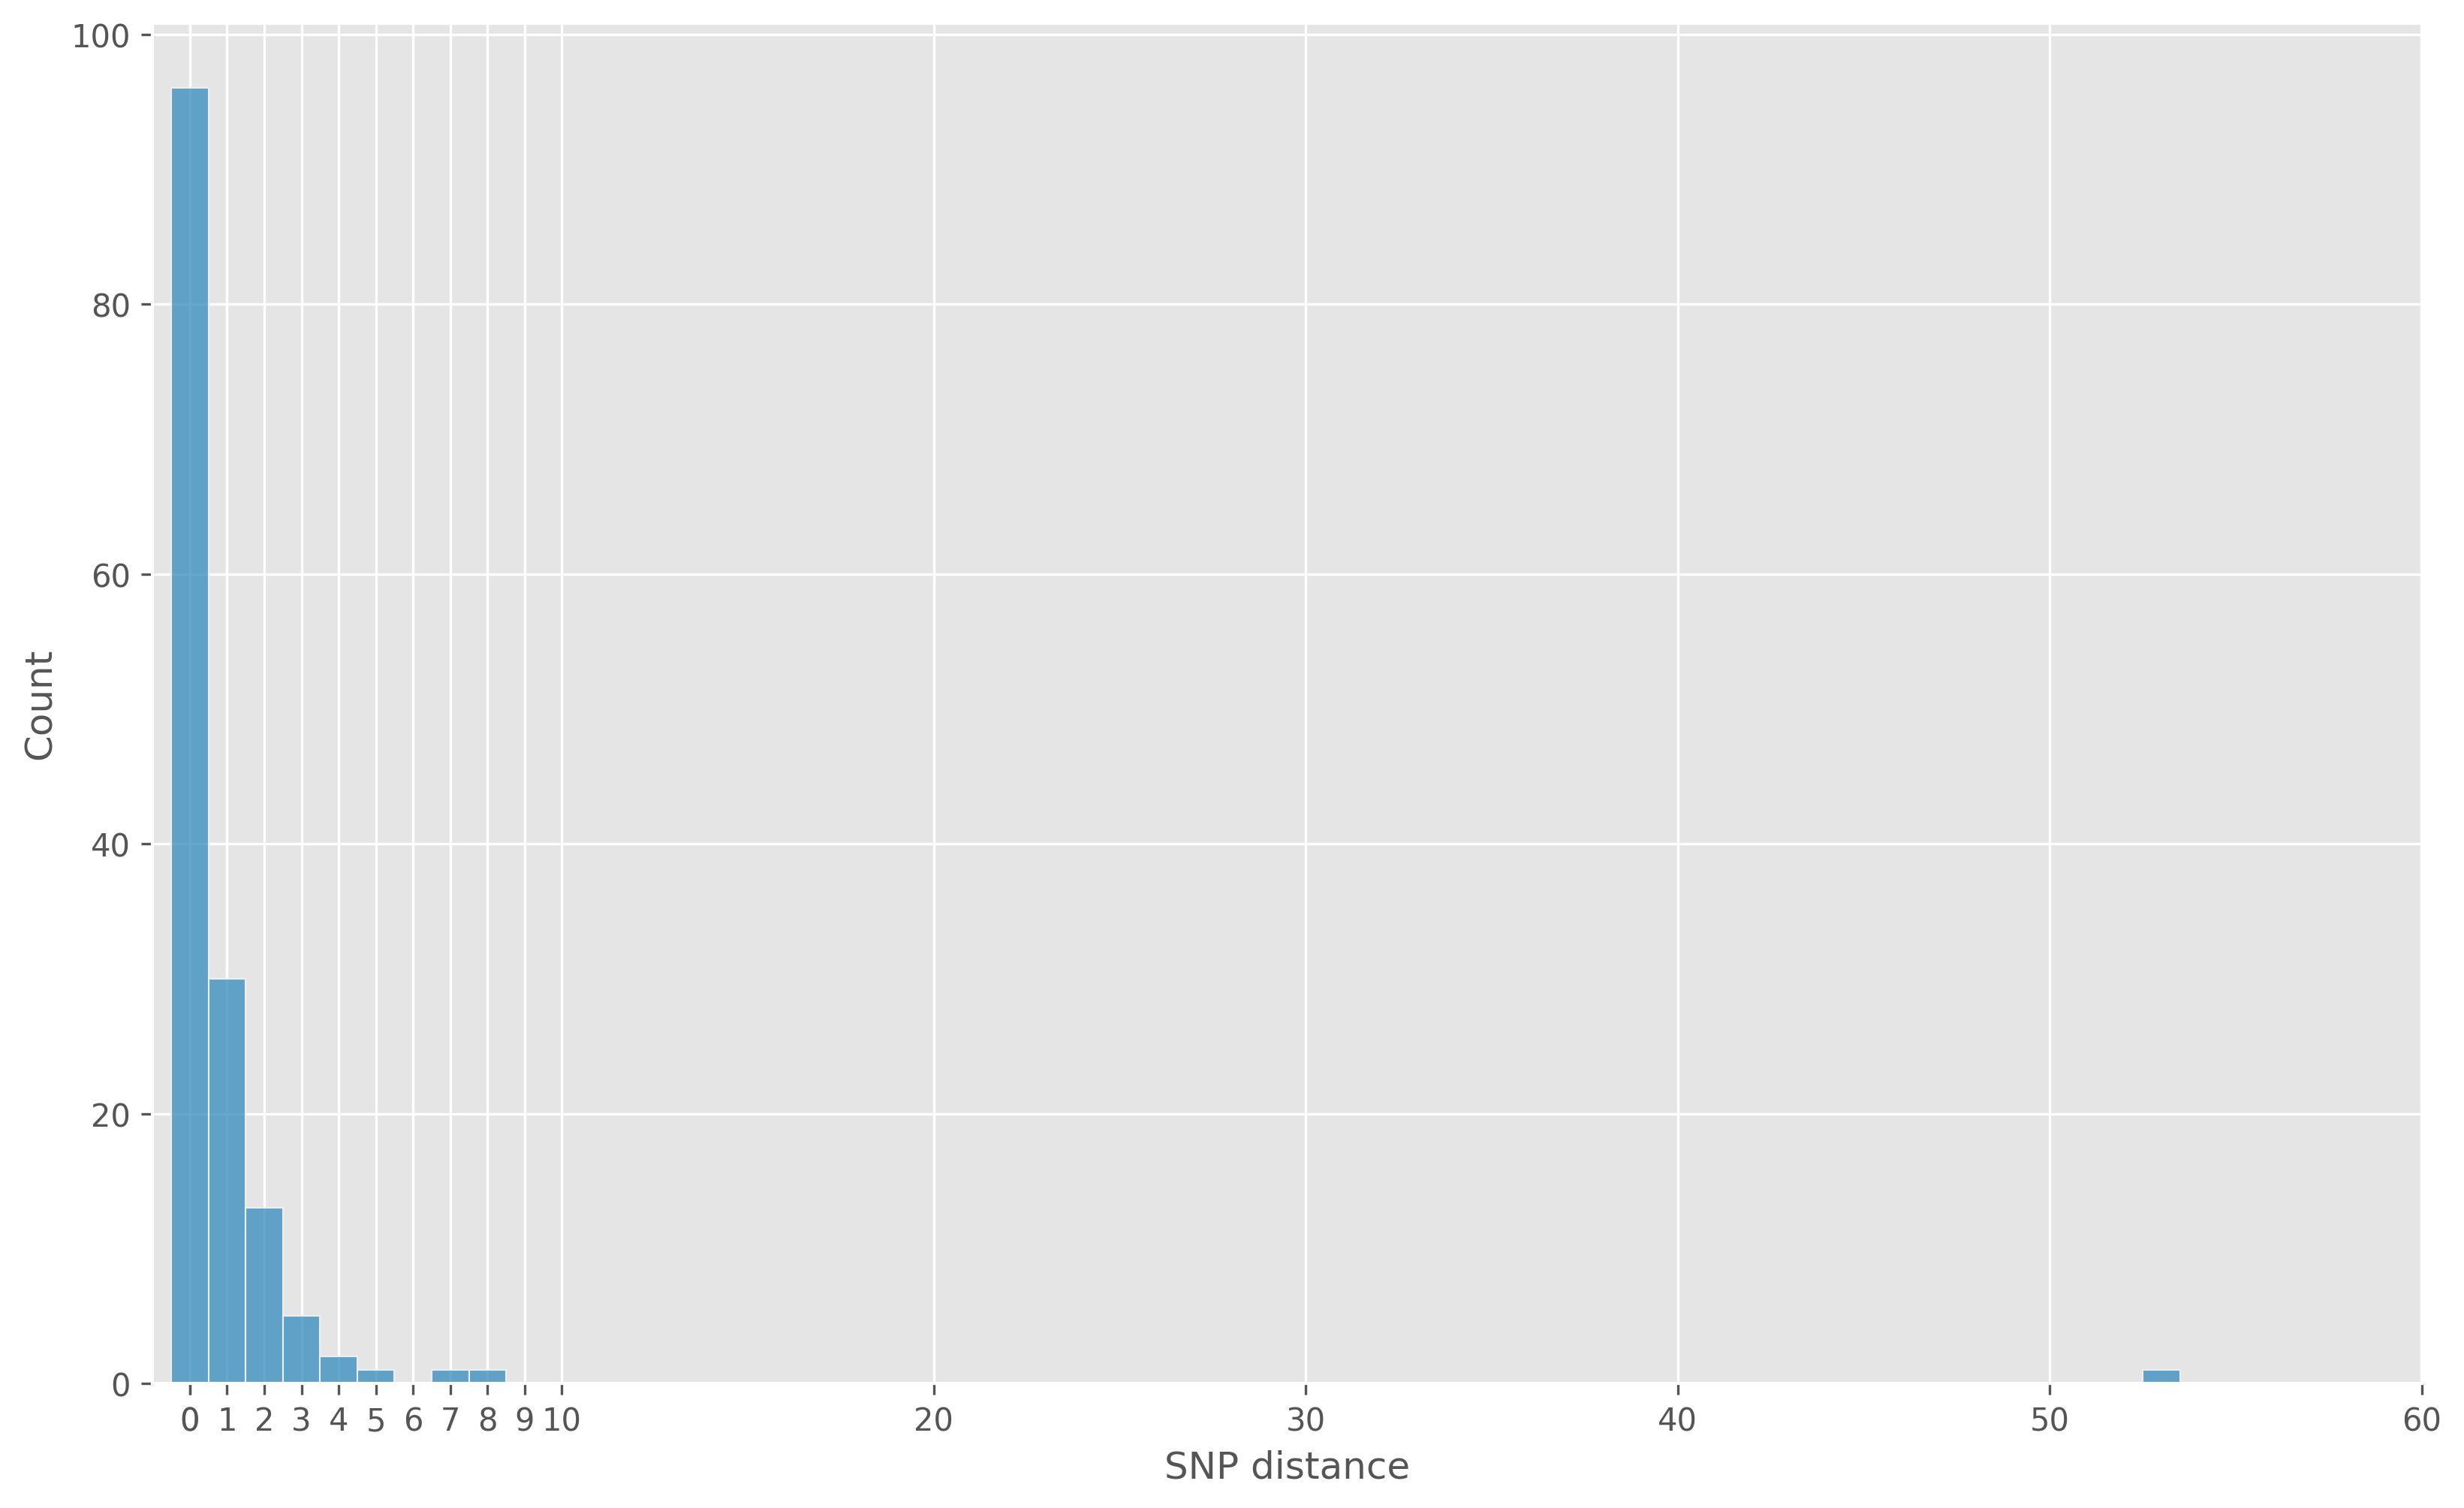
\includegraphics[width=0.90\columnwidth]{Chapter2/Figs/mixed_self_dist.png}
\caption{{Mixed modality "self-distance". This plot shows the SNP distance
(x-axis) between each sample's COMPASS (Illumina) and bcftools
(\ont{}) VCF calls.
{\label{fig:self-dist}}%
}}
\end{center}
\end{figure}

Next, we look at the pairwise SNP distance relationship, akin to that in \autoref{sec:snp-dist}. \autoref{fig:mixed-dotplot} shows the mixed SNP distances have a similar relationship to
the single-technology correlation in \autoref{fig:dotplot}. The difference here, however, is that
the y-axis represents the distance between one sample's Illumina data
and the other's Nanopore. There are twice as many data points in this plot though as the distance between two samples is not necessarily reciprocal for mixed modality distances (as we saw with the self-distances). That is, for two samples $a$ and $b$, $distance(a_I,b_N) \neq distance(a_N, b_I)$, where $I$ and $N$ refer to Illumina and \ont{} data respectively. In the zoomed inset window of \autoref{fig:mixed-dotplot}, there is a cluster of outlying points with a higher mixed distance than Illumina distance. All of these points relate to combinations of 6 samples in particular. These were investigated for evidence of a sample swap or poor quality data, but nothing was found to support such a claim. In reality, it just seems the \ont{} data for some of the samples is quite different to the Illumina data of the other samples.

\begin{figure}
\begin{center}
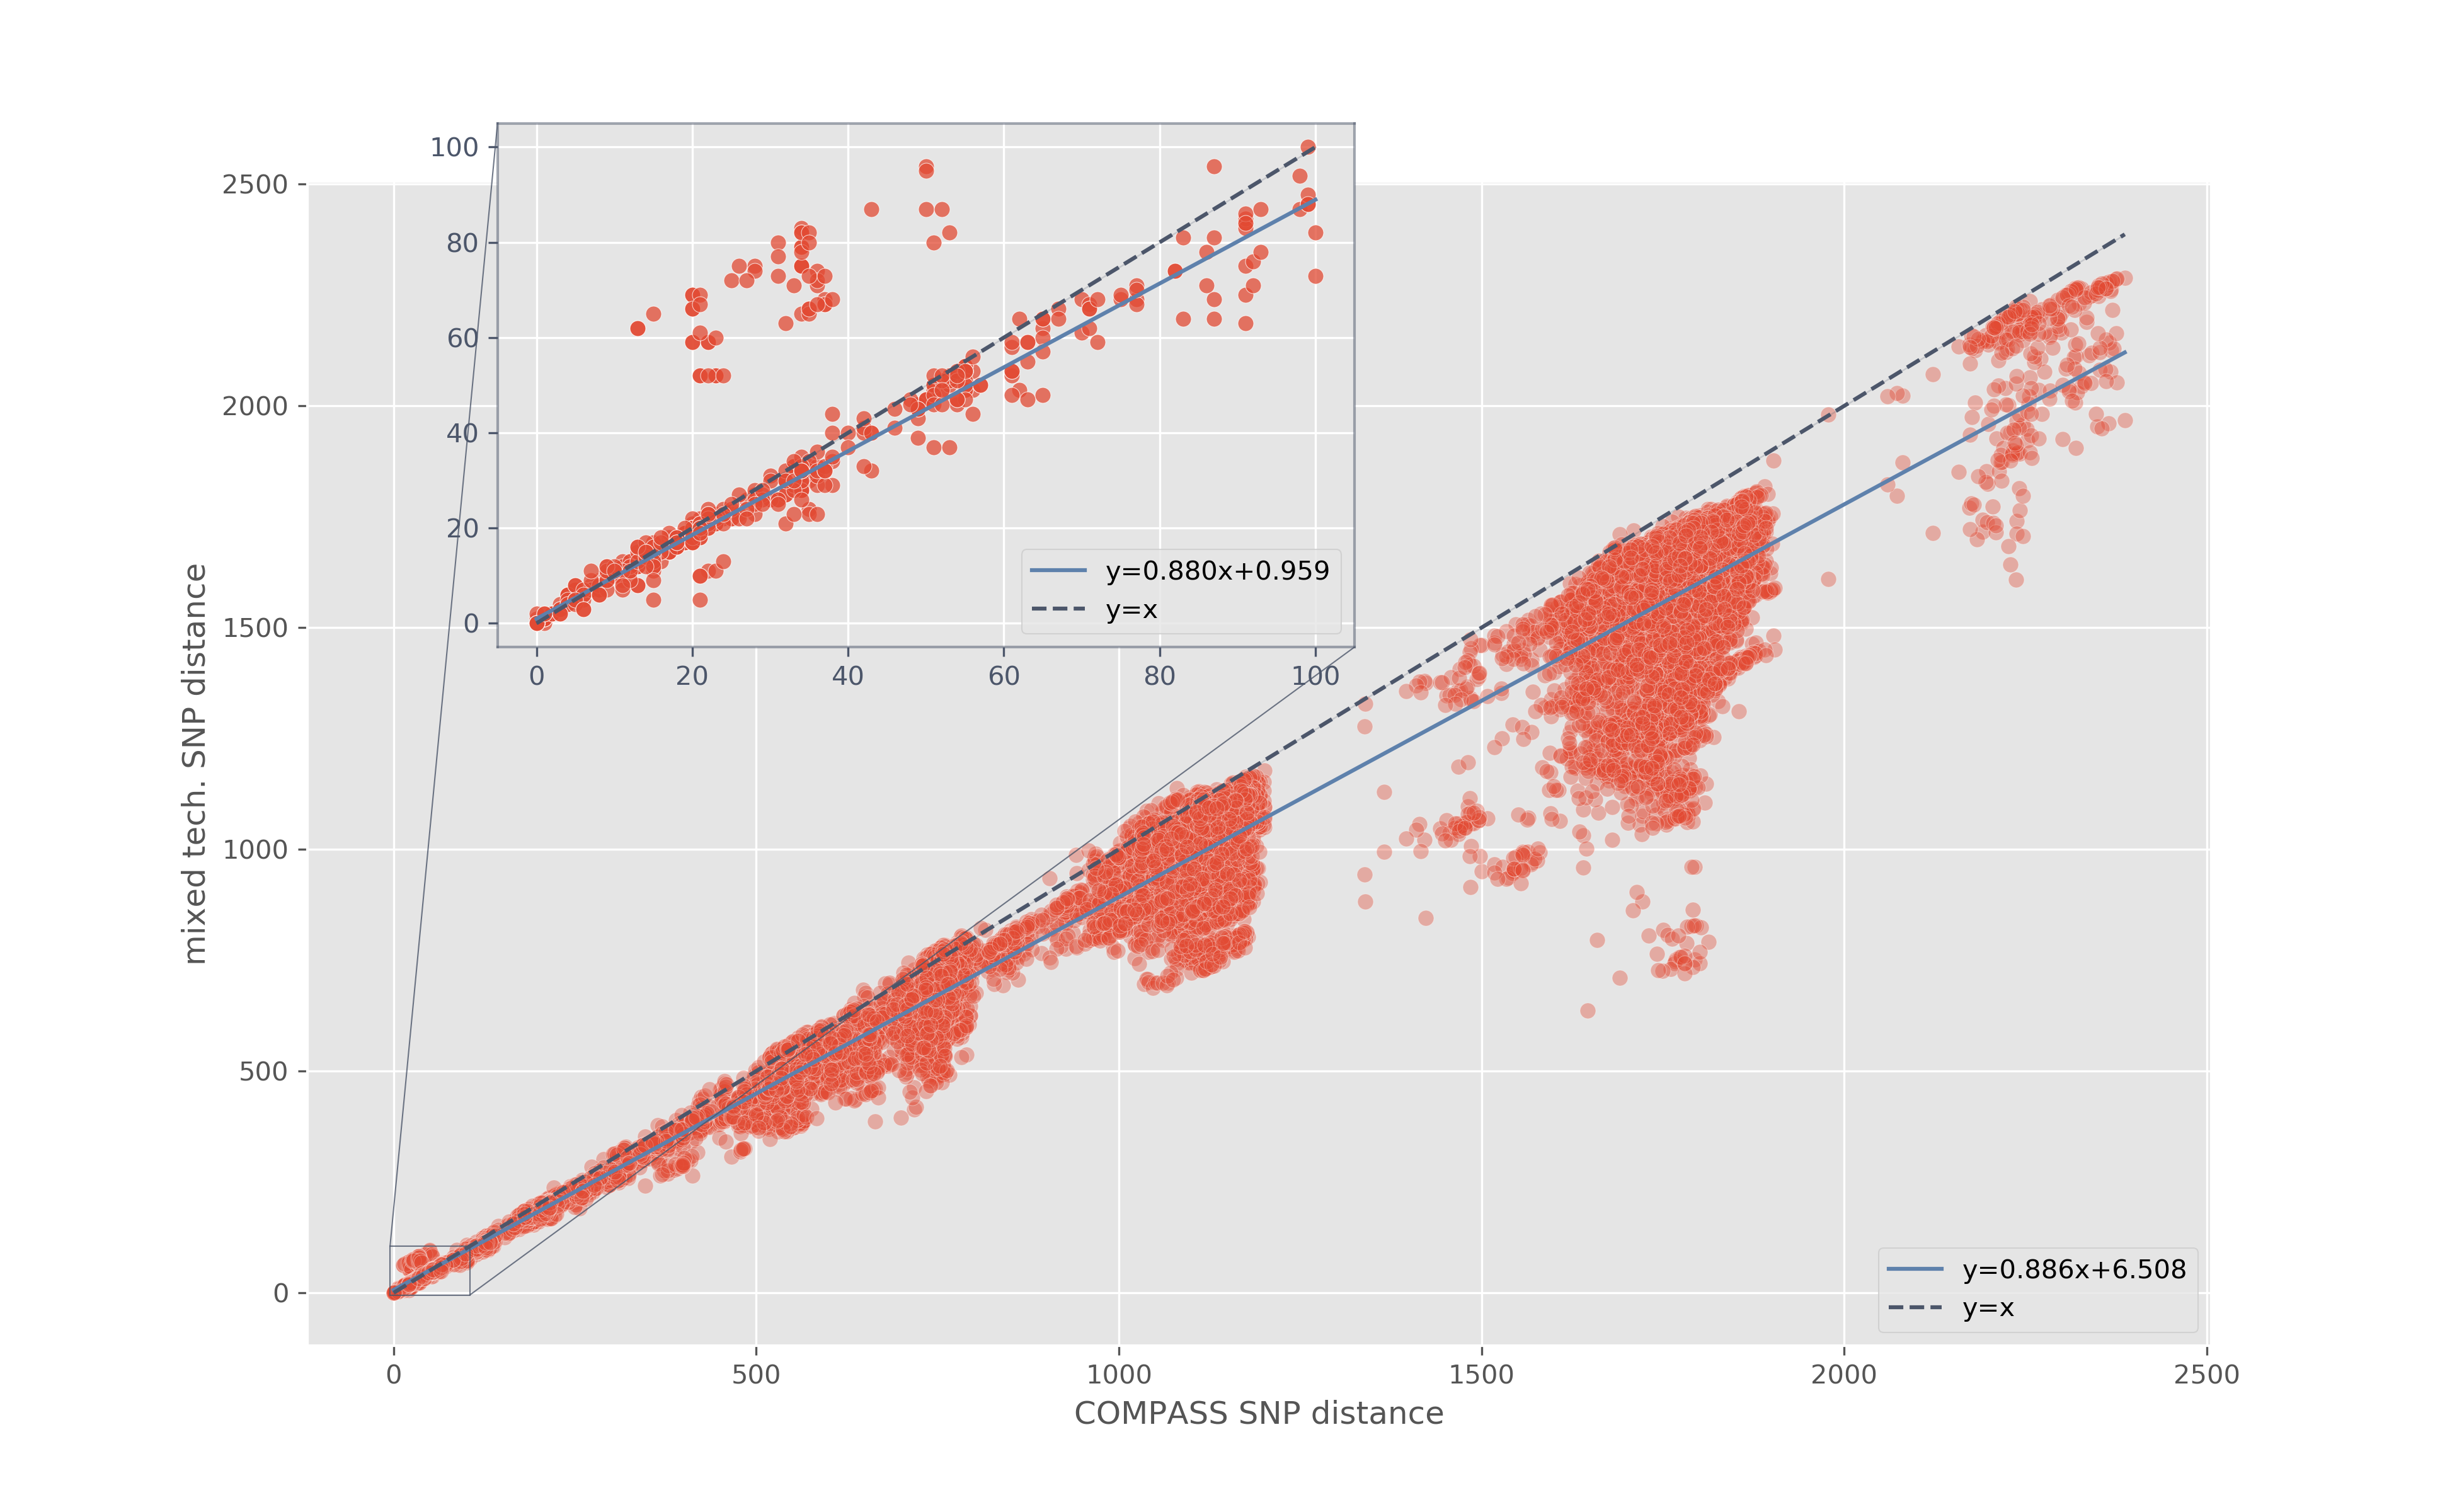
\includegraphics[width=0.90\columnwidth]{Chapter2/Figs/mixed-dotplot.png}
\caption{{The relationship of the distance between all pairs of samples based on
Illumina (COMPASS) VCF calls (X-axis) and mixed COMPASS-bcftools calls (Y-axis).
The black, dashed line indicates the relationship we would expect if the
distance between a pair of samples were the same for both approaches.
The blue line indicates the line of best fit based on fitting a robust
linear regression model to the data. The inset gives a closer look at
the relationship for all sample pairs where the COMPASS distance is less
than or equal to 100 SNPs. The legend indicates the linear equations for
the lines. Note: to prevent model skew, we do not include self-distance
pairs.
{\label{fig:mixed-dotplot}}%
}}
\end{center}
\end{figure}


We now examine transmission clusters for mixtures of Nanopore and
Illumina data using the same SNP thresholds used in \autoref{sec:clustering}. For the comparison of different
modalities we use the Illumina SNP thresholds. The mixture
ratios we investigate are 0.01, 0.05, 0.1, 0.25, 0.5, 0.75, and 0.9.
That is, for a ratio of 0.25, we \emph{randomly} allocate 25\% of the samples
to Nanopore and the remainder to Illumina. For each SNP threshold and
ratio, we calculate the XCR, SACR and SACP that the clustering produces
- using those ratio and threshold values. We repeat this process 1000
times for each threshold and ratio to simulate different mixtures of
sample-technology pairs. The simulation of so many different mixed pairs
is intended to provide insight into how robust clustering with mixtures
of sequencing datasets is likely to be. 
The results of these simulations
are shown in \autoref{fig:mixed-sims}. We found that for
all SNP thresholds and ratios, the median SACR was 1.0. In other words,
regardless of the Nanopore/Illumina mixture ratio, for all thresholds we
used, no sample is missed from its expected clustering. The SACP values
decrease somewhat as the ratio leans more towards Nanopore data.
However, the lowest median SACP value was 0.845, which is also the SACP
value obtained for the Nanopore-only clustering in
\autoref{sec:bcftools-clustering}. The XCR values tend to increase
slightly as more Nanopore samples are added. In the most extreme case,
0.057 was the highest XCR value in any simulation (SNP threshold 5).
Incidently, this is the same as the XCR obtained for the Nanopore-only
clustering of the same SNP threshold, which equates to 7 of the 122
non-clustered samples being clustered. However, regardless of the XCR,
no samples that should have been clustered were missed (on average).

\begin{figure}
\begin{center}
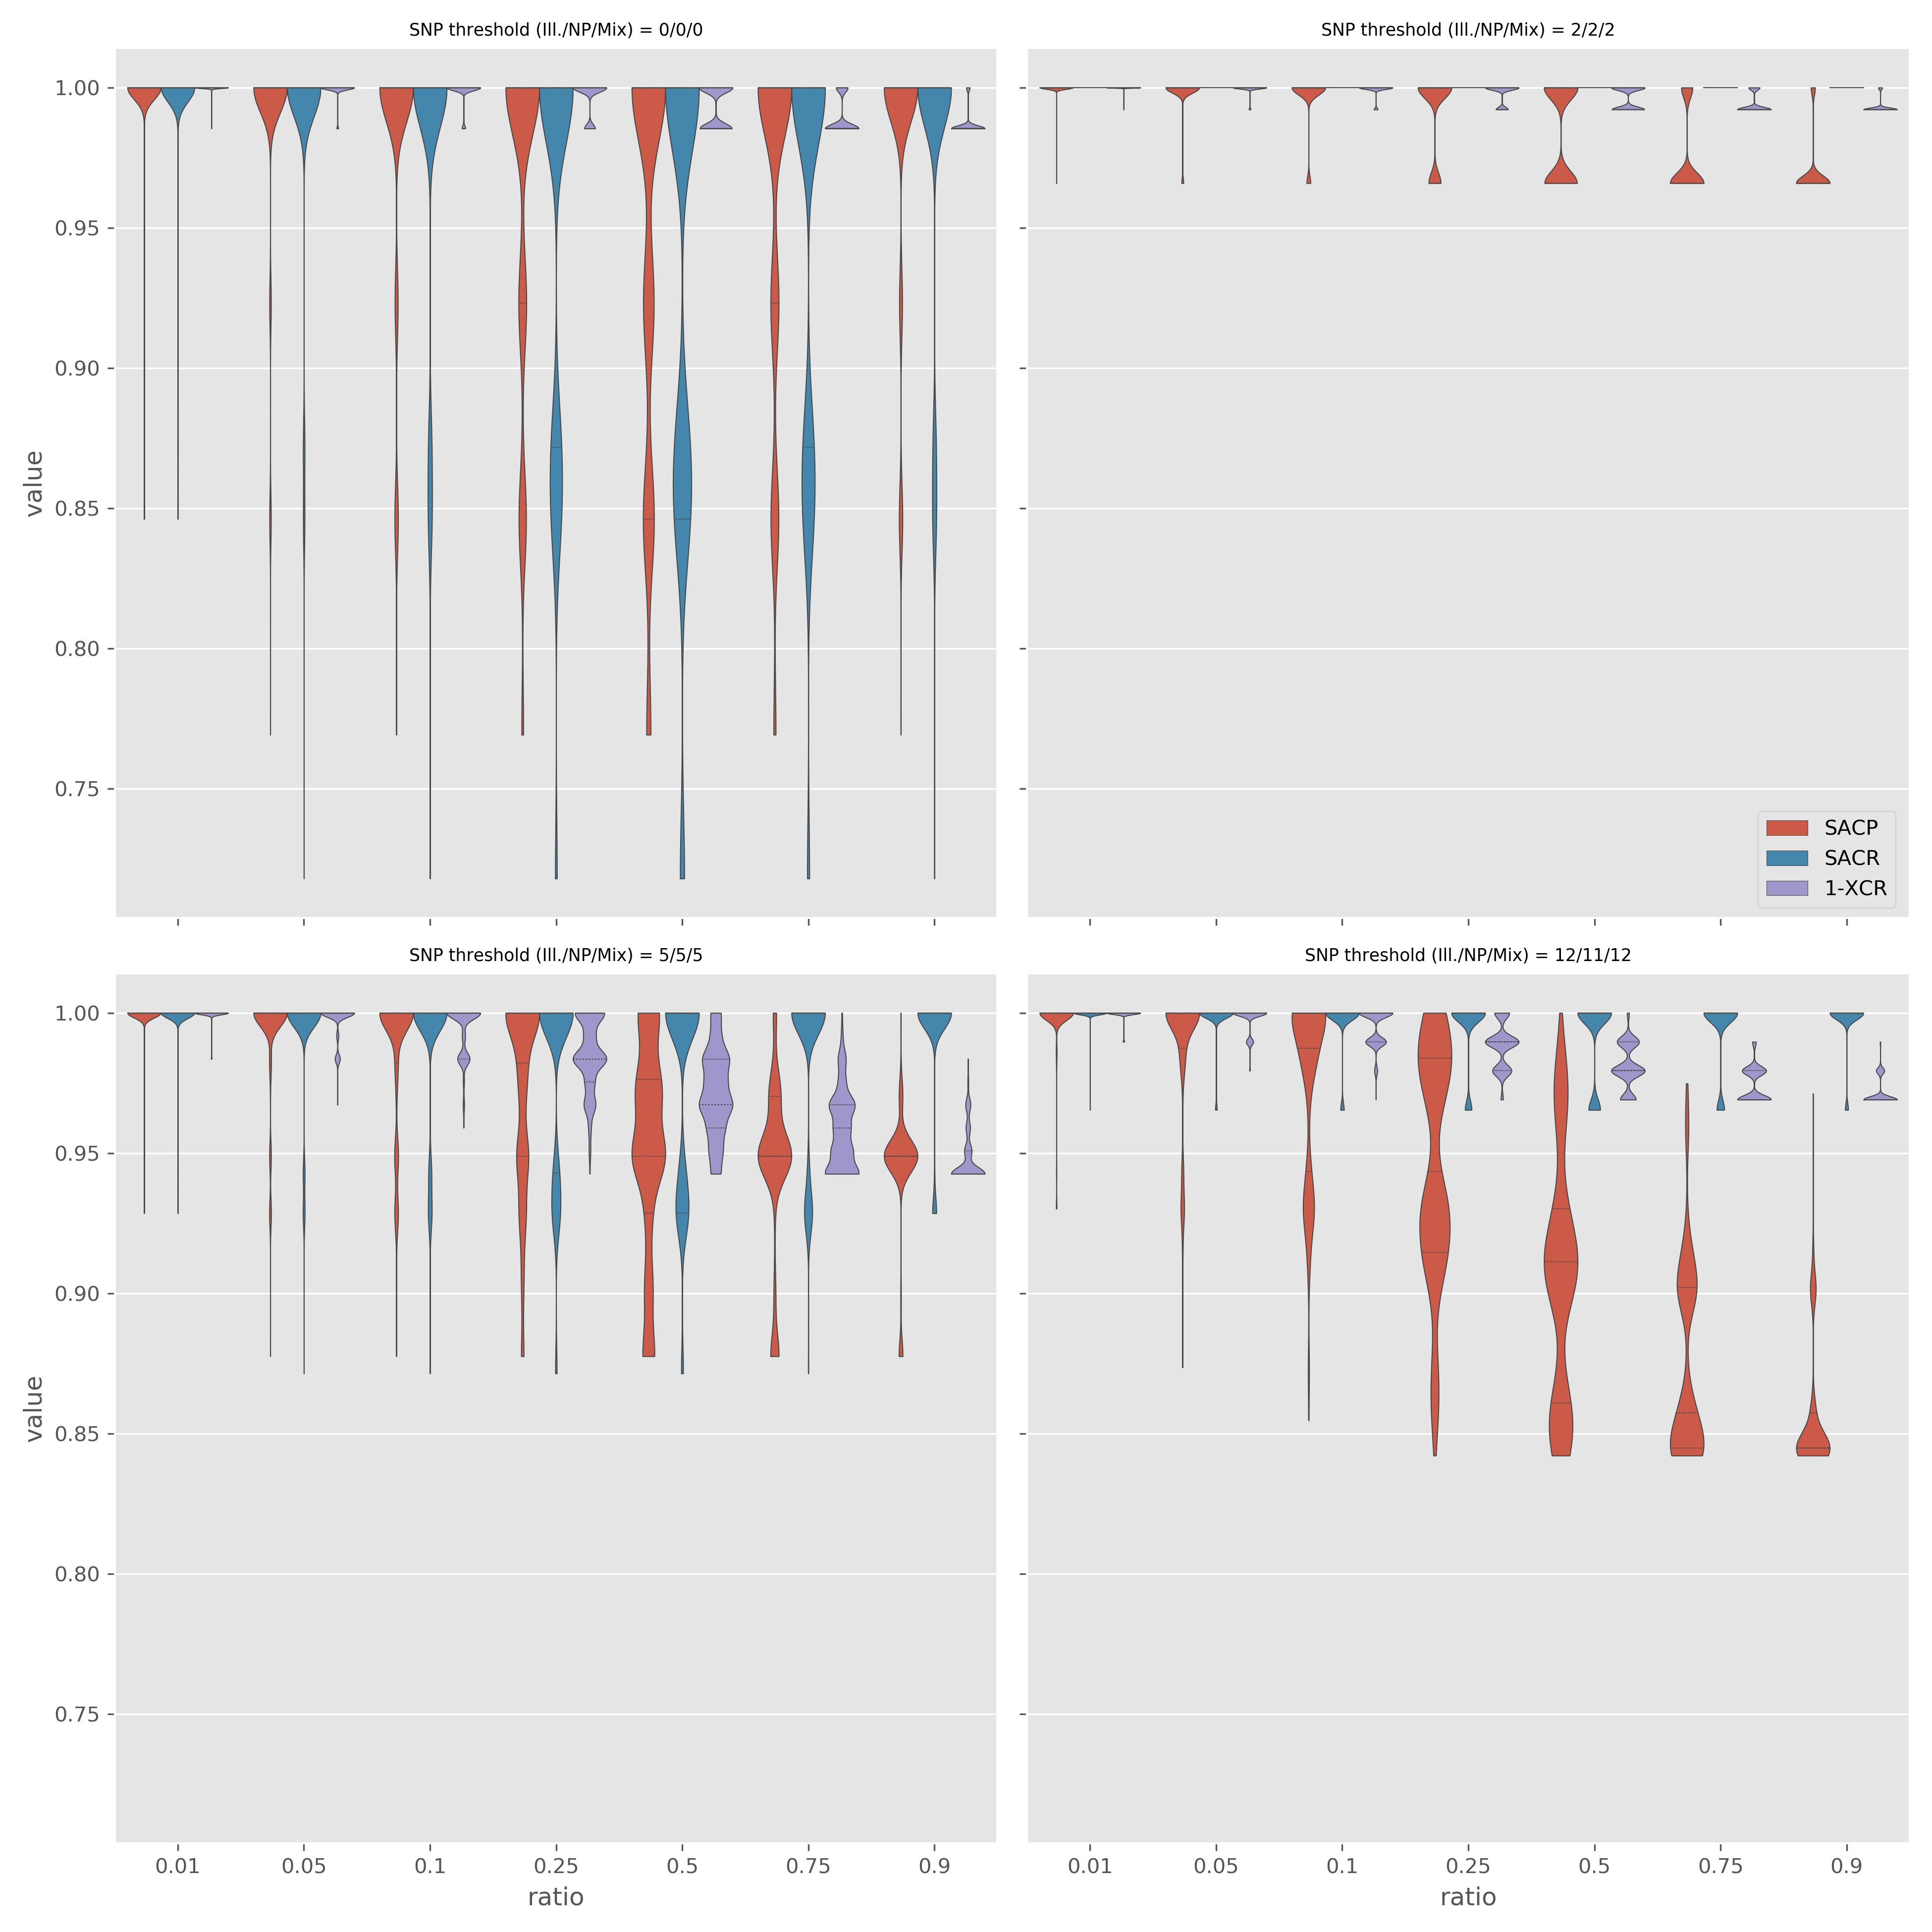
\includegraphics[width=0.90\columnwidth]{Chapter2/Figs/mixed_simulations.png}
\caption{{Simulating varying ratios (X-axis) of Nanopore/Illumina sample mixtures.
The different thresholds (subplots) indicate the cutoff for defining
samples as part of a cluster. The Y-axis depicts the Sample-Averaged
Cluster Precision and Recall (SACP/SACR) and Excess Clustering Rate
(XCR) distributions over all simulation runs (XCR is shown as (1-XCR)
for better axis-scaling). For each ratio/threshold combination we run
1000 simulations where the Nanopore and Illumina data is randomly split
into the relevant ratio and clusters are defined based on the relevant
threshold. The titles for each subplot indicate the SNP threshold used
when comparing Illumina (Ill.), Nanopore (NP), or mixed-technology
sample pairs.
{\label{fig:mixed-sims}}%
}}
\end{center}
\end{figure}

\subsection{Summary}

In this section we have shown that putative transmission clusters constructed using mixtures of Illumina and \ont{} data are consistent with those produced by Illumina data alone.

%=========================================================================

\section{Discussion}


Recent work from CITE \etal{} is the first effort to assess \ont{} for the clustering of samples based on genetic distance. While their work had a larger number of samples to ours (431), the SNP distance comparison details were very brief and were only presented for a subset of 14 samples. They present the results as a distance matrix and leave it as an exercise for the reader to compare the Illumina and \ont{} matrices. There is no quantification of the clustering similarities or investigation into whether Illumina and \ont{} data can be mixed for this application. In contrast, the work presented in this chapter provides a detailed analysis of all of these topics and much more.

In addition to the conventional single-reference variant-calling approach we also assessed the performance of the genome graph method developed in \autoref{chap:denovo} for \mtb{}. We built two \mtb{} population reference graphs with different variant densities. Intuition would say that the more variants in the \prg{}, the better the ability to find and call variants. However, we found the opposite. The sparse \prg{} produced marginally high precision and recall, on average, compared to its dense counterpart. As the computational resources required to construct and operate the sparse \prg{} are a lot less than the dense, we chose to use it for the subsequent analysis. The lack of improvement by adding more variants is inline with previosu work (CITE forge) that found a ceiling in the gains to adding more variants and that eventually it just causes complexity "blow ups" that manifest as increased computational resource requirements and reference ambiguity, all of which lead to a decay in overall performance. This is the same thing we see and note that many of the errors made by the dense \prg{} relate to shared \kmer{}s between alternate paths (generally in longer alleles) at sites in the graph, which in turn confuse the genotyping by adding coverage to multiple alleles. We investigate this complexity problem further in \autoref{chap:dst}.

The initial step in this chapter was the first investigation of the precision and recall of \ont{} variant calls for \mtb{}. Previous work (CITE lachlan/arnold) has only looked at one sample and only assessed variants in the \ppe{} genes. While there are a number of \ont{} variant callers that have recently been published, we chose to use bcftools due to its similarity to the Illumina strategy we are comparing to and also for its ease of use. Many of the \ont{} variant callers are neural network-based and require considerable bioinformatic knowledge to operate and in some circumstances require training of variant models. As our goal in this chapter is to investigate the use of \ont{} by public health laboratories and for clinical purposes we try to use methods that can be easily duplicated by others who may not have extensive bioinformatic training. It is difficult to directly compare our precision and the recall values to other \ont{} variant-calling work as we value precision higher than recall for the work in this chapter. Much of the \ont{} variant-calling benchmarks focus on balancing precision and recall. The precision from both \ont{} variant-calling strategies we analysed we consistent with Illumina and much higher than previous \ont{} benchmarks, however, we acknowledge the unfair comparison to other works given the different focus. Recall for both bcftools and \pandora{} were lower than Illumina - by quite a lot for \pandora{}. Compared to other \ont{} variant-calling work, the recall values we are able to obtain are a few percentage points below the best. Given we also report results for a variety of variant filtering stringencies, we hope these can be used by others who may place higher value on recall.
One unfortunate limitation of the variant-calling validation was the number of pacbio assemblies we could use. We sent 35 samples for pacbio sequencing, but due to technical difficulties in the sequencing lab, we only received sufficient data for assembly of 7 samples. These results would have been even more robust with 35 validation samples, however 7 is inline with the number used in other work (how does this number relate to other studies? gonorehea study? clair? shiga ecoli?)

% talk about the cluster similarity work being unique
We have outlined three new metrics for comparing the similarity of two transmission clustering approaches: the sample-averaged cluster recall (SACR) and precision (SACP), and the excess clustering rate (XCR). SACR and SACP are effectively just a "rebranding" of the set-similarity measure, the Tversky Index, with two parameters fixed. XCR has not been described elsewhere to the best of our knowledge. Cluster similarity is a rich field of research, however there are not many examples of this quantitative approach to comapring transmission cluster methods.
% https://www.sciencedirect.com/science/article/pii/S2352396418304249#s0025 (sec 2.3)
Use a clustering rate metric which is just the number of samples clustered, minus the number of clusters and then divided by the number of samples. 
% https://journals.plos.org/plosmedicine/article?id=10.1371/journal.pmed.1001387
Just focused on a large cluster but didnt really compare the clusterings
% beyond snp threshold use variation of information https://www.sciencedirect.com/science/article/pii/S0047259X06002016#!
Information theoretical framework that works well and not too disimilar to our approach. Variation of information which measures how much information is lost and gained in between two clustering approaches.
Our main reason to forego these previous methods in favour of our three has to do with the granularity of information. The studies mentioned all use a single metric to classify the performance of the clustering. However, using SACR, SACP and XCR, we know how changes in the methods for producing cluster impacts whethere samples are missed from clusters (SACR), wrongfully added to existing clusters (SACP), or if previously unclustered samples form their own new clusters (XCR). Such granularity allows users to tweak their clustering approach to meet their situtation. While we place higher value on SACR, others may find the reduction of cluster merging is of more importance and can focus on improving SACP instead. A single metric does not allow for this kind of targetted evaluation.

% citations or the below text
% 1, https://www.sciencedirect.com/science/article/pii/S0163445320300852
The first important finding of this chapter is that \ont{} data can produce transmission clusters comparable to Illumina. Indeed, bcftools and \pandora{} multi-sample do not miss any samples from clusters - the most important consideration for transmission chain investigation (find a source). This result agrees with the only other \mtb{} study of this kind (CITE NY). Additionally, \ont{}'s suitability for transmission investigation has also been confirmed for other pathogens such as Human metapneumovirus (CITE 1), Shiga toxin-producing \ecoli{}, and  Neisseria gonorrhoeae.

It is important to highlight that the focus of this work is not intended as a variant-calling benchmark for WGS technologies. We acknowledge that COMPASS may not be the best Illumina-based varinat calling strategy. Indeed, there are many bioinformatic pipelines available for the analysis of \mtb{} Illumina data, all with different results from one another (CITE tb pipeline benchmark paper). Instead, we take an approach being used "in the wild" - by PHE - and ask whether \ont{} can provide information of the same quality? For the application of clustering genomes based on genetic distance, we find \ont{} does provide comparable information when using bcftools to call variants. In addition, we found that using the multi-sample comparison mode of \pandora{} we also succeed in cluster all samples that should be clustered, albeit at the cost of adding more false positive connections. While the precision of variant calls for \pandora{} was as high as Illumina, the clustering produced by the single-sample mode was much worse than the other approaches. In general, the distances between samples based on \pandora{}'s single sample variant calls were much higher than the Illumina data suggested they should be. One point that contributes to this difference is the subtle difference in how we generate the \pandora{} single-sample consensus sequence. The main difference compared to bcftools and Illumina is when a position in the H37Rv reference genome is missing from the \pandora{} single-sample VCF, we assume it is the reference position, rather than nullifying it. We initially took the nullify approach for missing positions, but found this lead to a huge under-calling of the distances. The bulk of the extra pairwise differences (false positives) called by \pandora{} single-sample were positions missing from one of the samples and present in the other. In 96\% of those false positive the position was filtered out in the COMPASS and bcftools VCFs due to evidence of heterozygosity. Ultimately, this issue stems from the fact that COMPASS and bcftools make calls at all positions of the genome with read depth, while \pandora{} only makes calls at sites with alternate alleles. A new approach for calculating the distance between \pandora{} single-sample VCFs cerainly warrants further investigation.
The difference in clustering obtained by the two \pandora{} approaches highlights their intended use cases. The multi-sample approach, `compare`, was designed for allowing the comparison of collections of samples. It integrates information from \emph{all} samples by selecting a consensus sequence that best approximates them, and then calling variation against that consensus. This approach allows for easily identifying differences between samples as the VCF produced by `compare` has genotype information for all samples at all sites. While the `compare` protocol did not miss any samples from their correct clusters, it did incorrectly join some clusters and create new clusters from samples Illumina deemed singletons. This incorrect joining of samples and clusters is not entirely unexpected. Incorrectly joining samples indicates that the distances between samples is lower than expected for `compare` (this is supported by \autoref{fig:dotplot}). Given the \pandora{} variant calls showed significantly lower recall than COMPASS and bcftools (see \autoref{fig:prec-recall-filters}), a smaller distance between samples is expected. One obviuous way of trying to improve recall is by masking less of the genome (see \autoref{app:mask}). 

In addition to acknowledging that this variant-calling approach may not be the absolute best approach, we also acknowledge that SNP distance clustering also has shortcomings. Again, our intention is not to claim to be the best clustering method, but to mimic the process currently used by PHE - which is the SNP threshold approach used here. Stimson \etal{} recently published an important study shwoing that mixing SNP threshold and epidemiological data can lead to superior transmission chain reconstruction comapred to SNP threshold alone. With the establishement of \ont{}'s ability to provide accurate SNP threshold-based clusters it seems certain that the inclusion of epidemiological data using the same approach as Stimson \etal{} can only improve inference for this application.

% mixed data
%  gonnorhea paper has median self distance of 5
% 1. https://www.nature.com/articles/s41598-020-74656-y#Sec2
% 2. https://link.springer.com/article/10.1186/s12864-021-07460-1
With the knowledge that \ont{} can also be used for inferring chains of transmission for \mtb{} we ask a logical next question: can transmission clusters be accurately constructed from a mixture of \ont{} and Illumina data? As \ont{} sequencing becomes more ubiquitous it seems inevitable that groups using different sequencing modalities will want to compare data. We find that they absolutely can be mixed and produce clusters consistent with Illumina-only data. This is the first known case (to the author's knowledge) of testing this mixing of data for \mtb{}. The mixture of \ont{} and Illumina consensus sequences has been done for hepatitis C (2); also finding the modalities can be mixed without a degradation of results. Others have also compared phylogenetic trees constructed from a combination of the two modalities (1 - get another), but ours is the first SNP threshold-based clustering to use mixtures of technologies that we know of. 
At a range of different mixture ratios we randomly assign samples to different sequencing technologies and assess the clustering. We repeat this random division of samples 1000 times in order give an idea of the potential spread of results. 

In conclusion, the work in this chapter has shown that \ont{} data can produce transmission clusters consistent with those from Illumina. Additionally, it is also possible to mix data of the two modalities and still produce concordant clusters. We have also provided the first evaluation of \ont{} variant-calling for \mtb{}, and three new metrics for assessing transmission cluster similarity.
These results are consistent with another \mtb{} \ont{}-based transmission cluster study and similar work on other bacterial and viral pathogens. As a result, we believe \ont{} sequencing has reached sufficient quality to be considered for public health use for transmission clustering.

%=========================================================================

\section{Future work}

\subsection{Dataset with known epidemiological information}
Perhaps the most important follow up of the work in this chapter is to gather a dataset with epidemiologically linked cases and known transmission clusters. While these datasets do exist for Illumina data, there are none yet with matched Illumina and \ont{} sequencing. Matched sequencing data is necessary to know that differences in DNA are solely driven by sequencing technology. A dataset with strong evidence for transmission clusters would remove the main limitation to this chapter and be an even stronger statement for the use of \ont{} sequencing in public health laboratories.

\subsection{Computational performance of variant calling}
% bcftools baq work https://github.com/mbhall88/head_to_head_pipeline/issues/38#issuecomment-661680608
In \autoref{sec:var-call-comp-perf} we assessed the time and memory usage for variant calling for bcftools and \pandora{}. bcftools in particular had, in the worst case, the highest memory and CPU of the callers. Nearly all of this time and memory is spent realigning reads in the pileup in order to calculate the base alignment quality (BAQ) score. When we disabled this BAQ setting for one sample, the CPU time dropped from 3 hours to 30 minutes (6-fold decrease) and peak memory reduced from 58GB to 70MB (829-fold decrease). However, this did come at the cost of a slight reduction in precision and recall. As we write this chapter though, the newest release of bcftools (version 1.13) has addressed this problem by only doing the BAQ realignment in areas overlapping problematic indel sites. Their testing shows this drastically reduces the peak memory and the overall runtime and actually \emph{increased} recall (the realignment can sometimes be detrimental). As such, an obvious task for future development would be to rerun this analysis with the latest bcftools version and assess the expected changes in computational resource usage and recall.
Much of the memory and CPU time used in the \pandora{} pipelines lies in updating the multiple sequence alignments used to build the \prg{} after novel variants have been added. Recent work by Leandro Ishi in our research group has produced a prototype of the \makeprg{} program that significantly reduces the time and memory required to update the \prg{} (as discussed in \autoref{sec:denovo-fw}). It remains to be seen whether these update will also improve \pandora{}'s precision and/or recall, but it will certainly improve the computational requirements. 

\subsection{Improving \prg{} construction}
%  construction of prg maybe better by extracting consensus sequence for each sample rather than applying variants individually - refer to chap3
The current process for building the \mtb{} \prg{} is, for each locus, to apply a single VCF alternate allele to the reference sequence for that locus and collect all of these mutated sequence into a multi-sequence FASTA file. One limitation of this approach is that variants do not always occur in isolation like this. Where this becomes important is when turning an MSA into a \prg{} with \makeprg{}. An important parameter in this process is the minimum match length, $m$. When two variants are within $m$ positions of each other, creating two separate sequences for them (as we do) creates alternate paths in the \prg{}, with neither path containing the correct allele combination. This is best understood with an example. Say we set $m$ to 3 and have two variants at position 2 and 4. The first variant is a SNP changing an A to a T and the second a C to a G. The two mutated sequences we produce for these two variants is ATAC and the other is AAAG. Because these two sequences do not have a minimum match length of 3 or more, they become two alternate paths in the \prg{}. However, these two variants come from the same sample, so in reality the true sequence is ATAG. When using the \prg{} containing the two alternate alleles, if we have a sample that contains both of the variants (i.e. ATAG) it does not match either of the two alleles, even though they come from a sample with ATAG at this site. Ultimately, we rely on the \denovo{} variant discovery from \autoref{chap:denovo} to fix this. Unfortunately it doesn't always do this and as we will see in \autoref{chap:dst}, even if we \denovo{} discovery adds the correct allele, ATAG, we have three alleles now that could share minimizing \kmer{}s and this lead to read coverage on all three. One solution to this would be the construct the \prg{} by applying \emph{all} the variants from a sample at a given locus in one sequence - rather than a sequence for each variant. The reason we did not construct the \prg{} in this fashion in \autoref{sec:tbprg} was that for each locus, we would have had $n$ sequences - where $n$ is the number of samples - to perform an MSA on. We chose to apply single variants as the number of variants in a locus was, in most cases, much smaller than $n$ and thus the MSA ran much quicker and used much less memory.
% improving masking of prg could help recall
In addition to improvements in the way variants are added, there are improvements that can be made in the masking of loci. Our current method of removing loci from the \prg{} when they have 30\% or more overlap with a genome mask (\autoref{app:mask}) leads to approximately 6\% of loci being removed, or 10\% of the genome. As the genome mask used covers 7.4\% of the genome, we remove more than is necessary and this impacts our recall. A recent study by Marin \etal{} has shown this genome mask to be excessive and present a new mask that covers only 4\% of the H37Rv reference genome \cite{marin2021}. So a first step for improving the recall of \pandora{} would be to rebuild the \prg{} using this new mask.